%**************************************%
%* Generated from MathBook XML source *%
%*    on 2016-07-21T16:56:38-04:00    *%
%*                                    *%
%*   http://mathbook.pugetsound.edu   *%
%*                                    *%
%**************************************%
\documentclass[10pt,]{book}
%% Load geometry package to allow page margin adjustments
\usepackage{geometry}
\geometry{letterpaper,total={5.0in,9.0in}}
%% Custom Preamble Entries, early (use latex.preamble.early)
%% Inline math delimiters, \(, \), need to be robust
%% 2016-01-31:  latexrelease.sty  supersedes  fixltx2e.sty
%% If  latexrelease.sty  exists, bugfix is in kernel
%% If not, bugfix is in  fixltx2e.sty
%% See:  https://tug.org/TUGboat/tb36-3/tb114ltnews22.pdf
%% and read "Fewer fragile commands" in distribution's  latexchanges.pdf
\IfFileExists{latexrelease.sty}{}{\usepackage{fixltx2e}}
%% Page Layout Adjustments (latex.geometry)
%% This LaTeX file may be compiled with pdflatex or xelatex
%% The following provides engine-specific capabilities
%% Generally, xelatex will do better languages other than US English
%% You can pick from the conditional if you will only ever use one engine
\usepackage{ifthen}
\usepackage{ifxetex}
\ifthenelse{\boolean{xetex}}{%
%% begin: xelatex-specific configuration
%% fontspec package will make Latin Modern (lmodern) the default font
\usepackage{xltxtra}
\usepackage{fontspec}
%% end: xelatex-specific configuration
}{%
%% begin: pdflatex-specific configuration
%% translate common Unicode to their LaTeX equivalents
%% Also, fontenc with T1 makes CM-Super the default font
%% (\input{ix-utf8enc.dfu} from the "inputenx" package is possible addition (broken?)
\usepackage[T1]{fontenc}
\usepackage[utf8]{inputenc}
%% end: pdflatex-specific configuration
}
%% Monospace font: Inconsolata (zi4)
%% Sponsored by TUG: http://levien.com/type/myfonts/inconsolata.html
%% See package documentation for excellent instructions
%% One caveat, seem to need full file name to locate OTF files
%% Loads the "upquote" package as needed, so we don't have to
%% Upright quotes might come from the  textcomp  package, which we also use
%% We employ the shapely \ell to match Google Font version
%% pdflatex: "varqu" option produces best upright quotes
%% xelatex: add StylisticSet 1 for shapely \ell
%% xelatex: add StylisticSet 2 for plain zero
%% xelatex: we add StylisticSet 3 for upright quotes
%% 
\ifthenelse{\boolean{xetex}}{%
%% begin: xelatex-specific monospace font
\usepackage{zi4}
\setmonofont[BoldFont=Inconsolatazi4-Bold.otf,StylisticSet={1,3}]{Inconsolatazi4-Regular.otf}
%% end: xelatex-specific monospace font
}{%
%% begin: pdflatex-specific monospace font
\usepackage[varqu]{zi4}
%% end: pdflatex-specific monospace font
}
%% Symbols, align environment, bracket-matrix
\usepackage{amsmath}
\usepackage{amssymb}
%% allow more columns to a matrix
%% can make this even bigger by overriding with  latex.preamble.late  processing option
\setcounter{MaxMatrixCols}{30}
%% Semantic Macros
%% To preserve meaning in a LaTeX file
%% Only defined here if required in this document
%% Used for inline definitions of terms
\newcommand{\terminology}[1]{\textbf{#1}}
%% Used for fillin answer blank
%% Argument is length in em
\newcommand{\fillin}[1]{\rule{#1em}{0.1ex}}
%% Subdivision Numbering, Chapters, Sections, Subsections, etc
%% Subdivision numbers may be turned off at some level ("depth")
%% A section *always* has depth 1, contrary to us counting from the document root
%% The latex default is 3.  If a larger number is present here, then
%% removing this command may make some cross-references ambiguous
%% The precursor variable $numbering-maxlevel is checked for consistency in the common XSL file
\setcounter{secnumdepth}{3}
%% Environments with amsthm package
%% Theorem-like environments in "plain" style, with or without proof
\usepackage{amsthm}
\theoremstyle{plain}
%% Numbering for Theorems, Conjectures, Examples, Figures, etc
%% Controlled by  numbering.theorems.level  processing parameter
%% Always need a theorem environment to set base numbering scheme
%% even if document has no theorems (but has other environments)
\newtheorem{theorem}{Key Idea}[chapter]
%% Only variants actually used in document appear here
%% Style is like a theorem, and for statements without proofs
%% Numbering: all theorem-like numbered consecutively
%% i.e. Corollary 4.3 follows Theorem 4.2
%% Remark-like environments, normal text
%% Numbering is in sync with theorems, etc
\theoremstyle{definition}
\newtheorem{remark}[theorem]{Remark}
%% Example-like environments, normal text
%% Numbering is in sync with theorems, etc
\theoremstyle{definition}
\newtheorem{example}[theorem]{Example}
%% Numbering for Projects (independent of others)
%% Controlled by  numbering.projects.level  processing parameter
%% Always need a project environment to set base numbering scheme
%% even if document has no projectss (but has other blocks)
\newtheorem{project}{Project}[chapter]
%% Project-like environments, normal text
\theoremstyle{definition}
\newtheorem{investigation}[project]{Investigation}
%% assemblage: minimally structured content, high visibility presentation
%% Package for breakable highlight boxes
\usepackage{mdframed}
%% assemblage style
\mdfdefinestyle{assemblage}{framemethod=default,linewidth=2pt,roundcorner=16pt,backgroundcolor=black!05}
%% Miscellaneous environments, normal text
%% Numbering for inline exercises and lists is in sync with theorems, etc
\theoremstyle{definition}
\newtheorem{exercise}[theorem]{Exercise}
%% Localize LaTeX supplied names (possibly none)
\renewcommand*{\appendixname}{Appendix}
\renewcommand*{\chaptername}{Chapter}
%% Equation Numbering
%% Controlled by  numbering.equations.level  processing parameter
\numberwithin{equation}{section}
%% For improved tables
\usepackage{array}
%% Some extra height on each row is desirable, especially with horizontal rules
%% Increment determined experimentally
\setlength{\extrarowheight}{0.2ex}
%% Define variable thickness horizontal rules, full and partial
%% Thicknesses are 0.03, 0.05, 0.08 in the  booktabs  package
\makeatletter
\newcommand{\hrulethin}  {\noalign{\hrule height 0.04em}}
\newcommand{\hrulemedium}{\noalign{\hrule height 0.07em}}
\newcommand{\hrulethick} {\noalign{\hrule height 0.11em}}
%% We preserve a copy of the \setlength package before other
%% packages (extpfeil) get a chance to load packages that redefine it
\let\oldsetlength\setlength
\newlength{\Oldarrayrulewidth}
\newcommand{\crulethin}[1]%
{\noalign{\global\oldsetlength{\Oldarrayrulewidth}{\arrayrulewidth}}%
\noalign{\global\oldsetlength{\arrayrulewidth}{0.04em}}\cline{#1}%
\noalign{\global\oldsetlength{\arrayrulewidth}{\Oldarrayrulewidth}}}%
\newcommand{\crulemedium}[1]%
{\noalign{\global\oldsetlength{\Oldarrayrulewidth}{\arrayrulewidth}}%
\noalign{\global\oldsetlength{\arrayrulewidth}{0.07em}}\cline{#1}%
\noalign{\global\oldsetlength{\arrayrulewidth}{\Oldarrayrulewidth}}}
\newcommand{\crulethick}[1]%
{\noalign{\global\oldsetlength{\Oldarrayrulewidth}{\arrayrulewidth}}%
\noalign{\global\oldsetlength{\arrayrulewidth}{0.11em}}\cline{#1}%
\noalign{\global\oldsetlength{\arrayrulewidth}{\Oldarrayrulewidth}}}
%% Single letter column specifiers defined via array package
\newcolumntype{A}{!{\vrule width 0.04em}}
\newcolumntype{B}{!{\vrule width 0.07em}}
\newcolumntype{C}{!{\vrule width 0.11em}}
\makeatother
%% Figures, Tables, Listings, Floats
%% The [H]ere option of the float package fixes floats in-place,
%% in deference to web usage, where floats are totally irrelevant
%% We re/define the figure, table and listing environments, if used
%%   1) New mbxfigure and/or mbxtable environments are defined with float package
%%   2) Standard LaTeX environments redefined to use new environments
%%   3) Standard LaTeX environments redefined to step theorem counter
%%   4) Counter for new environments is set to the theorem counter before caption
%% You can remove all this figure/table setup, to restore standard LaTeX behavior
%% HOWEVER, numbering of figures/tables AND theorems/examples/remarks, etc
%% WILL ALL de-synchronize with the numbering in the HTML version
%% You can remove the [H] argument of the \newfloat command, to allow flotation and 
%% preserve numbering, BUT the numbering may then appear "out-of-order"
\usepackage{float}
\usepackage[bf]{caption} % http://tex.stackexchange.com/questions/95631/defining-a-new-type-of-floating-environment 
\usepackage{newfloat}
% Side-by-side elements need careful treatement for aligning captions, see: 
% http://tex.stackexchange.com/questions/230335/vertically-aligning-minipages-subfigures-and-subtables-not-with-baseline 
\usepackage{stackengine,ifthen}
\newcounter{figstack}
\newcounter{figindex}
\newlength\fight
\newcommand\pushValignCaptionBottom[5][b]{%
\stepcounter{figstack}%
\expandafter\def\csname %
figalign\romannumeral\value{figstack}\endcsname{#1}%
\expandafter\def\csname %
figtype\romannumeral\value{figstack}\endcsname{#2}%
\expandafter\def\csname %
figwd\romannumeral\value{figstack}\endcsname{#3}%
\expandafter\def\csname %
figcontent\romannumeral\value{figstack}\endcsname{#4}%
\expandafter\def\csname %
figcap\romannumeral\value{figstack}\endcsname{#5}%
\setbox0=\hbox{%
\begin{#2}{#3}#4\end{#2}}%
\ifdim\dimexpr\ht0+\dp0\relax>\fight\global\setlength{\fight}{%
\dimexpr\ht0+\dp0\relax}\fi%
}
\newcommand\popValignCaptionBottom{%
\setcounter{figindex}{0}%
\hfill%
\whiledo{\value{figindex}<\value{figstack}}{%
\stepcounter{figindex}%
\def\tmp{\csname figwd\romannumeral\value{figindex}\endcsname}%
\begin{\csname figtype\romannumeral\value{figindex}\endcsname}[t]{\tmp}%
\centering%
\stackinset{c}{}%
{\csname figalign\romannumeral\value{figindex}\endcsname}{}%
{\csname figcontent\romannumeral\value{figindex}\endcsname}%
{\rule{0pt}{\fight}}\par%
\csname figcap\romannumeral\value{figindex}\endcsname%
\end{\csname figtype\romannumeral\value{figindex}\endcsname}%
\hfill%
}%
\setcounter{figstack}{0}%
\setlength{\fight}{0pt}%
\hfill%
}
% Figure environment setup so that it no longer floats
\SetupFloatingEnvironment{figure}{fileext=lof,placement={H},within=chapter,name=Figure}
% figures have the same number as theorems: http://tex.stackexchange.com/questions/16195/how-to-make-equations-figures-and-theorems-use-the-same-numbering-scheme 
\makeatletter
\let\c@figure\c@theorem
\makeatother
% Table environment setup so that it no longer floats
\SetupFloatingEnvironment{table}{fileext=lot,placement={H},within=chapter,name=Table}
% tables have the same number as theorems: http://tex.stackexchange.com/questions/16195/how-to-make-equations-figures-and-theorems-use-the-same-numbering-scheme 
\makeatletter
\let\c@table\c@theorem
\makeatother
%% Raster graphics inclusion, wrapped figures in paragraphs
\usepackage{graphicx}
%% Colors for Sage boxes, author tools (red hilites), red/green edits
\usepackage[usenames,dvipsnames,svgnames,table]{xcolor}
%% Program listing support, for inline code, Sage code
\usepackage{listings}
%% We define the listings font style to be the default "ttfamily"
%% To fix hyphens/dashes rendered in PDF as fancy minus signs by listing
%% http://tex.stackexchange.com/questions/33185/listings-package-changes-hyphens-to-minus-signs
\makeatletter
\lst@CCPutMacro\lst@ProcessOther {"2D}{\lst@ttfamily{-{}}{-{}}}
\@empty\z@\@empty
\makeatother
%% End of generic listing adjustments
%% Inline code, typically from "c" element
%% Global, document-wide options apply to \lstinline
%% Search/replace \lstinline by \verb to remove this dependency
%% (redefining \lstinline with \verb is unlikely to work)
%% Also see "\renewcommand\UrlFont" below for matching font choice
\lstset{basicstyle=\small\ttfamily,breaklines=true,breakatwhitespace=true}
%% More flexible list management, esp. for references and exercises
%% But also for specifying labels (i.e. custom order) on nested lists
\usepackage{enumitem}
%% Support for index creation
%% imakeidx package does not require extra pass (as with makeidx)
%% We set the title of the "Index" section via a keyword
%% And we provide language support for the "see" phrase
\usepackage{imakeidx}
\makeindex[title=Index, intoc=true]
\renewcommand{\seename}{see}
%% hyperref driver does not need to be specified
\usepackage{hyperref}
%% Hyperlinking active in PDFs, all links solid and blue
\hypersetup{colorlinks=true,linkcolor=blue,citecolor=blue,filecolor=blue,urlcolor=blue}
\hypersetup{pdftitle={Test chapter}}
%% If you manually remove hyperref, leave in this next command
\providecommand\phantomsection{}
%% Graphics Preamble Entries
        \usepackage{pgfplots}               % loads tikz package
        \pgfplotsset{axis x line = middle,
                     axis y line = middle}
        \usetikzlibrary{backgrounds}
        \usetikzlibrary{arrows,matrix}

\usepackage{stackengine}
%% If tikz has been loaded, replace ampersand with \amp macro
%% extpfeil package for certain extensible arrows,
%% as also provided by MathJax extension of the same name
%% NB: this package loads mtools, which loads calc, which redefines
%%     \setlength, so it can be removed if it seems to be in the 
%%     way and your math does not use:
%%     
%%     \xtwoheadrightarrow, \xtwoheadleftarrow, \xmapsto, \xlongequal, \xtofrom
%%     
%%     we have had to be extra careful with variable thickness
%%     lines in tables, and so also load this package late
\usepackage{extpfeil}
%% Custom Preamble Entries, late (use latex.preamble.late)
%% Begin: Author-provided macros
%% (From  docinfo/macros  element)
%% Plus three from MBX for XML characters
\newcommand{\alert}[1]{\mathbf{\color{magenta}{#1}}}
\newcommand{\blert}[1]{\mathbf{\color{blue}{#1}}}
\delimitershortfall-1sp
\newcommand\abs[1]{\left|#1\right|}
\newcommand\degree[0]{^{\circ}}
\newcommand{\lt}{ < }
\newcommand{\gt}{ > }
\newcommand{\amp}{ & }
%% End: Author-provided macros
%% Title page information for book
\title{Test chapter\\
{\large test subtitle}}
\author{Katherine Yoshiwara\\
Department of Mathematics\\
Los Angeles Pierce College\\
\href{mailto:kyoshiwara@hotmail.com}{\nolinkurl{kyoshiwara@hotmail.com}}
}
\date{July 21, 2016}
\begin{document}
\frontmatter
%% begin: half-title
\thispagestyle{empty}
{\centering
\vspace*{0.28\textheight}
{\Huge Test chapter}\\[2\baselineskip]
{\LARGE test subtitle}\\
}
\clearpage
%% end:   half-title
%% begin: adcard
\thispagestyle{empty}
\null%
\clearpage
%% end:   adcard
%% begin: title page
%% Inspired by Peter Wilson's "titleDB" in "titlepages" CTAN package
\thispagestyle{empty}
{\centering
\vspace*{0.14\textheight}
{\Huge Test chapter}\\[\baselineskip]
{\LARGE test subtitle}\\[3\baselineskip]
{\Large Katherine Yoshiwara}\\[0.5\baselineskip]
{\Large Los Angeles Pierce College}\\[3\baselineskip]
{\Large July 21, 2016}\\}
\clearpage
%% end:   title page
%% begin: copyright-page
\thispagestyle{empty}
\noindent

            Katherine Yoshiwara did her undergraduate work at Michigan State and her graduate work at UCLA. She has received teaching awards from the Mathematical Association of America and the American Mathematical Association of Two-Year Colleges.
        %
\par

            She retired from Los Angeles Pierce College, is learning to play the cello, and likes gardening.%
\par
\vspace*{\stretch{2}}
\noindent\textcopyright\ 2016\textendash{}2017\quad{}Katherine Yoshiwara\\[0.5\baselineskip]
Permission is granted to copy, distribute and/or modify this document under the terms of the GNU Free Documentation License, Version 1.2 or any later version published by the Free Software Foundation; with no Invariant Sections, no Front-Cover Texts, and no Back-Cover Texts.  A copy of the license is included in the appendix entitled ``GNU Free Documentation License.''  All trademarks\texttrademark{} are the registered\textregistered{} marks of their respective owners.\par
\vspace*{\stretch{1}}
\null\clearpage
%% end:   copyright-page
%% begin: acknowledgement
\chapter*{Acknowledgements}\label{acknowledgement-1}
\addcontentsline{toc}{chapter}{Acknowledgements}
I would like to thank my cats.%
\par
I would also like to acknowledge Bruce Yoshiwara for  helpful comments and suggestions. %
%% end:   acknowledgement
%% begin: preface
\chapter*{Preface}\label{preface-1}
\addcontentsline{toc}{chapter}{Preface}
Mathematics, as we all know, is the language of science, and fluency in algebraic skills has always been necessary for anyone aspiring to disciplines based on calculus. But in the information age, increasingly sophisticated mathematical methods are used in all fields of knowledge, from archaeology to zoology. Consequently, there is a new focus on the courses before calculus. The availability of calculators and computers allows students to tackle complex problems involving real data, but requires more attention to analysis and interpretation of results. All students, not just those headed for science and engineering, should develop a mathematical viewpoint, including critical thinking, problem-solving strategies, and estimation, in addition to computational skills. \emph{Modeling, Functions and Graphs} employs a variety of applications to motivate mathematical thinking.%
\typeout{************************************************}
\typeout{Section .1 MODELING}
\typeout{************************************************}
\section[MODELING]{MODELING}\label{section-1}
The ability to model problems or phenomena by algebraic expressions and equations is the ultimate goal of any algebra course. Through a variety of applications, we motivate students to develop the skills and techniques of algebra. Each chapter includes an interactive Investigation that gives students an opportunity to explore an openended modeling problem. These Investigations can be used in class as guided explorations or as projects for small groups. They are designed to show students how the mathematical techniques they are learning can be applied to study and understand new situations.%
\typeout{************************************************}
\typeout{Section .2 Functions}
\typeout{************************************************}
\section[Functions]{Functions}\label{section-2}
The fundamental concept underlying calculus and related disciplines is the notion of function, and students should acquire a good understanding of functions before they embark on their study of college-level mathematics. While the formal study of functions is usually the content of precalculus, it is not too early to begin building an intuitive understanding of functional relationships in the preceding algebra courses. These ideas are useful not only in calculus but in practically any field students may pursue. We begin working with functions in Chapter 1 and explore the different families of functions in subsequent chapters.%
\par
In all our work with functions and modeling we employ the “Rule of Four,” that all
problems should be considered using algebraic, numerical, graphical, and verbal methods.
It is the connections between these approaches that we have endeavored to establish in this course. At this level it is crucial that students learn to write an algebraic expression from a verbal description, recognize trends in a table of data, and
extract and interpret information from the graph of a function.%
\typeout{************************************************}
\typeout{Section .3 Graphs}
\typeout{************************************************}
\section[Graphs]{Graphs}\label{section-3}
No tool for conveying information about a system is more powerful than a graph. Yet many students have trouble progressing from a point-wise understanding of graphs to a more
global view. By taking advantage of graphing calculators, we examine a large number of examples and study them in more detail than is possible when every graph is plotted by hand. We can consider more realistic models in which calculations by more traditional methods are difficult or impossible.%
\par
We have incorporated graphing calculators into the text wherever they can be used to enhance understanding. Calculator use is not simply an add-on, but in many ways shapes
the organization of the material. The text includes instructions for the TI-84 graphing calculator, but these can easily be adapted to any other graphing utility. We have not attempted to use all the features of the calculator or to teach calculator use for its own sake, but in all cases have let the mathematics suggest how technology should be used.%
\par
%
\par\hfill\begin{tabular}{l@{}}
Katherine Yoshiwara\\
Atascadero, CA 2016
\end{tabular}\\\par
%% end:   preface
%% begin: preface
\chapter*{Contributors to the 5\(^\mathrm{th}\) Edition}\label{preface-2}
\addcontentsline{toc}{chapter}{Contributors to the 5\(^\mathrm{th}\) Edition}
\hypertarget{kyoshiwara}{}\noindent%
\parbox[t]{0.35\textwidth}{Katherine Yoshiwara}%
\parbox[t]{0.65\textwidth}{Emerita Professor of Mathematics\\Los Angeles Pierce College\\}\par
%% end:   preface
%% begin: table of contents
\setcounter{tocdepth}{1}
\renewcommand*\contentsname{Contents}
\tableofcontents
%% end:   table of contents
\mainmatter
\typeout{************************************************}
\typeout{Chapter 1 Functions and Their Graphs}
\typeout{************************************************}
\chapter[Functions and Their Graphs]{Functions and Their Graphs}\label{chap1}
\typeout{************************************************}
\typeout{Introduction  }
\typeout{************************************************}

\includegraphics[width=0.60\textwidth,]{images/fig1.pdf}%
\par
You may have heard that mathematics is the language of science.  In fact, professionals in nearly every discipline take advantage of mathematical methods to analyze data, identify trends, and predict the effects of change.  This process is called \terminology{mathematical modeling}.  A model is a simplified representation of reality that helps us understand a process or phenomenon.  Because it is a simplification, a model can never be completely accurate.  Instead, it should focus on those aspects of the real situation that will help us answer specific questions. Here is an example. %
\par
The world's population is growing at different rates in different nations.  Many factors, including economic and social forces, influence the birth rate.  Is there a connection between birth rates and education levels?  The figure shows the birth rate plotted against the female literacy rate in 148 countries.  Although the data points do not all lie precisely on a line, we see a generally decreasing trend:  the higher the literacy rate, the lower the birth rate.  The \terminology{regression line} provides a model for this trend, and a tool for analyzing the data.  In this chapter we study the properties of linear models and some techniques for fitting a linear model to data.%
\leavevmode%
\begin{figure}
\centering
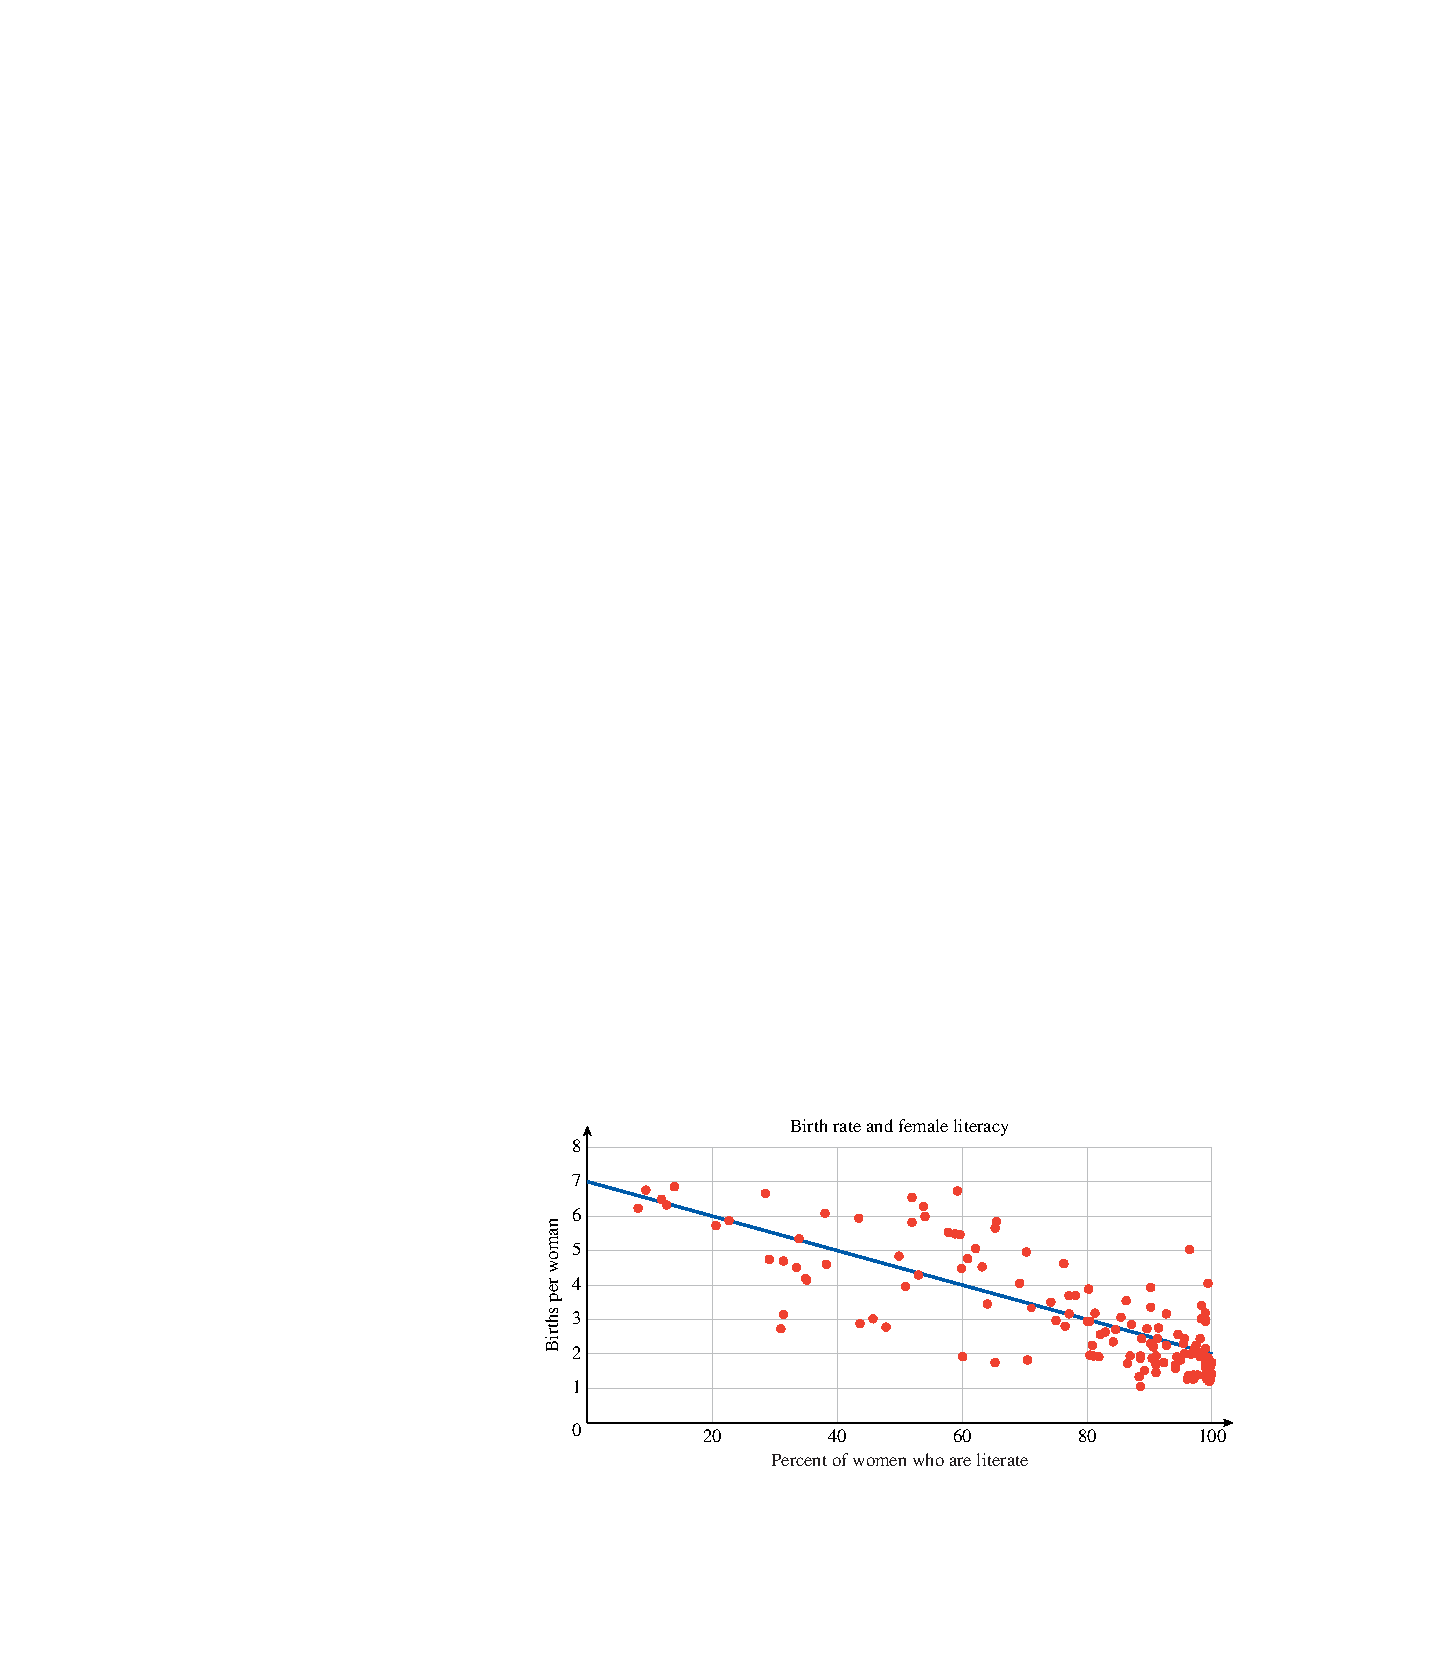
\includegraphics[width=0.100\textwidth,]{images/BirthRateVsFemaleLiteracy.pdf}\end{figure}
\begin{investigation}[Sales on Commission]\label{investigation-1}
Delbert is offered a part-time job selling restaurant equipment. He will be paid \textdollar{}1000 per month plus a 6\% commission on his sales. The sales manager tells Delbert he can expect to sell about \textdollar{}8000 worth of equipment per month. To help him decide whether to accept the job, Delbert does a few calculations.%
\par

                \leavevmode%
\begin{enumerate}
\item\hypertarget{li-1}{}Based on the sales manager’s estimate, what monthly income can Delbert expect from this job? What annual salary would that provide?%
\item\hypertarget{li-2}{}What would Delbert’s monthly salary be if he sold only \textdollar{}5000 of equipment per month? What would his salary be if he sold \textdollar{}10,000 worth per month? Compute monthly incomes for each sales total shown in the table.%
\leavevmode%
\begin{figure}
\centering
\pushValignCaptionBottom[b]{minipage}{.30\textwidth}{%
\centering% horizontal alignment 
\begin{tabular}{AcAcA}\hrulethick
Sales%
&Income%
\tabularnewline\hrulethin
5000&\tabularnewline\hrulethin
8000&\tabularnewline\hrulethin
10,000&\tabularnewline\hrulethin
12,000&\tabularnewline\hrulethin
15,000&\tabularnewline\hrulethin
18,000&\tabularnewline\hrulethin
20,000&\tabularnewline\hrulethin
25,000&\tabularnewline\hrulethin
30,000&\tabularnewline\hrulethin
35,000&\tabularnewline\hrulethin
~&\tabularnewline\hrulethin
~&\tabularnewline\hrulethin
\end{tabular}
}% end body 
{}% caption 
\pushValignCaptionBottom[b]{minipage}{.70\textwidth}{%
\centering% horizontal alignment 
\includegraphics[width=\textwidth,]{images/Investigation1Grid.pdf}}% end body 
{}% caption 
\popValignCaptionBottom
\end{figure}
\item\hypertarget{li-3}{}Plot your data points on a graph, using sales, \(S\), on the horizontal axis and income, \(I\), on the vertical axis, as shown in the figure. Connect the data points to show Delbert’s monthly income for all possible monthly sales totals.%
\item\hypertarget{li-4}{} Add two new data points to the table by reading values from your graph.%
\item\hypertarget{li-5}{} Write an algebraic expression for Delbert’s monthly income, \(I\), in terms of his monthly sales, \(S\). Use the description in the problem to help you:%
\par

                    He will be paid: \textdollar{}1000 . . . plus a 6\% commission on his sales.%
\par
\emph{Income} \(= \fillin{6.818181818181818}\) %
\item\hypertarget{li-6}{}Test your formula from part (5) to see if it gives the same results as those you recorded in the table.%
\item\hypertarget{li-7}{}Use your formula to find out what monthly sales total Delbert would need in order to have a monthly income of \textdollar{}2500.%
\item\hypertarget{li-8}{}Each increase of \textdollar{}1000 in monthly sales increases Delbert’s monthly inbcome by \fillin{6.818181818181818}.%
\item\hypertarget{li-9}{}Summarize the results of your work: In your own words, describe the relationship etween Delbert’s monthly sales and his monthly income. Include in your discussion a description of your graph.%
\end{enumerate}
%
\end{investigation}
\typeout{************************************************}
\typeout{Section 1.1 Linear Models}
\typeout{************************************************}
\section[Linear Models]{Linear Models}\label{LinMod}
\typeout{************************************************}
\typeout{Subsection 1.1.1 Tables, Graphs and Equations}
\typeout{************************************************}
\subsection[Tables, Graphs and Equations]{Tables, Graphs and Equations}\label{subsection-1}
The first step in creating a model is to describe relationships between variables.  In Investigation 1 {$\langle\langle$investigation-commission$\rangle\rangle$}, we analyzed the relationship between Delbert's sales and his income.  Starting from the verbal description of his income, we represented the relationship by a table of values, a graph, and an algebraic equation.  Each of these mathematical tools is useful in a different way.%
\leavevmode%
\begin{enumerate}
\item\hypertarget{li-10}{}A \terminology{table of values} displays specific data points with precise numerical values.%
\item\hypertarget{li-11}{}A \terminology{graph} is a visual display of the data.  It is easier to spot trends and describe the overall behavior of the variables from a graph.%
\item\hypertarget{li-12}{}An \terminology{algebraic equation} is a compact summary of the model.  It can be used to analyze the model and to make predictions%
\end{enumerate}
\par
We begin our study of modeling with some examples of \terminology{linear models}.  In the examples that follow, observe the interplay among the three modeling tools, and how each contributes to the model.%
\begin{example}[]\label{example-Annelise}
Annelise is on vacation at a seaside resort.  She can rent a bicycle from her hotel for \textdollar{}3 an hour, plus a \textdollar{}5 insurance fee.  (A fraction of an hour is charged as the same fraction of \textdollar{}3.)%
\leavevmode%
\begin{enumerate}[label=*\alph**]
\item\hypertarget{li-13}{}Make a table of values showing the cost, \(C\), of renting a bike for various lengths of time, \(t\).%
\item\hypertarget{li-14}{}Plot the points on a graph.  Draw a curve through the data points%
.
                        \item\hypertarget{li-15}{}Write an equation for \(C\) in terms of \(t\).%
\end{enumerate}
\par\medskip\noindent%
\textbf{Solution.}\quad \leavevmode%
\begin{enumerate}[label=*\alph**]
\item\hypertarget{li-16}{}To find the cost, multiply the time by \textdollar{}3, and add the result to the \textdollar{}5 insurance fee.  For example, the cost of a 1-hour bike ride is
                            \begin{align*}
\text{Cost}\amp=(\$5\text{ insurance fee})+(\$3\text{ per hour})\times(\alert{1}\text{ hour})\\
C\amp=5+3(\alert{1})=8
\end{align*}
                            A 1-hour bike ride costs \textdollar{}8.  Record the results in a table, as shown here:%
\leavevmode%
\begin{table}
\centering
\begin{tabular}{AcAcAcAcA}\hrulethick
Length of rental (hours)%
&Cost of rental (dollars)%
&&\((t,C)\)\tabularnewline\hrulethin
1&8&\(C=5+3(\alert{1})\)&\((1,8)\)\tabularnewline\hrulethin
2&11&\(C=5+3(\alert{2})\)&\((2,11)\)\tabularnewline\hrulethin
3&14&\(C=5+3(\alert{3})\)&\((3,14)\)\tabularnewline\hrulethin
\end{tabular}
\end{table}
\item\hypertarget{li-17}{}Each pair of values represents a point on the graph.  The first value gives the horizontal coordinate of the point, and the second value gives the vertical coordinate.  The points lie on a straight line, as shown in the figure.  The line extends infinitely in only one direction, because negative values of \(t\) do not make sense here.%
\leavevmode%
\begin{figure}
\centering
\includegraphics[width=0.50\textwidth,]{images/fig-Annelise-1.pdf}\end{figure}
\item\hypertarget{li-18}{}To find an equation, let \(C\) represent the cost of the rental, and use \(t\) for the number of hours:
        \begin{align*}
\text{Cost}\amp=(\$5\text{ insurance fee})+(\$3\text{ per hour})\times\text{(number of hours)}\\
C\amp=5+3\cdot t=8
\end{align*} %
\end{enumerate}
\end{example}
\begin{example}[]\label{example-6hrbike}
Use the equation \(C=5+3\cdot t\) you found in \hyperref[example-Annelise]{Example~\ref{example-Annelise}} to answer the following questions.  Then show how to find the answers by using the graph.%
\leavevmode%
\begin{enumerate}[label=*\alph**]
\item\hypertarget{li-19}{}How much will it cost Annelise to rent a bicycle for 6 hours?%
\item\hypertarget{li-20}{}How long can Annelise bicycle for \textdollar{}18.50?%
\end{enumerate}
\par\medskip\noindent%
\textbf{Solution.}\quad \leavevmode%
\begin{enumerate}[label=*\alph**]
\item\hypertarget{li-21}{}Substitute \(t=\alert{6}\) into the expression for \(C\) to find \begin{equation*}C=5+3(\alert{6})=23\end{equation*}A 6-hour bike ride will cost \textdollar{}23.  The point \(P\) on the graph in the figure represents the cost of a 6-hour bike ride.  The value on the \(C\)-axis at the same height as point \(P\) is 23, so a 6-hour bike ride costs \textdollar{}23.%
\item\hypertarget{li-22}{}Substitute \(C=\alert{18.50}\) into the equation and solve for \(t\).
        \begin{align*}
\alert{18.50}\amp=5+3t\\
13.50\amp=3t\\
t\amp=4.5
\end{align*}
        For \textdollar{}18.50 Annelise can bicycle for 4½ hours. The point \(Q\)  on the graph represents an \textdollar{}18.50 bike ride.  The value on the \(t\)-axis below point \(Q\) is 4.5, so \textdollar{}18.50 will buy a 4.5 hour bike ride.%
\end{enumerate}
\leavevmode%
\begin{figure}
\centering
\includegraphics[width=0.50\textwidth,]{images/fig1-2.pdf}\end{figure}
\end{example}
\par
In \hyperref[example-6hrbike]{Example~\ref{example-6hrbike}}, notice the different algebraic techniques we used in parts (a) and (b).   In part (a), we were given a value of \(t\) and we \terminology{evaluated the expression}  \(5+3t\) to find \(C\).  In part (b) we were given a value of \(C\) and we \terminology{solved the equation} \(C=5+3t\) to find \(t.\)%
\begin{exercise}\label{exercise-Frank-plants}
 Frank plants a dozen corn seedlings, each 6 inches tall.  With plenty of water and sunlight they will grow approximately 2 inches per day.  Complete the table of values for the height, \(h\), of the seedlings after \(t\) days.%
\leavevmode%
\begin{figure}
\centering
\pushValignCaptionBottom[b]{minipage}{.50\textwidth}{%
\centering% horizontal alignment 
\begin{tabular}{AcAcAcAcAcAcA}\hrulethick
\(t\)&0&5&10&15&20\tabularnewline\hrulethin
\(h\)&&&&&\tabularnewline\hrulethin
\end{tabular}
}% end body 
{}% caption 
\pushValignCaptionBottom[b]{minipage}{.50\textwidth}{%
\centering% horizontal alignment 
\includegraphics[width=\textwidth,]{images/fig-Example2.pdf}}% end body 
{}% caption 
\popValignCaptionBottom
\end{figure}
\leavevmode%
\begin{enumerate}[label=*\alph**]
\item\hypertarget{li-23}{}Write an equation for the height of the seedlings in terms of the number of days since they were planted.%
\item\hypertarget{li-24}{}Graph the equation.%
\end{enumerate}
\end{exercise}
\begin{exercise}\label{exercise-2}
 Use your equation from \hyperref[exercise-Frank-plants]{Exercise~\ref{exercise-Frank-plants}} to answer the questions.  Illustrate each answer on the graph. %
\leavevmode%
\begin{enumerate}[label=*\alph**]
\item\hypertarget{li-25}{} How tall is the corn after 3 weeks? %
\item\hypertarget{li-26}{} How long will it be before the corn is 6 feet tall? %
\end{enumerate}
\end{exercise}
\typeout{************************************************}
\typeout{Subsection 1.1.2 Choosing Scales for the Axes}
\typeout{************************************************}
\subsection[Choosing Scales for the Axes]{Choosing Scales for the Axes}\label{subsection-2}
To draw a useful graph, we must choose appropriate scales for the axes.  They must extend far enough to show the values of the variables, and the tick marks should be equally spaced.  Usually no more than 10 or 15 tick marks are needed.%
\begin{example}[]\label{example-home-price}
In 1990, the median home price in the US was \textdollar{}92,000.  The median price increased by about \textdollar{}4700 per year over the next decade.
        \leavevmode%
\begin{enumerate}[label=*\alph**]
\item\hypertarget{li-27}{} Make a table of values showing the median price of a house in 1990, 1994, 1998, and 2000.%
\item\hypertarget{li-28}{} Choose suitable scales for the axes and plot the values you found in part (a) on a graph. Use \(t\), the number of years since 1990, on the horizontal axis and the price of the house, \(P\), on the vertical axis.  Draw a curve through the points.%
\item\hypertarget{li-29}{} Write an equation that expresses \(P\) in terms of \(t\).%
\item\hypertarget{li-30}{} How much did the price of the house increase from 1990 to 1996?  Illustrate the increase on your graph.%
\end{enumerate}

    %
\par\medskip\noindent%
\textbf{Solution.}\quad \leavevmode%
\begin{enumerate}[label=*\alph**]
\item\hypertarget{li-31}{}In 1990 the median price was \textdollar{}92,000.  Four years later, in 1994, the price had increased by \(\alert{4}(4700)=18,800\) dollars, so
        \begin{equation*}P=92,000+\alert{4}(4700)=110,800\end{equation*}
        In 1998 the price had increased by \(\alert{8}(4700)=37,600\)  dollars, so
        \begin{equation*}P=92,000+\alert{8}(4700)-129,600\end{equation*}
        You can verify the price of the house in 2000 by a similar calculation.%
\leavevmode%
\begin{table}
\centering
\begin{tabular}{AcAcAcA}\hrulethick
Year%
&Price of House)%
&\((t,P)\)\tabularnewline\hrulethin
1990&92,000&\((0, 92,000)\)\tabularnewline\hrulethin
1994&110,800&\((4, 110,800)\)\tabularnewline\hrulethin
1998&129,600&\((8, 129,600)\)\tabularnewline\hrulethin
2000&139,000&\((10, 139,000)\)\tabularnewline\hrulethin
\end{tabular}
\end{table}
\item\hypertarget{li-32}{}Let \(t\) stand for the number of years since 1990, so that \(t=0\) in 1990, \(t=4\) in 1994, and so on.  To choose scales for the axes,
             look at the values in the table.  For this graph we scale the horizontal axis, or \(t\)-axis, in 1-year intervals and the vertical axis, or \(P\)-axis, for \textdollar{}90,000 to \textdollar{}140,000 in intervals of \textdollar{}5,000. The points in Figure 1. lie on a straight line.%
\item\hypertarget{li-33}{}Look back at the calculations in part (a).  The price of the house started at \textdollar{}92,000 in 1990 and increased by \(t \times 4700\) dollars after \(t\) years.  Thus,
            \begin{equation*}P=92,000+4700t\end{equation*}%
\item\hypertarget{li-34}{}Find the points on the graph corresponding to 1990 and 1996.  These points lie above \(t=0\) and \(t=6\) on the \(t\)-axis.  Now find the values on the \(P\)-axis corresponding to the two points.  The values are \(P=92,000\) in 1990 and \(P=120,200\) in 1996.  The increase in price is the difference of the two \(P\)-values.
            \begin{align*}
\text{increase in price}\amp=120,200-92,000
                \\
\amp=28,200
\end{align*}  
            The price of the home increased \textdollar{}28,200 between 1990 and 1996.  This increase is indicated by the arrows in \hyperref[fig-median-house]{Figure~\ref{fig-median-house}} [ref].%
\leavevmode%
\begin{figure}
\centering
\includegraphics[width=0.50\textwidth,]{images/fig1-3.pdf}\caption{\label{fig-median-house}}
\end{figure}
\end{enumerate}
\end{example}
\par
The graphs in the preceding examples are \terminology{increasing graphs}.  As we move along the graph from left to right (in the direction of increasing \(t\) ), the second coordinate increases as well.  Try Exercise 3, which illustrates a \terminology{decreasing graph}.%
\begin{exercise}\label{exercise-Silver-Lake}
Silver Lake has been polluted by industrial waste products.  The concentration of toxic chemicals in the water is currently 285 parts per million (ppm).  Local environmental officials would like to reduce the concentration by 15 ppm each year%
\leavevmode%
\begin{enumerate}[label=*\alph**]
\item\hypertarget{li-35}{}Complete the table of values showing the desired concentration, \(C,\)~ of toxic chemicals \(t\) years from now.  For each \(t\)-value, calculate the corresponding value for \(C\).  Write your answers as ordered pairs.%
\leavevmode%
\begin{table}
\centering
\begin{tabular}{AcAcAcAcA}\hrulethick
\(t\)%
&\(C\)%
&&\((t,C)\)\tabularnewline\hrulethin
0&&\(C=285-150(\alert{0})\)&\((0, ~~~~ )\)\tabularnewline\hrulethin
5&&\(C=285-150(\alert{5})\)&\((5, ~~~~ )\)\tabularnewline\hrulethin
10&&\(C=285-150(\alert{10})\)&\((10, ~~~~ )\)\tabularnewline\hrulethin
15&&\(C=285-150(\alert{15})\)&\((15, ~~~~ )\)\tabularnewline\hrulethin
\end{tabular}
\end{table}
\item\hypertarget{li-36}{}To choose scales for the axes, notice that the value of \(C\) starts at 285 and decreases from there.  We'll scale the vertical axis up to 300, and use 10 tick marks at intervals of 30.  Graph the ordered pairs on the grid, and connect them with a straight line. Extend the graph until it reaches the horizontal axis, but no farther.  Points with negative \(C\)-coordinates have no meaning for the problem.%
\item\hypertarget{li-37}{}Write an equation for the concentration, \(C\), of toxic chemicals \(t\) years from now.  (Hint:  The concentration is initially 8 ppm, and we subtract 15 ppm for each year that passes, or \(15 \times t\).)%
\includegraphics[width=0.50\textwidth,]{images/fig-Exercise3.pdf}\end{enumerate}
\end{exercise}
\begin{remark}[\includegraphics[width=0.8\textwidth,]{images/icon-GC.jpg}Graphing an Equation]\label{remark-1}
We can use a graphing calculator to graph an equation. On most calculators, we follow three steps.%
\par
To Graph an Equation:%
\leavevmode%
\begin{enumerate}
\item\hypertarget{li-38}{}Press \lstinline?Y=? and enter the equation you wish to graph.%
\item\hypertarget{li-39}{}Press \lstinline?WINDOW? and select a suitable graphing window.%
\item\hypertarget{li-40}{}Press \lstinline?GRAPH?%
\end{enumerate}
\end{remark}
\begin{example}[\includegraphics[width=0.8\textwidth,]{images/icon-GC.jpg}Using a Graphing Calculator]\label{graphing-calculator}
In \hyperref[example-home-price]{Example~\ref{example-home-price}}, we found the equation \(P = 92,000 + 4700t\) for the median price of a house \(t\) years after 1990. Graph this equation on a calculator.%
\par\medskip\noindent%
\textbf{Solution.}\quad 
            To begin, we press \lstinline?Y=? and enter
        %
\par

             \begin{equation*}Y1 = 92,000 + 4700X\end{equation*}
        %
\par
For this graph, we’ll use the grid in \hyperref[example-home-price]{Example~\ref{example-home-price}} for our window settings, so we press \lstinline?WINDOW? and enter
        %
\leavevmode%
\begin{table}
\centering
\begin{tabular}{lll}
Xmin\(=0\)&&Xmax\(=10\)\tabularnewline[0pt]
Ymin\(=90,000\)&&Ymax\(=140,000\)
\end{tabular}
\end{table}
\par

        Finally, we press \lstinline?GRAPH?. The calculator’s graph is shown in \hyperref[fig-GC-house-price]{Figure~\ref{fig-GC-house-price}}.%
\leavevmode%
\begin{figure}
\centering
\includegraphics[width=0.50\textwidth,]{images/fig-GC-house-price.pdf}\caption{\label{fig-GC-house-price}}
\end{figure}
\end{example}
\begin{exercise}\label{exercise-gc}
\leavevmode%
\begin{enumerate}[label=*\alph**]
\item\hypertarget{li-41}{}Solve the equation \(2y − 1575 = 45x\) for \(y\) in terms of \(x\).%
\item\hypertarget{li-42}{}Graph the equation on a graphing calculator. Use the window
        \leavevmode%
\begin{table}
\centering
\begin{tabular}{lllll}
Xmin\(=-50\)&&Xmax\(=50\)&&Xscl\(=5\)\tabularnewline[0pt]
Ymin\(=-500\)&&Ymax\(=1000\)&&Yscl\(=100\)
\end{tabular}
\end{table}
%
\item\hypertarget{li-43}{}Sketch the graph on paper. Use the window settings to choose appropriate scales for the axes.%
\end{enumerate}
\end{exercise}
\typeout{************************************************}
\typeout{Subsection 1.1.3 Linear Equations}
\typeout{************************************************}
\subsection[Linear Equations]{Linear Equations}\label{subsection-3}
All the models in these examples have equations with a similar form:  \begin{equation*}y=\text{(starting value)}+\text{(rate of change)}\cdot x\end{equation*}
(We'll talk more about rate of change in Section 1.4.)  Their graphs were all portions of straight lines.  For this reason such equations are called  \terminology{linear equations}.  The order of the terms in the equation does not matter.  For example, the equation in Example 1, \begin{equation*}C=5+3t\end{equation*} can be written equivalently as \begin{equation*}-3t+C=5\end{equation*} and the equation in Example 3, \begin{equation*}P=92,000+4700t\end{equation*} can be written as \begin{equation*}-4700+P=92,000\end{equation*} 
This form of a linear equation, \begin{equation*}Ax+By=C\end{equation*} is called the \terminology{general form}.%
\begin{mdframed}[style=assemblage]%
\noindent\textbf{\large General Form for a Linear Equation}\label{assemblage-1}\par\medskip
The graph of any equation \begin{equation*}Ax+By=C\end{equation*} where \(A\) and \(B\) are not both equal to zero, is a straight line.%
\end{mdframed}
\begin{example}[]\label{example-advertising}
The manager at Albert's Appliances has \textdollar{}3000 to spend on advertising for the next fiscal quarter.  A 30-second spot on television costs \textdollar{}150 per broadcast, and a 30-second radio ad costs \textdollar{}50.%
\leavevmode%
\begin{enumerate}[label=*\alph**]
\item\hypertarget{li-44}{}The manager decides to buy \(x\) television ads and \(y\) radio ads.  Write an equation relating \(x\) and \(y\).%
\item\hypertarget{li-45}{}Make a table of values showing several choices for \(x\) and \(y\).%
\item\hypertarget{li-46}{}Plot the points from your table, and graph the equation.%
\end{enumerate}
\par\medskip\noindent%
\textbf{Solution.}\quad \leavevmode%
\begin{enumerate}[label=*\alph**]
\item\hypertarget{li-47}{}Each television ad costs \textdollar{}150, so ads will cost \textdollar{}150.  Similarly, radio ads will cost \textdollar{}50.  The manager has \textdollar{}3000 to spend, so the sum of the costs must be \textdollar{}3000.  Thus, \begin{equation*}150x+50y=3000\end{equation*}%
\item\hypertarget{li-48}{}Choose some values of \(x\), and solve the equation for the corresponding value of \(y\)  For example, if \(x=\alert{10}\) then
               \begin{align*}
150(10)+50y\amp=300\\
1500+50y\amp=3000\\
50y\amp=1500\\
y\amp=30
\end{align*}
                If the manager buys 10 television ads, she can also buy 30 radio ads.  You can verify the other entries in the table.%
\leavevmode%
\begin{table}
\centering
\begin{tabular}{AcAcAcAcAcA}\hrulethick
\(x\)&8&10&12&14\tabularnewline\hrulethin
\(y\)&&&&\tabularnewline\hrulethin
\end{tabular}
\end{table}
\item\hypertarget{li-49}{}Plot the points from the table.  All the solutions lie on a straight line, as shown in \hyperref[fig-example-advertising]{Figure~\ref{fig-example-advertising}}
.
        \leavevmode%
\begin{figure}
\centering
\includegraphics[width=0.50\textwidth,]{images/fig-example-advertising.pdf}\caption{\label{fig-example-advertising}}
\end{figure}
%
\end{enumerate}
\end{example}
\begin{exercise}\label{exercise-crops}
In central Nebraska, each acre of corn requires 25 acre-inches of water per year, and each acre of winter wheat requires 18 acre-inches of water.             (An acre-inch is the amount of water needed to cover one acre of land to a depth of one inch.)  A farmer can count on 9000 acre-inches of water for the coming year.  (Source:  Institute of Agriculture and Natural Resources, University of Nebraska)
    \leavevmode%
\begin{enumerate}[label=*\alph**]
\item\hypertarget{li-50}{}Write an equation relating the number of acres of corn, \(x\), and the number of acres of wheat, \(y\), that the farmer can plant.%
\item\hypertarget{li-51}{}Complete the table.%
\leavevmode%
\begin{table}
\centering
\begin{tabular}{AcAcAcAcAcA}\hrulethick
\(x\)&50&100&150&200\tabularnewline\hrulethin
\(y\)&&&&\tabularnewline\hrulethin
\end{tabular}
\end{table}
\end{enumerate}
%
\end{exercise}
\typeout{************************************************}
\typeout{Subsection 1.1.4 Intercepts}
\typeout{************************************************}
\subsection[Intercepts]{Intercepts}\label{subsection-4}
\leavevmode%
\begin{figure}
\centering
\pushValignCaptionBottom[b]{minipage}{.50\textwidth}{%
\centering% horizontal alignment 
\includegraphics[width=\textwidth,]{images/fig-intercepts.pdf}}% end body 
{\captionof{figure}{\label{fig-intercepts}}
}% caption 
\pushValignCaptionBottom[b]{minipage}{.50\textwidth}{%
\parbox{\textwidth}{%
% horizontal alignment 
Consider the graph of the equation \begin{equation*}3x-4y=12\end{equation*} shown in \hyperref[fig-intercepts]{Figure~\ref{fig-intercepts}}. The points where the graph crosses the axes are called the \terminology{intercepts} of the graph. The coordinates of these points are easy to find.  The \(y\)-coordinate of the \(x\)-intercept is zero, so we set \(y=\alert{0}\) in the equation to get \begin{align*}
3(\alert{0})-4x\amp=12\\
x=-3
\end{align*} 
        }%
}% end body 
{}% caption 
\popValignCaptionBottom
\end{figure}
The \(x\)-intercept is the point\((-3,0)\). Also, the \(x\)-coordinate of the \(y\)-intercept is zero, so we set \(x=\alert{0}\) in the equation to get \begin{gather*}
3y-4(\alert{0})=12\\
y=4
\end{gather*}  The \(y\)-intercept is \((0,4)\).%
\begin{mdframed}[style=assemblage]%
\noindent\textbf{\large Intercepts of a Graph}\label{assemblage-2}\par\medskip
The points where a graph crosses the axes are called the \terminology{intercepts of the graph}.
        \leavevmode%
\begin{enumerate}
\item\hypertarget{li-52}{}To find the \(y\)-intercept, set \(x=0\) and solve for \(y\).%
\item\hypertarget{li-53}{}To find the \(x\)-intercept, set \(y=0\) and solve for \(x\)%
\end{enumerate}
%
\end{mdframed}
\par

      The intercepts of a graph tell us something about the situation it models.  
    %
\begin{example}[]\label{example-intercepts}
\leavevmode%
\begin{enumerate}[label=*\alph**]
\item\hypertarget{li-54}{}
        Find the intercepts of the graph in \hyperref[exercise-Silver-Lake]{Exercise~\ref{exercise-Silver-Lake}}, about the pollution in Silver Lake.
    \item\hypertarget{li-55}{}What do the intercepts tell us about the problem?
    \end{enumerate}
\par\medskip\noindent%
\textbf{Solution.}\quad \leavevmode%
\begin{enumerate}[label=*\alph**]
\item\hypertarget{li-56}{}An equation for the concentration of toxic chemicals is \begin{equation*}C=285-15t\end{equation*} To find the \(C\)-intercept, set \(t\) equal to zero. 

            \begin{equation*}C=285-15(0)=285\end{equation*}
            The \(C\)-intercept is the point \((0, 285)\), or simply 285.  To find the \(t\)-intercept, set \(C\) equal to zero and solve for \(t\).
            
                \begin{align*}
                \alert{0}\&=285-15t \&\&\text{Add }15t \text{ to both sides.}\textbackslash{}\textbackslash{}
                15t\&=285  \&\&\text{Divide both sides by 15.}\textbackslash{}\textbackslash{}
                t\&=19   \&\& 
                \end{align*}
            %


        The \(t\)-intercept is the point \((19,0)\), or simply \(19\).%
\item\hypertarget{li-57}{}The \(C\)-intercept represents the concentration of toxic chemicals in Silver Lake now:  When  \(t=0\), \(C=285\),  so the concentration is currently \(285\) ppm.  The \(t\)-intercept represents the number of years it will take for the concentration of toxic chemicals to drop to zero:  When \(C=0\), \(t=19\),  so it will take \(19\) years for the pollution to be eliminated entirely.%
\end{enumerate}
\end{example}
\begin{exercise}\label{exercise-6}
\leavevmode%
\begin{enumerate}[label=*\alph**]
\item\hypertarget{li-58}{}Find the intercepts of the graph in \hyperref[example-advertising]{Example~\ref{example-advertising}}, about the advertising budget for Albert’s Appliances: \(150x + 50y = 3000\).%
\item\hypertarget{li-59}{}What do the intercepts tell us about the problem?%
\end{enumerate}
\end{exercise}
\typeout{************************************************}
\typeout{Subsection 1.1.5 Intercept Method for Graphing Lines}
\typeout{************************************************}
\subsection[Intercept Method for Graphing Lines]{Intercept Method for Graphing Lines}\label{subsection-5}
Because we really only need two points to graph a linear equation, we might as well find the intercepts first and use them to draw the graph. The values of the intercepts will also help us choose suitable scales for the axes. It is always a good idea to find a third point as a check.
    %
\begin{example}[]\label{intercepts}
\leavevmode%
\begin{enumerate}[label=*\alph**]
\item\hypertarget{li-60}{}Find the \(x\)- and \(y\)-intercepts of the graph of \(150x − 180y = 9000\).%
\item\hypertarget{li-61}{}Use the intercepts to graph the equation. Find a third point as a check.%
\end{enumerate}
\par\medskip\noindent%
\textbf{Solution.}\quad \leavevmode%
\begin{enumerate}[label=*\alph**]
\item\hypertarget{li-62}{}To find the \(x\)-intercept, set \(y = \alert{0}\).
            %
\par

                \begin{align*}
                150x-18(\alert{0})\&=9000 \&\&\text{Simpify.}\textbackslash{}\textbackslash{}
                150x\&=9000  \&\&\text{Divide both sides by 150.}\textbackslash{}\textbackslash{}
                x\&=60   \&\& 
                \end{align*}
            %
\par
The \(x\)-intercept is the point \((60, 0)\). To find the \(y\)-intercept, set \(x = \alert{0}\).%
\par

                \begin{align*}
                150(\alert{0})-18y\&=9000 \&\&\text{Simpify.}\textbackslash{}\textbackslash{}
                -180y\&=9000  \&\&\text{Divide both sides by } -180\text{.}\textbackslash{}\textbackslash{}
                y\&=-50   \&\& 
                \end{align*}
            %
\par
The \(y\)-intercept is the point \((0, −50)\).%
\item\hypertarget{li-63}{}Scale both axes in intervals of 10 and then plot the two intercepts, \((60, 0)\) and \((0, −50)\). Draw the line through them, as shown in \hyperref[fig-example-graph-intercepts]{Figure~\ref{fig-example-graph-intercepts}}. Now find another point and check that it lies on this line. We choose \(x = \alert{20}\) and solve for \(y\).
            \begin{gather*}
150(\alert{20}) −180y = 9000\\
3000 −180y = 9000\\
−180y = 6000\\
y =−33.\overline{3}
\end{gather*}

            Plot the point \((20, −33\frac{1}{3})\). Because this point lies on the line, we can be reasonably confident that our graph is correct. 
            \leavevmode%
\begin{figure}
\centering
\includegraphics[width=0.50\textwidth,]{images/fig-example-graph-intercepts.pdf}\caption{\label{fig-example-graph-intercepts}}
\end{figure}

            %
\end{enumerate}
\end{example}
\begin{remark}[\includegraphics[width=0.8\textwidth,]{images/icon-GC.jpg}Choosing a Graphing Window]\label{remark-2}
Knowing the intercepts can also help us choose a suitable window on a graphing calculator. We would like the window to be large enough to show the intercepts. For the graph in \hyperref[fig-example-graph-intercepts]{Figure~\ref{fig-example-graph-intercepts}}, we can enter the equation \begin{equation*}Y = (9000 −150X)/ −180\end{equation*}
    in the window
        \leavevmode%
\begin{table}
\centering
\begin{tabular}{lll}
Xmin\(=-20\)&&Xmax\(=70\)\tabularnewline[0pt]
Ymin\(=-70\)&&Ymax\(=30\)
\end{tabular}
\end{table}

    %
\end{remark}
\begin{mdframed}[style=assemblage]%
\noindent\textbf{\large To Graph a Line Using the Intercept Method:}\label{assemblage-3}\par\medskip

    \leavevmode%
\begin{enumerate}[label=*\arabic**]
\item\hypertarget{li-64}{}Find the intercepts of the line.%
\begin{enumerate}[label=++\alph*]
\item\hypertarget{li-65}{}To find the \(x\)-intercept, set \(y=0\) and solve for \(x\).%
\item\hypertarget{li-66}{}To find the \(y\)-intercept, set \(x = 0\) and solve for \(y\).%
\end{enumerate}
\item\hypertarget{li-67}{}Plot the intercepts.%
\item\hypertarget{li-68}{}Choose a value for \(x\) and find a third point on the line.%
\item\hypertarget{li-69}{}Draw a line through the points.%
\end{enumerate}
%
\end{mdframed}
\begin{exercise}\label{exercise-intercepts}
\leavevmode%
\begin{enumerate}[label=*\alph**]
\item\hypertarget{li-70}{}In \hyperref[exercise-crops]{Exercise~\ref{exercise-crops}}, you wrote an equation about crops in Nebraska. Find the intercepts of the graph.%
\item\hypertarget{li-71}{}Use the intercepts to help you choose appropriate scales for the axes, and then graph the equation.%
\item\hypertarget{li-72}{}What do the intercepts tell us about the problem?%
\end{enumerate}
\end{exercise}
\par
The examples in this section model simple linear relationships between two variables.
Such relationships, in which the value of one variable is determined by the value of the
other, are called \terminology{functions}. We will study various kinds of functions throughout the course.%
\typeout{************************************************}
\typeout{Section 1.2 Functions}
\typeout{************************************************}
\section[Functions]{Functions}\label{functions}
\typeout{************************************************}
\typeout{Subsection 1.2.1 Definition of Function}
\typeout{************************************************}
\subsection[Definition of Function]{Definition of Function}\label{subsection-6}

    We often want to predict values of one variable from the values of a related variable. For example, when a physician prescribes a drug in a certain dosage, she needs to know how long the dose will remain in the bloodstream. A sales manager needs to know how the price of his product will affect its sales. A \terminology{function} is a special type of relationship between variables that allows us to make such predictions.%
\par

    Suppose it costs \textdollar{}800 for flying lessons, plus \textdollar{}30 per hour to rent a plane. If we let \(C\) represent the total cost for t hours of flying lessons, then
    \begin{equation*}C=800+305t ~~~~ (t\ge 0)\end{equation*}
    Thus, for example
%
\leavevmode%
\begin{table}
\centering
\begin{tabular}{rll}
when&\(t=\alert{0}\),&\(C=800+30(\alert{0})=800\)\tabularnewline[0pt]
when&\(t=\alert{4}\),&\(C=800+30(\alert{4})=920\)\tabularnewline[0pt]
when&\(t=\alert{10}\),&\(C=800+30(\alert{10})=1100\)
\end{tabular}
\end{table}
\par

    The variable \(t\) is called the \terminology{input} or \terminology{independent} variable, and \(C\) is the \terminology{output} or \terminology{dependent} variable, because its values are determined by the value of \(t\). We can display the relationship between two variables by a table or by ordered pairs. The input variable is the first component of the ordered pair, and the output variable is the second component.
%
\leavevmode%
\begin{table}
\centering
\begin{tabular}{AcAcAcA}\hrulethick
\(t\)&\(C\)&\((t,C)\)\tabularnewline\hrulethin
\(0\)&\(800\)&\((0, 800)\)\tabularnewline\hrulethin
\(4\)&\(920\)&\((4, 920)\)\tabularnewline\hrulethin
\(10\)&\(1100\)&\((10,1100)\)\tabularnewline\hrulethin
\end{tabular}
\end{table}
\par

    For this relationship, we can find the value \(C\) of associated with any given value of \(t\). All we have to do is substitute the value of \(t\) into the equation and solve for \(C\). The result has no ambiguity: Only one value for \(C\) corresponds to each value of \(t\). This type of relationship between variables is called a \terminology{function}. In general, we make the following definition.
%
\begin{mdframed}[style=assemblage]%
\noindent\textbf{\large Definition of Function}\label{assemblage-4}\par\medskip
A \terminology{function} is a relationship between two variables for which a unique value of the \terminology{output} variable can be determined from a value of the \terminology{input} variable.
    %
\end{mdframed}
\par

    What distinguishes functions from other variable relationships? The definition of a function calls for a \emph{unique value}—that is, \emph{exactly one value} of the output variable corresponding to each value of the input variable. This property makes functions useful in applications because they can often be used to make predictions.
%
\begin{example}[]\label{example-functions}

        \leavevmode%
\begin{enumerate}[label=*\alph**]
\item\hypertarget{li-73}{}The distance, \(d\), traveled by a car in 2 hours is a function of its speed, \(r\). If we know the speed of the car, we can determine the distance it travels by the formula \(d = r \cdot 2\).%
\item\hypertarget{li-74}{}The cost of a fill-up with unleaded gasoline is a function of the number of gallons purchased. The gas pump represents the function by displaying the corresponding values of the input variable (number of gallons) and the output variable (cost).%
\item\hypertarget{li-75}{}Score on the Scholastic Aptitude Test (SAT) is not a function of score on an IQ test, because two people with the same score on an IQ test may score differently on the SAT; that is, a person’s score on the SAT is not uniquely determined by his or her score on an IQ test.%
\end{enumerate}


    %
\end{example}
\begin{exercise}\label{exercise-functions}

    \leavevmode%
\begin{enumerate}[label=*\alph**]
\item\hypertarget{li-76}{}As part of a project to improve the success rate of freshmen, the counseling department studied the grades earned by a group of students in English and algebra. Do you think that a student’s grade in algebra is a function of his or her grade in English? Explain why or why not.%
\item\hypertarget{li-77}{}Phatburger features a soda bar, where you can serve your own soft drinks in any size. Do you think that the number of calories in a serving of Zap Kola is a function of the number of fluid ounces? Explain why or why not.%
\end{enumerate}
%
\end{exercise}
\typeout{************************************************}
\typeout{Subsection 1.2.2 Functions Defined by Tables}
\typeout{************************************************}
\subsection[Functions Defined by Tables]{Functions Defined by Tables}\label{subsection-7}
When we use a table to describe a function, the first variable in the table (the left column of a vertical table or the top row of a horizontal table) is the input variable, and the second variable is the output. We say that the output variable is a function of the input.%
\begin{example}[]\label{example-table-functions}
\leavevmode%
\begin{enumerate}[label=*\alph**]
\item\hypertarget{li-78}{}\hyperref[table-auto-sales]{Table~\ref{table-auto-sales}} shows data on sales compiled over several years by the accounting office for Eau Claire Auto Parts, a division of Major Motors. In this example, the year is the input variable, and total sales is the output. We say that total sales, \(S\), is a function of \(t\).%
\leavevmode%
\begin{table}
\centering
\begin{tabular}{AcAcA}\hrulethick
Year \((t)\)%
&Total sales \((S)\)%
\tabularnewline\hrulethin
2000&\textdollar{}612,000\tabularnewline\hrulethin
2001&\textdollar{}663,000\tabularnewline\hrulethin
2002&\textdollar{}692,000\tabularnewline\hrulethin
2003&\textdollar{}749,000\tabularnewline\hrulethin
2004&\textdollar{}904,000\tabularnewline\hrulethin
\end{tabular}
\caption{\label{table-auto-sales}}
\end{table}
\item\hypertarget{li-79}{}\hyperref[table-postage]{Table~\ref{table-postage}} gives the cost of sending printed material by first-class mail in 2016. %
\leavevmode%
\begin{table}
\centering
\begin{tabular}{AcAcA}\hrulethick
Weight in ounces \((w)\)&Postage \((P)\)\tabularnewline\hrulethin
\(0 \lt w \le 1 \)&\textdollar{}0.47\tabularnewline\hrulethin
\(1 \lt w \le 2 \)&\textdollar{}0.68\tabularnewline\hrulethin
\(2 \lt w \le 3 \)&\textdollar{}0.89\tabularnewline\hrulethin
\(3 \lt w \le 4 \)&\textdollar{}1.10\tabularnewline\hrulethin
\(4 \lt w \le 5 \)&\textdollar{}1.31\tabularnewline\hrulethin
\(5 \lt w \le 6 \)&\textdollar{}1.52\tabularnewline\hrulethin
\(6 \lt w \le 7 \)&\textdollar{}1.73\tabularnewline\hrulethin
\end{tabular}
\caption{\label{table-postage}}
\end{table}
\par
If we know the weight of the article being shipped, we can determine the required postage from \hyperref[table-postage]{Table~\ref{table-postage}}. For instance, a catalog weighing 4.5 ounces would require \textdollar{}1.31 in postage. In this example, \(w\) is the input variable and \(p\) is the output variable. We say that \(p\) \emph{is a function of} \(w\).%
\item\hypertarget{li-80}{}\hyperref[table-cholesterol]{Table~\ref{table-cholesterol}} records the age and cholesterol count for 20 patients tested in a hospital survey.%
\leavevmode%
\begin{table}
\centering
\begin{tabular}{AcAcAcAcAcA}\hrulethick
Age%
&Cholesterol count%
&&Age%
&Cholesterol count%
\tabularnewline\hrulethin
53&217&&\(\alert{51}\)&\(\alert{209}\)\tabularnewline\hrulethin
48&232&&53&241\tabularnewline\hrulethin
55&198&&49&186\tabularnewline\hrulethin
56&238&&\(\alert{51}\)&\(\alert{216}\)\tabularnewline\hrulethin
\(\alert{51}\)&\(\alert{227}\)&&57&208\tabularnewline\hrulethin
52&264&&52&248\tabularnewline\hrulethin
53&195&&50&214\tabularnewline\hrulethin
47&203&&56&271\tabularnewline\hrulethin
48&212&&53&193\tabularnewline\hrulethin
50&234&&48&172\tabularnewline\hrulethin
\end{tabular}
\caption{\label{table-cholesterol}}
\end{table}
\par
According to these data, cholesterol count is \emph{not} a function of age, because several patients who are the same age have different cholesterol levels. For example, three different patients are 51 years old but have cholesterol counts of 227, 209, and 216, respectively. Thus, we cannot determine a \emph{unique} value of the output variable (cholesterol count) from the value of the input variable (age). Other factors besides age must influence a person’s cholesterol count.%
\end{enumerate}
\end{example}
\begin{exercise}\label{exercise-9}
Decide whether each table describes \(y\) as a function of \(x\). Explain your choice.
    \leavevmode%
\begin{enumerate}[label=*\alph**]
\item\hypertarget{li-81}{}\leavevmode%
\begin{table}
\centering
\begin{tabular}{AcAcAcAcAcAcAcAcAcA}\hrulethick
\(x\)%
&3.5%
&2.0%
&2.5%
&3.5%
&2.5%
&4.0%
&2.5%
&3.0%
\tabularnewline\hrulethin
\(y\)%
&2.5%
&3.0%
&2.5%
&4.0%
&3.5%
&4.0%
&2.0%
&2.5%
\tabularnewline\hrulethin
\end{tabular}
\end{table}
\item\hypertarget{li-82}{}\leavevmode%
\begin{table}
\centering
\begin{tabular}{AcAcAcAcAcAcAcAcA}\hrulethick
\(x\)%
&\(-3\)%
&\(-2\)%
&\(-1\)%
&\(0\)%
&\(1\)%
&\(2\)%
&\(3\)%
\tabularnewline\hrulethin
\(y\)%
&\(17\)%
&\(3\)%
&\(0\)%
&\(-1\)%
&\(0\)%
&\(3\)%
&\(17\)%
\tabularnewline\hrulethin
\end{tabular}
\end{table}
\end{enumerate}
\end{exercise}
\typeout{************************************************}
\typeout{Subsection 1.2.3 Functions Defined by Graphs}
\typeout{************************************************}
\subsection[Functions Defined by Graphs]{Functions Defined by Graphs}\label{subsection-8}

    A graph may also be used to define one variable as a function of another. The input variable is displayed on the horizontal axis, and the output variable on the vertical axis.
%
\begin{example}[]\label{example-sun-hours}
\hyperref[fig-sun-hours]{Figure~\ref{fig-sun-hours}}  shows the number of hours, \(H\), that the sun is above the horizon in Peoria, Illinois, on day \(t\), where January 1 corresponds to \(t = 0\).%
\leavevmode%
\begin{figure}
\centering
\pushValignCaptionBottom[b]{minipage}{.50\textwidth}{%
% horizontal alignment 
\parbox{\textwidth}{%
% horizontal alignment 
\leavevmode%
\begin{enumerate}[label=*\alph**]
\item\hypertarget{li-83}{}Which variable is the input, and which is the output?%
\item\hypertarget{li-84}{}Approximately how many hours of sunlight are there in Peoria on day 150?%
\item\hypertarget{li-85}{}On which days are there 12 hours of sunlight?%
\item\hypertarget{li-86}{}What are the maximum and minimum values of \(H\), and when do these valuesoccur?%
\end{enumerate}
}%
}% end body 
{}% caption 
\pushValignCaptionBottom[b]{minipage}{.50\textwidth}{%
\centering% horizontal alignment 
\includegraphics[width=\textwidth,]{images/fig-sun-hours.pdf}}% end body 
{\captionof{figure}{\label{fig-sun-hours}}
}% caption 
\popValignCaptionBottom
\end{figure}
\par\medskip\noindent%
\textbf{Solution.}\quad \leavevmode%
\begin{enumerate}[label=*\alph**]
\item\hypertarget{li-87}{}The input variable, \(t\), appears on the horizontal axis. The number of daylight hours, \(H\), is a function of the date. The output variable appears on the vertical axis.%
\item\hypertarget{li-88}{}The point on the curve where \(t = 150\) has \(H \approx 14.1\), so Peoria gets about 14.1 hours of daylight when \(t = 150\), which is at the end of May.%
\item\hypertarget{li-89}{}\(H = 12\) at the two points where \(t \approx 85\) (in late March) and \(t \approx 270\) (late September).%
\item\hypertarget{li-90}{}The maximum value of 14.4 hours occurs on the longest day of the year, when \(t \approx 170\), about three weeks into June. The minimum of 9.6 hours occurs on the shortest day, when \(t \approx 355\), about three weeks into December.%
\end{enumerate}
\end{example}
\begin{exercise}\label{exercise-LA-marathon}
\hyperref[fig-LA-marathon]{Figure~\ref{fig-LA-marathon}}  shows the elevation in feet, \(a\), of the Los Angeles Marathon course at a distance \(d\) miles into the race. (Source: \emph{Los Angeles Times}, March 3, 2005)
    \leavevmode%
\begin{figure}
\centering
\includegraphics[width=0.100\textwidth,]{images/fig-LA-marathon.pdf}\caption{\label{fig-LA-marathon}}
\end{figure}
\leavevmode%
\begin{enumerate}[label=*\alph**]
\item\hypertarget{li-91}{}Which variable is the input, and which is the output?%
\item\hypertarget{li-92}{}What is the elevation at mile 20?%
\item\hypertarget{li-93}{}At what distances is the elevation 150 feet?%
\item\hypertarget{li-94}{}What are the maximum and minimum values of \(a\), and when do these values occur?%
\item\hypertarget{li-95}{}The runners pass by the Los Angeles Coliseum at about 4.2 miles into the race. What is the elevation there?%
\end{enumerate}
\end{exercise}
\typeout{************************************************}
\typeout{Subsection 1.2.4 Functions Defined by Equations}
\typeout{************************************************}
\subsection[Functions Defined by Equations]{Functions Defined by Equations}\label{subsection-9}
 illustrates a function defined by an equation.%
\begin{example}[]\label{example-falling-book}
As of 2016,  One World Trade Center in New York City is the nation’s tallest building, at 1776 feet. If an algebra book is dropped from the top of the Sears Tower, its height above the ground after \(t\) seconds is given by the equation \begin{equation*}h = 1776 − 16t^2\end{equation*} Thus, after \(\alert{1}\) second the book’s height is \begin{equation*}h = 1776 − 16(\alert{1})^2 = 1760 \text{ feet}\end{equation*} After \(\alert{2}\) seconds its height is \begin{equation*}h = 1776 − 16(\alert{2})^2 = 1712 \text{ feet}\end{equation*} For this function, \(t\) is the input variable and \(h\) is the output variable. For any value of \(t\), a unique value of \(h\) can be determined from the equation for \(h\). We say that \(h\) \emph{is a function of} \(t\).%
\end{example}
\begin{exercise}\label{exercise-11}
Write an equation that gives the volume, \(V\), of a sphere as a function of its radius, \(r\).
\end{exercise}
\begin{remark}[\includegraphics[width=0.8\textwidth,]{images/icon-GC.jpg}Making a Table of Values with a Calculator]\label{remark-3}
We can use a graphing calculator to make a table of values for a function defined by an equation. For the function in \hyperref[example-falling-book]{Example~\ref{example-falling-book}}, 
    \begin{equation*}h = 1776 − 16t^2\end{equation*}
    we begin by entering the equation: Press the \lstinline?Y=? key, clear out any other equations, and define \(Y_1 = 1776 − 16X^2.\)%
\par
Next, we choose the \(x\)-values for the table. Press \lstinline?2nd?\lstinline?WINDOW? to access the TblSet (Table Setup) menu and set it to look like \hyperref[fig-TblSetup]{Figure~\ref{fig-TblSetup}}. This setting will give us an initial x-value of 0 \((TblStart = 0)\) and an increment of one unit in the x-values, \((\Delta Tbl = 1)\). It also fills in values of both variables automatically. Now press \lstinline?2nd? \lstinline?GRAPH? to see the table of values, as shown in \hyperref[fig-GC-table]{Figure~\ref{fig-GC-table}}. From this table, we can check the heights we found in \hyperref[example-falling-book]{Example~\ref{example-falling-book}}. Now try making a table of values with \(TblStart = 0\) and \(\Delta Tbl = 0.5\). Use the \lstinline?↑? and \lstinline?↓? arrow keys to scroll up and down the table.
    %
\leavevmode%
\begin{figure}
\centering
\pushValignCaptionBottom[b]{minipage}{.50\textwidth}{%
\centering% horizontal alignment 
\includegraphics[width=\textwidth,]{images/fig-TblSetup.pdf}}% end body 
{\captionof{figure}{\label{fig-TblSetup}}
}% caption 
\pushValignCaptionBottom[b]{minipage}{.50\textwidth}{%
\centering% horizontal alignment 
\includegraphics[width=\textwidth,]{images/fig-GC-table.pdf}}% end body 
{\captionof{figure}{\label{fig-GC-table}}
}% caption 
\popValignCaptionBottom
\end{figure}
\end{remark}
\typeout{************************************************}
\typeout{Subsection 1.2.5 Function Notation}
\typeout{************************************************}
\subsection[Function Notation]{Function Notation}\label{subsection-10}
There is a convenient notation for discussing functions. First, we choose a letter, such as \(f\), \(g\), or \(h\) (or \(F\), \(G\), or \(H\)), to name a particular function. (We can use any letter, but these are
the most common choices.) For instance, in \hyperref[example-falling-book]{Example~\ref{example-falling-book}}, the height, \(h\), of a falling algebra book is a function of the elapsed time, \(t\). We might call this function \(f\). In other words, \(f\) is the name of the relationship between the variables \(h\) and \(t\). We write 
\begin{equation*}h = f (t)\end{equation*}
which means "\(h\) is a function of \(t\), and \(f\) is the name of the function."%
\par
The new symbol \(f(t)\), read "\(f\) of \(t\)," is another name for the height, \(h\). The parentheses in the symbol \(f(t)\) do not indicate multiplication. (It would not make sense to multiply the name of a function by a variable.) Think of the symbol \(f(t)\) as a single variable that represents
the output value of the function.%
\par
With this new notation we may write
\begin{equation*}h = f (t) = 1776 − 16t^2\end{equation*}
or just
\begin{equation*}f (t) = 1776 − 16t^2\end{equation*}
instead of
\begin{equation*}h = 1776 − 16t^2\end{equation*}
to describe the function.%
\par
Perhaps it seems complicated to introduce a new symbol for \(h\), but the notation \(f(t)\) is very useful for showing the correspondence between specific values of the variables \(h\) and \(t\).
%
\begin{example}[]\label{example-falling-book-2}
In \hyperref[example-falling-book]{Example~\ref{example-falling-book}}, the height of an algebra book dropped from the top of the Sears Tower is given by the equation
    \begin{equation*}h = 1776 − 16t^2\end{equation*}
We see that%
\leavevmode%
\begin{table}
\centering
\begin{tabular}{l}
when \(t=1\)&&\(h=1760\)\tabularnewline[0pt]
when \(t=2\)&&\(h=1712\)
\end{tabular}
\end{table}
\par
Using function notation, these relationships can be expressed more concisely as%
\leavevmode%
\begin{table}
\centering
\begin{tabular}{l}
\(f(1)=1760\)& and &\(f(2)=1712\)
\end{tabular}
\end{table}
\par
which we read as "\(f\) of 1 equals 1760" and "\(f\) of 2 equals 1712." The values for the input variable, \(t\), appear \emph{inside} the parentheses, and the values for the output variable, \(h\), appear on the other side of the equation.%
\end{example}
\par
Remember that when we write \(y = f(x)\), the symbol \(f(x)\) is just another name for the output variable.%
\begin{mdframed}[style=assemblage]%
\noindent\textbf{\large Function Notation}\label{assemblage-5}\par\medskip

    \includegraphics[width=0.70\textwidth,]{images/fig-Function-Notation.pdf}%
\end{mdframed}
\begin{exercise}\label{exercise-12}
Let \(F\) be the name of the function defined by the graph in \hyperref[example-sun-hours]{Example~\ref{example-sun-hours}}, the number of hours of daylight in Peoria.
\leavevmode%
\begin{enumerate}[label=*\alph**]
\item\hypertarget{li-96}{}Use function notation to state that \(H\) is a function of \(t\).%
\item\hypertarget{li-97}{}What does the statement \(F(15) = 9.7\) mean in the context of the problem?%
\end{enumerate}
\end{exercise}
\typeout{************************************************}
\typeout{Subsection 1.2.6 Evaluating a Function}
\typeout{************************************************}
\subsection[Evaluating a Function]{Evaluating a Function}\label{subsection-11}

    Finding the value of the output variable that corresponds to a particular value of the input variable is called \terminology{evaluating the function}.
%
\begin{example}[]\label{example-postage2}
Let \(g\) be the name of the postage function defined by \hyperref[table-postage]{Table~\ref{table-postage}}  in \hyperref[example-functions]{Example~\ref{example-functions}}. Find \(g(1)\), \(g(3)\), and \(g(6.75\)).%
\par\medskip\noindent%
\textbf{Solution.}\quad According to the table,
    \leavevmode%
\begin{table}
\centering
\begin{tabular}{l}
when \(w=1\),&&\(p=0.47\)& so &\(g(1)=0.47\)\tabularnewline[0pt]
when \(w=3\),&&\(p=0.89\)& so &\(g(3)=0.89\)\tabularnewline[0pt]
when \(w=6.75\),&&\(p=1.73\)& so &\(g(6.75)=1.73\)
\end{tabular}
\end{table}

     Thus, a letter weighing 1 ounce costs \textdollar{}0.47 to mail, a letter weighing 3 ounces costs \textdollar{}0.89, and a letter weighing 6.75 ounces costs \textdollar{}1.73.%
\end{example}
\begin{exercise}\label{exercise-heart-rate}

    When you exercise, your heart rate should increase until it reaches your target heart rate. The table shows target heart rate, \(r = f(a)\), as a function of age. 
    \leavevmode%
\begin{table}
\centering
\begin{tabular}{AcAcAcAcAcAcAcAcAcAcAcAcA}\hrulethick
\(a\)%
&20%
&25%
&30%
&35%
&40%
&45%
&50%
&55%
&60%
&65%
&70%
\tabularnewline\hrulethin
\(r\)%
&150%
&146%
&142%
&139%
&135%
&131%
&127%
&124%
&120%
&116%
&112%
\tabularnewline\hrulethin
\end{tabular}
\end{table}
\leavevmode%
\begin{enumerate}[label=*\alph**]
\item\hypertarget{li-98}{}Find \(f(25)\) and \(f(50)\).%
\item\hypertarget{li-99}{}Find a value of \(a\) for which \(f(a) = 135\).%
\end{enumerate}
\end{exercise}
\par
If a function is described by an equation, we simply substitute the given input value into the equation to find the corresponding output, or function value.%
\begin{example}[]\label{example-evaluate-function}
The function \(H\) is defined by \(H=f(s) = \frac{\sqrt{s+3}}{s}\). Evaluate the function at the following values.%
\leavevmode%
\begin{enumerate}[label=*\alph**]
\item\hypertarget{li-100}{}\(s=6\)%
\item\hypertarget{li-101}{}\(s=-1\)%
\end{enumerate}
\par\medskip\noindent%
\textbf{Solution.}\quad \leavevmode%
\begin{enumerate}[label=*\alph**]
\item\hypertarget{li-102}{}\(f(\alert{6})=\frac{\sqrt{\alert{6}+3}}{\alert{6}}=
            \frac{\sqrt{9}}{6}=\frac{3}{6}=\frac{1}{2}\). Thus, \(f(6)=\frac{1}{2}\).%
\item\hypertarget{li-103}{}\(f(\alert{-1})=\frac{\sqrt{\alert{-1}+3}}{\alert{-1}}=
            \frac{\sqrt{2}}{-1}=-\sqrt{2}\). Thus, \(f(-1)=-\sqrt{2}\).%
\end{enumerate}
\end{example}
\begin{exercise}\label{exercise-function-notation}

    Complete the table displaying ordered pairs for the function \(f(x) = 5 − x^3\). Evaluate the function to find the corresponding \(f(x)\)-value for each value of \(x\).
    \leavevmode%
\begin{table}
\centering
\begin{tabular}{AcAcAlA}\hrulethick
\(x\)%
&\(f(x)\)%
&\tabularnewline\hrulethin
\(-2\)&\(\)&\(f(\alert{-2})=5-(\alert{-2})^3=~\) \tabularnewline\hrulethin
\(0\)&\(\)&\(f(\alert{0})=5-\alert{0}^3=\)\tabularnewline\hrulethin
\(1\)&\(\)&\(f(\alert{1})=5-\alert{1}^3=\)\tabularnewline\hrulethin
\(3\)&\(\)&\(f(\alert{3})=5-\alert{3}^3=\)\tabularnewline\hrulethin
\end{tabular}
\end{table}
\end{exercise}
\begin{remark}[\includegraphics[width=0.8\textwidth,]{images/icon-GC.jpg}Evaluating a Function]\label{remark-4}
We can use the table feature on a graphing calculator to evaluate functions. Consider the function of \hyperref[exercise-function-notation]{Exercise~\ref{exercise-function-notation}}, \(f(x) = 5 − x^3\).%
\par
Press \includegraphics[width=0.6\textwidth,]{images/y-equals.pdf}, clear any old functions, and enter
    \begin{equation*}Y_1 = 5−X \text{^} 3\end{equation*}
    Then press TblSet (,\lstinline?2nd? \lstinline?WINDOW?) and choose Ask after Indpnt, as shown in \hyperref[fig-TblSetup2]{Figure~\ref{fig-TblSetup2}}, and press \lstinline?ENTER?. This setting allows you to enter any \(x\)-values you like. Next, press TABLE (using \lstinline?2nd? \lstinline?GRAPH?). To follow \hyperref[exercise-function-notation]{Exercise~\ref{exercise-function-notation}}, key in \lstinline?(-)? 2 \lstinline?ENTER? for the \(x\)-value, and the calculator will fill in the \(y\)-value. Continue by entering 0, 1, 3, or any other \(x\)-values you choose. One such table is shown in \hyperref[fig-GC-table2]{Figure~\ref{fig-GC-table2}}. If you would like to evaluate a new function, you do not have to return to the \lstinline?Y=? screen. Use the \lstinline?→? and \lstinline?↑? arrow keys to highlight \(Y_1\) at the top of the second column. The definition of \(Y_1\) will appear at the bottom of the display, as shown in \hyperref[fig-GC-table2]{Figure~\ref{fig-GC-table2}}. You can key in a new definition here, and the second column will be updated automatically to show the \(y\)-values of the new function.
    \leavevmode%
\begin{figure}
\centering
\pushValignCaptionBottom[b]{minipage}{.50\textwidth}{%
\centering% horizontal alignment 
\includegraphics[width=\textwidth,]{images/fig-TblSetup2.pdf}}% end body 
{\captionof{figure}{\label{fig-TblSetup2}}
}% caption 
\pushValignCaptionBottom[b]{minipage}{.50\textwidth}{%
\centering% horizontal alignment 
\includegraphics[width=\textwidth,]{images/fig-GC-table2.pdf}}% end body 
{\captionof{figure}{\label{fig-GC-table2}}
}% caption 
\popValignCaptionBottom
\end{figure}

    %
\end{remark}
\par

    To simplify the notation, we sometimes use the same letter for the output variable and
for the name of the function. In the next example, \(C\) is used in this way.
%
\begin{example}[]\label{example-function-notation-abuse}
TrailGear decides to market a line of backpacks. The cost, \(C\), of manufacturing backpacks is a function of the number, \(x\), of backpacks produced, given by the equation 
    \begin{equation*}C(x) = 3000 + 20x\end{equation*}
    where \(C(x)\) is measured in dollars. Find the cost of producing 500 backpacks.%
\par\medskip\noindent%
\textbf{Solution.}\quad To find the value of \(C\) that corresponds to \(x = \alert{500}\), evaluate \(C(500)\).
    \begin{equation*}C(\alert{500}) = 3000 + 20(\alert{500}) = 13,000\end{equation*}
    The cost of producing 500 backpacks is \textdollar{}13,000.\end{example}
\begin{exercise}\label{exercise-sphere-volume}

        The volume of a sphere of radius \(r\) centimeters is given by
        \begin{equation*}V = V(r) = \frac{4}{3}\pi r^3\end{equation*}
        Evaluate \(V(10)\) and explain what it means.
    \end{exercise}
\typeout{************************************************}
\typeout{Subsection 1.2.7 Operations with Function Notation}
\typeout{************************************************}
\subsection[Operations with Function Notation]{Operations with Function Notation}\label{subsection-12}
Sometimes we need to evaluate a function at an algebraic expression rather than at a
specific number.%
\begin{example}[]\label{example-backpacks}
TrailGear manufactures backpacks at a cost of
    \begin{equation*}C(x) = 3000 + 20x\end{equation*}
    for \(x\) backpacks. The company finds that the monthly demand for backpacks increases by 50% during the summer. The backpacks are produced at several small co-ops in different states.%
\leavevmode%
\begin{enumerate}[label=*\alph**]
\item\hypertarget{li-104}{}If each co-op usually produces \(b\) backpacks per month, how many should it produce during the summer months?\item\hypertarget{li-105}{}What costs for producing backpacks should the company expect during the summer?\end{enumerate}
\par\medskip\noindent%
\textbf{Solution.}\quad \leavevmode%
\begin{enumerate}[label=*\alph**]
\item\hypertarget{li-106}{}An increase of 50% means an additional 50% of the current production level, \(b\). Therefore, a co-op that produced \(b\) backpacks per month during the winter should increase production to \(b + 0.5b\), or \(1.5b\) backpacks per month in the summer.\item\hypertarget{li-107}{}The cost of producing \(1.5b\) backpacks will be
            \begin{equation*}C(\alert{1.5b}) = 3000 + 20(\alert{1.5b}) = 3000 + 30b\end{equation*}\end{enumerate}
\end{example}
\begin{exercise}\label{exercise-spherical-balloon}

        A spherical balloon has a radius of 10 centimeters.
        \leavevmode%
\begin{enumerate}[label=*\alph**]
\item\hypertarget{li-108}{}If we increase the radius by \(h\) centimeters, what will the new volume be?\item\hypertarget{li-109}{}If \(h = 2\), how much did the volume increase?\end{enumerate}
\end{exercise}
\begin{example}[]\label{example-evaluate-quadratic}
Evaluate the function \(f(x)=4x^2 − x + 5\) for the following expressions.%
\leavevmode%
\begin{enumerate}[label=*\alph**]
\item\hypertarget{li-110}{}\(x = 2h\)\item\hypertarget{li-111}{}\(x = a + 3\)\end{enumerate}
\par\medskip\noindent%
\textbf{Solution.}\quad \leavevmode%
\begin{enumerate}[label=*\alph**]
\item\hypertarget{li-112}{}~ %
\begin{align*}
                f(\alert{2h}) \&= 4(\alert{2h})^2−(\alert{2h}) + 5\textbackslash{}\textbackslash{}\&= 4(4h^2)−2h+5\textbackslash{}\textbackslash{}\&= 16h^2 − 2h + 5\textbackslash{}\textbackslash{} 
                \end{align*}\item\hypertarget{li-113}{}~ %
\begin{align*}
                f(\alert{a+3}) \&= 4(\alert{a+3})^2−(\alert{a+3})+5\textbackslash{}\textbackslash{}\&= 4(a^2+6a+9)−a-3+5\textbackslash{}\textbackslash{}\&= 4a^2+24a+36 − a + 2\textbackslash{}\textbackslash{}\&= 4a^2+23a + 38\textbackslash{}\textbackslash{} 
                \end{align*}\end{enumerate}
\end{example}
\typeout{************************************************}
\typeout{Paragraphs  CAUTION}
\typeout{************************************************}
\paragraph[CAUTION]{CAUTION}\label{paragraphs-2}
In \hyperref[example-evaluate-quadratic]{Example~\ref{example-evaluate-quadratic}}, notice that
\begin{equation*}f(2h) \ne 2 f(h)\end{equation*}
and
\begin{equation*}f(a + 3) \ne f(a) + f(3)\end{equation*}
To compute \(f(a) + f(3)\), we must first compute \(f(a)\) and \(f(3)\), then add them:
    \begin{align*}
        f(a)+f(3)\&= (4a^2−a+5)+(4\cdot 3^2−3+5) \textbackslash{}\textbackslash{}
                \&= 4a^2 − a + 43\textbackslash{}\textbackslash{} 
                \end{align*}
In general, it is not true that \(f(a + b) = f(a) + f(b)\). Remember that the parentheses in the expression \(f(x)\) do not indicate multiplication, so the distributive law does not apply to the expression \(f(a + b)\).%
\begin{exercise}\label{exercise-function-notation2}

    Let \(f(x) = x^3 − 1\) and evaluate each expression.
    \leavevmode%
\begin{enumerate}[label=*\alph**]
\item\hypertarget{li-114}{}\(f(2) + f(3)\)\item\hypertarget{li-115}{}\(f(2 + 3)\)\item\hypertarget{li-116}{}\(2 f(x) + 3\)\end{enumerate}
\end{exercise}
\typeout{************************************************}
\typeout{Section 1.3 Graphs of Functions}
\typeout{************************************************}
\section[Graphs of Functions]{Graphs of Functions}\label{graphs-of-functions}
\typeout{************************************************}
\typeout{Subsection 1.3.1 Reading Function Values from a Graph}
\typeout{************************************************}
\subsection[Reading Function Values from a Graph]{Reading Function Values from a Graph}\label{subsection-13}
The graph in \hyperref[fig-DJIA]{Figure~\ref{fig-DJIA}}  shows the Dow-Jones Industrial Average (the average value of the stock prices of 500 major companies) during the stock market correction of October 1987. The Dow-Jones Industrial Average (DJIA) is given as a function of time during the 8 days from October 15 to October 22; that is, \(f(t)\) is the DJIA recorded at noon on day \(t\).
%
\leavevmode%
\begin{figure}
\centering
\includegraphics[width=0.80\textwidth,]{images/fig-DJIA.pdf}\caption{\label{fig-DJIA}}
\end{figure}
\par
The values of the input variable, time, are displayed on the horizontal axis, and the values of the output variable, DJIA, are displayed on the vertical axis. There is no formula that gives the DJIA for a particular day; but it is still a function, defined by its graph. The value of \(f(t)\) is specified by the vertical coordinate of the point with the given t-coordinate.
%
\begin{example}[]\label{example-DJIA}
\leavevmode%
\begin{enumerate}[label=*\alph**]
\item\hypertarget{li-117}{}The coordinates of point \(P\) in \hyperref[fig-DJIA]{Figure~\ref{fig-DJIA}} are \((15, 2412)\). What do the coordinates tell you about the function \(f\)?\item\hypertarget{li-118}{}If the DJIA was 1726 at noon on October 20, what can you say about the graph of \(f\)?\end{enumerate}
\par\medskip\noindent%
\textbf{Solution.}\quad \leavevmode%
\begin{enumerate}[label=*\alph**]
\item\hypertarget{li-119}{}The coordinates of point P tell us that \(f(15) = 2412\), so the DJIA was 2412 at noon on October 15.\item\hypertarget{li-120}{}We can say that \(f(20) = 1726\), so the point \((20, 1726)\) lies on the graph of \(f\). This point is labeled \(Q\) in \hyperref[fig-DJIA]{Figure~\ref{fig-DJIA}}.\end{enumerate}
\end{example}
\par
Thus, the coordinates of each point on the graph of the function represent a pair of corresponding
values of the two variables. In general, we can make the following statement.%
\begin{mdframed}[style=assemblage]%
\noindent\textbf{\large Graph of a Function}\label{assemblage-6}\par\medskip
The point \((a, b)\) lies on the graph of the function \(f\) if and only if \(f(a)=b\).
%
\end{mdframed}
\begin{exercise}\label{exercise-18}

       The water level in Lake Huron alters unpredictably over time. The graph in \hyperref[fig-Lake-Huron]{Figure~\ref{fig-Lake-Huron}} gives the average water level, \(L(t)\), in meters in the year \(t\) over a 20-year period. (Source: The Canadian Hydrographic Service) 
       \leavevmode%
\begin{figure}
\centering
\includegraphics[width=0.90\textwidth,]{images/fig-Lake-Huron.pdf}\caption{\label{fig-Lake-Huron}}
\end{figure}

       \leavevmode%
\begin{enumerate}[label=*\alph**]
\item\hypertarget{li-121}{}The coordinates of point \(H\) in \hyperref[fig-Lake-Huron]{Figure~\ref{fig-Lake-Huron}} are \((1997, 176.98)\). What do the coordinates tell you about the function \(L\)?%
\item\hypertarget{li-122}{}The average water level in \(2004\) was \(176.11\) meters. Write this fact in function notation. What can you say about the graph of \(L\)?%
\end{enumerate}

    %
\end{exercise}
\par

    Another way of describing how a graph depicts a function is as follows:
%
\begin{mdframed}[style=assemblage]%
\noindent\textbf{\large Functions and Coordinates}\label{assemblage-7}\par\medskip

    Each point on the graph of the function \(f\) has coordinates \((x, f (x))\) for some value of \(x\).
%
\end{mdframed}
\begin{example}[]\label{example-function-graph}
\hyperref[fig-function]{Figure~\ref{fig-function}} shows the graph of a function \(g\).
    \leavevmode%
\begin{enumerate}[label=*\alph**]
\item\hypertarget{li-123}{}Find \(g(−2)\) and \(g(5)\).\item\hypertarget{li-124}{}For what value(s) of \(t\) is \(g(t) = −2\)?\item\hypertarget{li-125}{}What is the largest, or maximum, value of \(g(t)\)? For what value of \(t\) does the function take on its maximum value?\item\hypertarget{li-126}{}On what intervals is \(g\) increasing?\end{enumerate}
%
\leavevmode%
\begin{figure}
\centering
\includegraphics[width=0.60\textwidth,]{images/fig-function.pdf}\caption{\label{fig-function}}
\end{figure}
\par\medskip\noindent%
\textbf{Solution.}\quad \leavevmode%
\begin{enumerate}[label=*\alph**]
\item\hypertarget{li-127}{}To find \(g(−2)\), we look for the point with \(t\)-coordinate \(−2\). The point \((−2, 0)\) lies on the graph of \(g\), so \(g(−2) = 0\). Similarly, the point \((5, 1)\) lies on the graph, so \(g(5) = 1\).\item\hypertarget{li-128}{}We look for points on the graph with \(y\)-coordinate \(−2\). Because the points \((−5, −2)\), \((−3, −2)\), and \((3, −2)\) lie on the graph, we know that \(g(−5) = −2\), \(g(−3) = −2\), and \(g(3) = −2\). Thus, the \(t\)-values we want are \(−5\), \(−3\), and \(3\).\item\hypertarget{li-129}{}The highest point on the graph is \((1, 4)\), so the largest \(y\)-value is \(4\). Thus, the maximum value of \(g(t)\) is \(4\), and it occurs when \(t = 1\).\item\hypertarget{li-130}{}A graph is increasing if the \(y\)-values get larger as we read from left to right. The graph of \(g\) is increasing for \(t\)-values between \(−4\) and \(1\), and between \(3\) and \(5\). Thus, \(g\) is increasing on the intervals \((−4, 1)\) and \((3, 5)\).\end{enumerate}
\end{example}
\begin{exercise}\label{exercise-function-graph}

    Refer to the graph of the function \(g\) shown in \hyperref[fig-function]{Figure~\ref{fig-function}} in \hyperref[example-function-graph]{Example~\ref{example-function-graph}}.
    \leavevmode%
\begin{enumerate}[label=*\alph**]
\item\hypertarget{li-131}{}Find \(g(0)\).\item\hypertarget{li-132}{}For what value(s) of \(t\) is \(g(t) = 0\)?\item\hypertarget{li-133}{}What is the smallest, or minimum, value of \(g(t)\)? For what value of \(t\) does the function take on its minimum value?\item\hypertarget{li-134}{}On what intervals is \(g\) decreasing?\end{enumerate}
\end{exercise}
\begin{remark}[\includegraphics[width=0.8\textwidth,]{images/icon-GC.jpg}Finding Coordinates with a Graphing Calculator]\label{remark-5}
We can use the \lstinline?TRACE? feature of the calculator to find the coordinates of points on a graph. For example, graph the equation \(y = −2.6x − 5.4\) in the window%
\leavevmode%
\begin{table}
\centering
\begin{tabular}{lll}
Xmin\(=-5\)&&Xmax\(=4.4\)\tabularnewline[0pt]
Ymin\(=-20\)&&Ymax\(=15\)
\end{tabular}
\end{table}
\leavevmode%
\begin{figure}
\centering
\includegraphics[width=0.60\textwidth,]{images/fig-GC-trace.pdf}\caption{\label{fig-GC-trace}}
\end{figure}
\par
Press \lstinline?TRACE?, and a “bug” begins flashing on the display. The coordinates of the bug appear at the bottom of the display, as shown in \hyperref[fig-GC-trace]{Figure~\ref{fig-GC-trace}}. Use the left and right arrows to move the bug along the graph. You can check that the coordinates of the point \((2, −10.6)\) do satisfy the equation \(y = −2.6x − 5.4\).%
\par
The points identified by the Trace bug depend on the window settings and on the type of calculator. If we want to find the \(y\)-coordinate for a particular \(x\)-value, we enter the \(x\)-coordinate of the desired point and press \lstinline?ENTER?.%
\end{remark}
\typeout{************************************************}
\typeout{Subsection 1.3.2 Constructing the Graph of a Function}
\typeout{************************************************}
\subsection[Constructing the Graph of a Function]{Constructing the Graph of a Function}\label{subsection-14}
Although some functions are defined by their graphs, we can also construct graphs for
functions described by tables or equations. We make these graphs the same way we graph
equations in two variables: by plotting points whose coordinates satisfy the equation.%
\begin{example}[]\label{example-graph-square-root}
Graph the function \(f(x) = \sqrt{x + 4}\).%
\par\medskip\noindent%
\textbf{Solution.}\quad Choose several convenient values for \(x\) and evaluate the function to find the corresponding \(f(x)\)-values. For this function we cannot choose \(x\)-values less than \(−4\), because the square root of a negative number is not a real number. 
    \begin{equation*}f(\alert{−4}) =\sqrt{\alert{−4} + 4}=\sqrt{0}= 0\end{equation*}
    \begin{equation*}f(\alert{−3}) =\sqrt{\alert{−3} + 4}=\sqrt{1}= 1\end{equation*}
    \begin{equation*}f(\alert{0}) =\sqrt{\alert{0} + 4}=\sqrt{4}=2\end{equation*}
    \begin{equation*}f(\alert{2}) =\sqrt{\alert{2} + 4}=\sqrt{6}\approx 2.45\end{equation*}
    \begin{equation*}f(\alert{5}) =\sqrt{\alert{5} + 4}=\sqrt{9}=3\end{equation*}
    The results are shown in the table.%
\leavevmode%
\begin{figure}
\centering
\pushValignCaptionBottom[b]{minipage}{.50\textwidth}{%
\centering% horizontal alignment 
\begin{tabular}{AcAcA}\hrulethick
\(x\)%
&\(f(x)\)%
\tabularnewline\hrulethin
\(-4\)&\(0\)\tabularnewline\hrulethin
\(-3\)&\(1\)\tabularnewline\hrulethin
\(0\)&\(2\)\tabularnewline\hrulethin
\(2\)&\(\sqrt{6}\)\tabularnewline\hrulethin
\(5\)&\(3\)\tabularnewline\hrulethin
\end{tabular}
}% end body 
{}% caption 
\pushValignCaptionBottom[b]{minipage}{.50\textwidth}{%
\centering% horizontal alignment 
\includegraphics[width=\textwidth,]{images/fig-sq-root.pdf}}% end body 
{\captionof{figure}{\label{fig-sq-root}}
}% caption 
\popValignCaptionBottom
\end{figure}
\end{example}
\begin{remark}[\includegraphics[width=0.8\textwidth,]{images/icon-GC.jpg}Using a Calculator to Graph a Function]\label{remark-6}
We can also use a graphing calculator to obtain a table and graph for the function in \hyperref[example-graph-square-root]{Example~\ref{example-graph-square-root}}. We graph a function just as we graphed an equation. For this function, we enter \begin{equation*}Y_1 = \sqrt{~^~}(X+4)\end{equation*}
    and press \lstinline?ZOOM? \(6\) for the standard window. (See {$\langle\langle$appendix-b$\rangle\rangle$}  for details.) The calculator’s graph is shown in \hyperref[fig-GC-sq-root]{Figure~\ref{fig-GC-sq-root}}.%
\leavevmode%
\begin{figure}
\centering
\includegraphics[width=0.50\textwidth,]{images/fig-GC-sq-root.pdf}\caption{\label{fig-GC-sq-root}}
\end{figure}
\end{remark}
\begin{exercise}\label{exercise-cubic-graph}
\begin{equation*}f(x) = x^3 − 2\end{equation*}\leavevmode%
\begin{enumerate}[label=*\alph**]
\item\hypertarget{li-135}{}Complete the table of values and sketch a graph of the function.
    \leavevmode%
\begin{table}
\centering
\begin{tabular}{AcAcAcAcAcAcAcAcA}\hrulethick
\(x\)&\(-2\)&\(-1\)&\(-\frac{1}{2}\)&\(0\)&\(\frac{1}{2}\)&\(1\)&\(2\)\tabularnewline\hrulethin
\(f(x)\)&%
&%
&%
&%
&%
&%
&%
\tabularnewline\hrulethin
\end{tabular}
\end{table}
\item\hypertarget{li-136}{}Use your calculator to make a table of values and graph the function.\end{enumerate}
\end{exercise}
\typeout{************************************************}
\typeout{Subsection 1.3.3 The Vertical Line Test}
\typeout{************************************************}
\subsection[The Vertical Line Test]{The Vertical Line Test}\label{subsection-15}
In a function, two different outputs cannot be related to the same input. This restriction means that two different ordered pairs cannot have the same first coordinate. What does it mean for the graph of the function?%
\par
Consider the graph shown in \hyperref[fig-vertical-line-test]{Figure~\ref{fig-vertical-line-test}}a. Every vertical line intersects the graph in at most one point, so there is only one point on the graph for each \(x\)-value. This graph represents a function. In \hyperref[fig-vertical-line-test]{Figure~\ref{fig-vertical-line-test}}b, however, the line \(x = 2\) intersects the graph at two points, \((2, 1)\) and \((2, 4)\). Two different \(y\)-values, \(1\) and \(4\), are related to the same \(x\)-value, \(2\). This graph cannot be the graph of a function.%
\leavevmode%
\begin{figure}
\centering
\includegraphics[width=0.90\textwidth,]{images/fig-vertical-line-test.pdf}\caption{\label{fig-vertical-line-test}}
\end{figure}
\par
We summarize these observations as follows.%
\begin{mdframed}[style=assemblage]%
\noindent\textbf{\large The Vertical Line Test}\label{assemblage-8}\par\medskip
A graph represents a function if and only if every vertical line intersects the graph in
at most one point.%
\end{mdframed}
\begin{example}[]\label{example-vertical-line-test}
Use the vertical line test to decide which of the graphs in \hyperref[fig-vertical-line-test2]{Figure~\ref{fig-vertical-line-test2}}  represent functions.%
\leavevmode%
\begin{figure}
\centering
\includegraphics[width=0.90\textwidth,]{images/fig-vertical-line-test2.pdf}\caption{\label{fig-vertical-line-test2}}
\end{figure}
\par\medskip\noindent%
\textbf{Solution.}\quad 
    Graph (a) represents a function, because it passes the vertical line test. Graph (b) is not the graph of a function, because the vertical line at (for example) \(x = 1\) intersects the graph at two points. For graph (c), notice the break in the curve at \(x = 2\): The solid dot at \((2, 1)\) is the only point on the graph with \(x = 2\); the open circle at \((2, 3)\) indicates that \((2, 3)\) is not a point on the graph. Thus, graph (c) is a function, with \(f(2) = 1\).
\end{example}
\begin{exercise}\label{example-vertical-line-test3}
Use the vertical line test to determine which of the graphs in \hyperref[fig-vertical-line-test3]{Figure~\ref{fig-vertical-line-test3}} represent functions.
    \leavevmode%
\begin{figure}
\centering
\includegraphics[width=0.100\textwidth,]{images/fig-vertical-line-test3.pdf}\caption{\label{fig-vertical-line-test3}}
\end{figure}
\end{exercise}
\typeout{************************************************}
\typeout{Subsection 1.3.4 Graphical Solution of Equations and Inequalities}
\typeout{************************************************}
\subsection[Graphical Solution of Equations and Inequalities]{Graphical Solution of Equations and Inequalities}\label{subsection-16}
The graph of an equation in two variables is just a picture of its solutions. When we read the coordinates of a point on the graph, we are reading a pair of \(x\)- and \(y\)-values that make the equation true. %
\leavevmode%
\begin{figure}
\centering
\pushValignCaptionBottom[b]{minipage}{.65\textwidth}{%
% horizontal alignment 
\parbox{\textwidth}{%
% horizontal alignment 
For example, the point \((2, 7)\) lies on the graph of \(y = 2x + 3\) shown in \hyperref[fig-function-graph]{Figure~\ref{fig-function-graph}} , so we know that the ordered pair \((2, 7)\) is a solution of the equation \(y = 2x + 3\). You can verify algebraically that \(x = \alert{2}\) and \(y = \alert{7}\) satisfy the equation: 
    \begin{equation*}\text{Does }~\alert{7} = 2 (\alert{2}) + 3\text{? Yes}\end{equation*}
    We can also say that \(x = 2\) is a solution of the one-variable equation \(2x + 3 = 7\). In fact, we can use the graph of \(y = 2x + 3\) to solve the equation \(2x + 3 = k\) for any value of \(k\). Thus, we can use graphs to find solutions to equations in one variable.%
}%
}% end body 
{}% caption 
\pushValignCaptionBottom[b]{minipage}{.35\textwidth}{%
\centering% horizontal alignment 
\includegraphics[width=\textwidth,]{images/fig-function-graph.pdf}}% end body 
{\captionof{figure}{\label{fig-function-graph}}
}% caption 
\popValignCaptionBottom
\end{figure}
\begin{example}[]\label{example-graph-to-solve}
Use the graph of \(y = 285 − 15x\) to solve the equation \(150 = 285 − 15x\).%
\par\medskip\noindent%
\textbf{Solution.}\quad \leavevmode%
\begin{figure}
\centering
\includegraphics[width=0.50\textwidth,]{images/fig-graph-to-solve.pdf}\caption{\label{fig-graph-to-solve}}
\end{figure}
Begin by locating the point \(P\) on the graph for which \(y = 150\), as shown in \hyperref[fig-graph-to-solve]{Figure~\ref{fig-graph-to-solve}}. Now find the \(x\)-coordinate of point \(P\) by drawing an imaginary line from \(P\) straight down to the \(x\)-axis. The \(x\)-coordinate of \(P\) is \(x = 9\). Thus, \(P\) is the point \((9,150)\), and \(x = 9\) when \(y = 150\). The solution of the equation \(150 = 285 − 15x\) is \(x = 9\). You can verify the solution algebraically by substituting \(x = \alert{9}\) into the equation:%
\par
Does \(150 = 285 − 15(\alert{9})\)? %
\begin{equation*}285 − 15(\alert{9}) = 285 − 135 = 150. ~~\alert{Yes}\end{equation*}\end{example}
\par
The relationship between an equation and its graph is an important one. For the
previous example, make sure you understand that the following three statements are
equivalent:
%
\leavevmode%
\begin{enumerate}
\item\hypertarget{li-137}{}The point \((9, 150)\) lies on the graph of \(y = 285 − 15x\).\item\hypertarget{li-138}{}The ordered pair \((9, 150)\) is a solution of the equation \(y = 285 − 15x\).\item\hypertarget{li-139}{}\(x = 9\) is a solution of the equation \(150 = 285 − 15x\).\end{enumerate}
\begin{exercise}\label{exercise-graph-to-solve}
\leavevmode%
\begin{enumerate}[label=*\alph**]
\item\hypertarget{li-140}{}Use the graph of \(y = 30 − 8x\) shown in \hyperref[fig-graph-to-solve2]{Figure~\ref{fig-graph-to-solve2}} to solve the equation \begin{equation*}30 − 8x = 50\end{equation*}\item\hypertarget{li-141}{}Verify your solution algebraically.\end{enumerate}
\leavevmode%
\begin{figure}
\centering
\includegraphics[width=0.50\textwidth,]{images/fig-graph-to-solve2.pdf}\caption{\label{fig-graph-to-solve2}}
\end{figure}
\end{exercise}
\leavevmode%
\begin{figure}
\centering
\pushValignCaptionBottom[b]{minipage}{.70\textwidth}{%
\parbox{\textwidth}{%
% horizontal alignment 
In a similar fashion, we can solve inequalities with a graph. Consider again the graph of \(y = 2x + 3\), shown in \hyperref[fig-graph-to-solve3]{Figure~\ref{fig-graph-to-solve3}}. We saw that \(x = 2\) is the solution of the equation \(2x + 3 = 7\). When we use \(x = 2\) as the input for the function \(f(x) = 2x + 3\), the output is \(y = 7\). Which input values for \(x\) produce output values greater than \(7\)? You can see in \hyperref[fig-graph-to-solve3]{Figure~\ref{fig-graph-to-solve3}} that \(x\)-values greater than \(2\) produce \(y\)-values greater than \(7\), because points on the graph with \(x\)-values greater than \(2\) have \(y\)-values greater than \(7\). Thus, the solutions of the inequality \(2x + 3 \gt 7\) are \(x\gt 2\). You can verify this result by solving the inequality algebraically.}%
}% end body 
{}% caption 
\pushValignCaptionBottom[b]{minipage}{.30\textwidth}{%
\centering% horizontal alignment 
\includegraphics[width=\textwidth,]{images/fig-graph-to-solve3.pdf}}% end body 
{\captionof{figure}{\label{fig-graph-to-solve3}}
}% caption 
\popValignCaptionBottom
\end{figure}
\begin{example}[]\label{example-graph-to-solve2}
Use the graph of \(y = 285 − 15x\) to solve the inequality \begin{equation*}285 − 15x \gt 150\end{equation*}%
\par\medskip\noindent%
\textbf{Solution.}\quad 
    We begin by locating the point \(P\) on the graph for which \(y = 150\) and \(x = 9\) (its \(x\)-coordinate). Now, because \(y = 285 − 15x\) for points on the graph, the inequality \(285 − 15x \gt 150\) is equivalent to \(y \gt 150\). So we are looking for points on the graph with \(y\)-coordinate greater than \(150\). These points are shown in \hyperref[fig-graph-to-solve-inequality]{Figure~\ref{fig-graph-to-solve-inequality}}. The \(x\)-coordinates of these points are the \(x\)-values that satisfy the inequality. From the graph, we see that the solutions are \(x \lt 9\).
\leavevmode%
\begin{figure}
\centering
\includegraphics[width=0.60\textwidth,]{images/fig-graph-to-solve-inequality.pdf}\caption{\label{fig-graph-to-solve-inequality}}
\end{figure}
\end{example}
\begin{exercise}\label{exercise-graph-to-solve-inequality}
\leavevmode%
\begin{enumerate}[label=*\alph**]
\item\hypertarget{li-142}{}Use the graph of \(y = 30 − 8x\) in  \hyperref[fig-graph-to-solve2]{Figure~\ref{fig-graph-to-solve2}} to solve the inequality \begin{equation*}30 − 8x \le 50\end{equation*}\item\hypertarget{li-143}{}Solve the inequality algebraically.\end{enumerate}
\end{exercise}
\par
We can also use this graphical technique to solve nonlinear equations and inequalities.%
\begin{example}[]\label{example-graph-to-solve-cubic}
Use a graph of \(f(x) = −2x^3 + x^2 + 16x\) to solve the equation 
    \begin{equation*}−2x^3 + x^2 + 16x = 15\end{equation*}%
\par\medskip\noindent%
\textbf{Solution.}\quad If we sketch in the horizontal line \(y = 15\), we can see that there are three points on the graph of \(f\) that have \(y\)-coordinate \(15\), as shown in \hyperref[fig-graph-to-solve-cubic]{Figure~\ref{fig-graph-to-solve-cubic}}. The \(x\)-coordinates of these points are the solutions of the equation %
\par
\begin{equation*}−2x^3 + x^2 + 16x = 15\end{equation*}
    From the graph, we see that the solutions are \(x = −3\), \(x = 1\), and approximately \(x = 2.5\). We can verify the solutions algebraically. For example, if \(x = \alert{−3}\), we have 
    \begin{align*}
        f(\alert{−3})\&−2(\alert{−3})3 + (\alert{−3})^2 + 16(\alert{−3})\textbackslash{}\textbackslash{}
        \&= −2(−27) + 9 − 48\textbackslash{}\textbackslash{}
        \&=54 + 9 − 48 = 15  
    \end{align*}
    so \(−3\) is a solution.%
\leavevmode%
\begin{figure}
\centering
\includegraphics[width=0.90\textwidth,]{images/fig-graph-to-solve-cubic.pdf}\caption{\label{fig-graph-to-solve-cubic}}
\end{figure}
\end{example}
\begin{exercise}\label{exercise-graph-to-solve-quadratic}

    Use the graph of \(y = \frac{1}{2}n^2 + 2n − 10\) shown in \hyperref[fig-graph-to-solve-quadratic]{Figure~\ref{fig-graph-to-solve-quadratic}} to solve
    \begin{equation*}\frac{1}{2}n^2 + 2n − 10 = 6\end{equation*}
    and verify your solutions algebraically.
\leavevmode%
\begin{figure}
\centering
\includegraphics[width=0.60\textwidth,]{images/fig-graph-to-solve-quadratic.pdf}\caption{\label{fig-graph-to-solve-quadratic}}
\end{figure}
\end{exercise}
\begin{remark}[\includegraphics[width=0.8\textwidth,]{images/icon-GC.jpg}Using the Trace Feature]\label{remark-7}
You can use the Trace feature on a graphing calculator to approximate solutions to equations. Graph the function \(f(x)\) in \hyperref[example-graph-to-solve-cubic]{Example~\ref{example-graph-to-solve-cubic}}  in the window
    \leavevmode%
\begin{table}
\centering
\begin{tabular}{lll}
Xmin\(=-4\)&&Xmax\(=4\)\tabularnewline[0pt]
Ymin\(=-20\)&&Ymax\(=40\)
\end{tabular}
\end{table}

    and trace along the curve to the point \((2.4680851, 15.512401)\). We are close to a solution, because the \(y\)-value is close to \(15\). Try entering \(x\)-values close to \(2.4680851\), for instance, \(x = 2.4\) and \(x = 2.5\), to find a better approximation for the solution.
%
\par

    We can use the intersect feature on a graphing calculator to obtain more accurate estimates for the solutions of equations. See {$\langle\langle$appendix-b$\rangle\rangle$} for details.
%
\end{remark}
\begin{example}[]\label{example-graph-to-solve-cubic2}
Use the graph in \hyperref[example-graph-to-solve-cubic]{Example~\ref{example-graph-to-solve-cubic}}  to solve the inequality
    \begin{equation*}−2x^3 + x^2 + 16x \ge 15\end{equation*}%
\par\medskip\noindent%
\textbf{Solution.}\quad 
        We first locate all points on the graph that have \(y\)-coordinates greater than or equal to \(15\). The \(x\)-coordinates of these points are the solutions of the inequality. \hyperref[fig-graph-to-solve-cubic2]{Figure~\ref{fig-graph-to-solve-cubic2}} shows the points, and their \(x\)-coordinates as intervals on the \(x\)-axis. The solutions are \(x \le −3\) and \(1\le x \le 2.5\), or in interval notation, \((-∞, −3] ∪ [1, 2.5]\).
        \leavevmode%
\begin{figure}
\centering
\includegraphics[width=0.60\textwidth,]{images/fig-graph-to-solve-cubic2.pdf}\caption{\label{fig-graph-to-solve-cubic2}}
\end{figure}
\end{example}
\begin{exercise}\label{exercise-graph-to-solve-quadratic2}
Use \hyperref[fig-graph-to-solve-quadratic]{Figure~\ref{fig-graph-to-solve-quadratic}} in \hyperref[exercise-graph-to-solve-quadratic]{Exercise~\ref{exercise-graph-to-solve-quadratic}} to solve the inequality
    \begin{equation*}\frac{1}{2}n^2 + 2n − 10 \lt 6\end{equation*}\end{exercise}
\typeout{************************************************}
\typeout{Section 1.4 Slope and Rate of Change}
\typeout{************************************************}
\section[Slope and Rate of Change]{Slope and Rate of Change}\label{slope-and-rate-of-change}
\typeout{************************************************}
\typeout{Subsection 1.4.1 Using Ratios for Comparison}
\typeout{************************************************}
\subsection[Using Ratios for Comparison]{Using Ratios for Comparison}\label{subsection-17}
Which is more expensive, a 64-ounce bottle of Velvolux dish soap that costs \textdollar{}3.52, or a 60-ounce bottle of Rainfresh dish soap that costs \textdollar{}3.36?%
\par
You are probably familiar with the notion of comparison shopping. To decide which dish soap is the better buy, we compute the unit price, or price per ounce, for each bottle. The unit price for Velvolux is
    \begin{equation*}\frac{352 \text{ cents}}{64 \text{ ounces}}= 5.5 \text{ cents per ounce}\end{equation*}
and the unit price for Rainfresh is
    \begin{equation*}\frac{336 \text{ cents}}{60 \text{ ounces}}= 5.6 \text{ cents per ounce}\end{equation*}
%
\par

    The Velvolux costs less per ounce, so it is the better buy. By computing the price of each brand for \emph{the same amount of soap}, it is easy to compare them.%
\par

    In many situations, a ratio, similar to a unit price, can provide a basis for comparison. \hyperref[example-rate-of-growth]{Example~\ref{example-rate-of-growth}} uses a ratio to measure a rate of growth.
%
\begin{example}[]\label{example-rate-of-growth}
Which grow faster, Hybrid A wheat seedlings, which grow 11.2 centimeters in 14 days, or Hybrid B seedlings, which grow 13.5 centimeters in 18 days?%
\par\medskip\noindent%
\textbf{Solution.}\quad 
    We compute the growth rate for each strain of wheat. Growth rate is expressed as a ratio, \(\frac{\text{centimeters}}{\text{days}}\), or centimeters per day. The growth rate for Hybrid A is
    \begin{equation*}\frac{11.2 \text{ centimeters}}{14 \text{ days}}= 0.8 \text{ centimeters per day}\end{equation*}
and the growth rate for Hybrid B is
    \begin{equation*}\frac{13.5 \text{ centimeters}}{18 \text{ days}}= 0.75 \text{ centimeters per day}\end{equation*}
Because their rate of growth is larger, the Hybrid A seedlings grow faster.
\end{example}
\par

    By computing the growth of each strain of wheat seedling over the same unit of time, a single day, we have a basis for comparison. In this case, the ratio \(\frac{\text{centimeters}}{\text{day}}\) measures the rate of growth of the wheat seedlings.
%
\begin{exercise}\label{exercise-gas-mileage}

    Delbert traveled 258 miles on 12 gallons of gas, and Francine traveled 182 miles on 8 gallons of gas. Compute the ratio \(\frac{\text{miles}}{\text{gallon}}\) for each car. Whose car gets the better gas mileage?
\end{exercise}
\par

    In \hyperref[exercise-gas-mileage]{Exercise~\ref{exercise-gas-mileage}}, the ratio \(\frac{\text{miles}}{\text{gallon}}\) measures the rate at which each car uses gasoline. By computing the mileage for each car for the same amount of gas, we have a basis for comparison. We can use this same idea, finding a common basis for comparison, to measure the steepness of an incline.
%
\typeout{************************************************}
\typeout{Subsection 1.4.2 Measuring Steepness}
\typeout{************************************************}
\subsection[Measuring Steepness]{Measuring Steepness}\label{subsection-18}
Imagine you are an ant carrying a heavy burden along one of the two paths shown in \hyperref[fig-ant-climb]{Figure~\ref{fig-ant-climb}}. Which path is more difficult? Most ants would agree that the steeper path is more difficult. %
\leavevmode%
\begin{figure}
\centering
\pushValignCaptionBottom[b]{minipage}{.50\textwidth}{%
\parbox{\textwidth}{%
% horizontal alignment 
But what exactly is steepness? It is not merely the gain in altitude, because even a gentle incline will reach a great height eventually. Steepness measures how sharply the altitude increases. An ant finds the second path more difficult, or steeper, because it rises 5 feet while the first path rises only 2 feet over the same horizontal distance.}%
}% end body 
{}% caption 
\pushValignCaptionBottom[b]{minipage}{.50\textwidth}{%
\centering% horizontal alignment 
\includegraphics[width=\textwidth,]{images/fig-ant-climb.pdf}}% end body 
{\captionof{figure}{\label{fig-ant-climb}}
}% caption 
\popValignCaptionBottom
\end{figure}
\par
To compare the steepness of two inclined paths, we compute the ratio of change in
altitude to change in horizontal distance for each path.%
\begin{example}[]\label{example-steep-trail}
Which is steeper, Stony Point trail, which climbs 400 feet over a horizontal distance of 2500 feet, or Lone Pine trail, which climbs 360 feet over a horizontal distance of 1800 feet?%
\par\medskip\noindent%
\textbf{Solution.}\quad For each trail, we compute the ratio of vertical gain to horizontal distance. For Stony Point trail, the ratio is
    \begin{equation*}\frac{400 \text{ feet}}{2500 \text{ feet}}= 0.16 \end{equation*}  
    and for Lone Pine trail, the ratio is
    \begin{equation*}\frac{360 \text{ feet}}{1800 \text{ feet}}= 0.20 \end{equation*} 
    Lone Pine trail is steeper, because it has a vertical gain of 0.20 foot for every foot traveled horizontally. Or, in more practical units, Lone Pine trail rises 20 feet for every 100 feet of horizontal distance, whereas Stony Point trail rises only 16 feet over a horizontal distance of 100 feet.%
\end{example}
\begin{exercise}\label{exercise-steep-steps}
Which is steeper, a staircase that rises 10 feet over a horizontal distance of 4 feet, or the steps in the football stadium, which rise 20 yards over a horizontal distance of 12 yards?\end{exercise}
\typeout{************************************************}
\typeout{Subsection 1.4.3 Definition of Slope}
\typeout{************************************************}
\subsection[Definition of Slope]{Definition of Slope}\label{subsection-19}

    To compare the steepness of the two trails in \hyperref[example-steep-trail]{Example~\ref{example-steep-trail}}, it is not enough to know which trail has the greater gain in elevation overall. Instead, we compare their elevation gains over the same horizontal distance. Using the same horizontal distance provides a basis for comparison. The two trails are illustrated in \hyperref[fig-trail-climb-grid]{Figure~\ref{fig-trail-climb-grid}} as lines on a coordinate grid.
%
\leavevmode%
\begin{figure}
\centering
\includegraphics[width=0.90\textwidth,]{images/fig-trail-climb-grid.pdf}\caption{\label{fig-trail-climb-grid}}
\end{figure}
\par

    The ratio we computed in \hyperref[example-steep-trail]{Example~\ref{example-steep-trail}},
    \begin{equation*}\frac{\text{change in elevation}}{\text{change in horizontal position}}\end{equation*}  
    appears on the graphs in \hyperref[fig-trail-climb-grid]{Figure~\ref{fig-trail-climb-grid}} as
    \begin{equation*}\frac{\text{change in }y\text{-coordinate}}{\text{change in }x\text{-coordinate}}\end{equation*} 
    For example, as we travel along the line representing Stony Point trail, we move from the point\(0, 0)\) to the point \((2500, 400)\). The \(y\)-coordinate changes by \(400\) and the \(x\)-coordinate changes by \(2500\), giving the ratio \(0.16\) that we found in \hyperref[example-steep-trail]{Example~\ref{example-steep-trail}}2. We call this ratio the \terminology{slope} of the line.
%
\begin{mdframed}[style=assemblage]%
\noindent\textbf{\large Definition of Slope}\label{assemblage-9}\par\medskip
The \terminology{slope} of a line is the ratio
    \begin{equation*}\frac{\text{change in }y\text{-coordinate}}{\text{change in }x\text{-coordinate}}\end{equation*} 
    as we move from one point to another on the line.
    %
\end{mdframed}
\begin{example}[]\label{example-slope-grid}

    Compute the slope of the line that passes through points \(A\) and \(B\) in \hyperref[fig-slope-grid]{Figure~\ref{fig-slope-grid}}.
%
\leavevmode%
\begin{figure}
\centering
\includegraphics[width=0.50\textwidth,]{images/fig-slope-grid.pdf}\caption{\label{fig-slope-grid}}
\end{figure}
\par\medskip\noindent%
\textbf{Solution.}\quad 
    As we move along the line from \(A\) to \(B\), the \(y\)-coordinate changes by \(3\) units, and the \(x\)-coordinate changes by \(4\) units. The slope of the line is thus
    \begin{equation*}\frac{\text{change in }y\text{-coordinate}}{\text{change in }x\text{-coordinate}}=\frac{3}{4}\end{equation*}\end{example}
\begin{exercise}\label{exercise-slope-grid}
\leavevmode%
\begin{figure}
\centering
\pushValignCaptionBottom[b]{minipage}{.50\textwidth}{%
\parbox{\textwidth}{%
% horizontal alignment 
Compute the slope of the line through the indicated points in \hyperref[fig-slope-grid2]{Figure~\ref{fig-slope-grid2}}. On both axes, one square represents one unit. 
    \begin{equation*}\frac{\text{change in }y\text{-coordinate}}{\text{change in }x\text{-coordinate}}=\end{equation*} 
    }%
}% end body 
{}% caption 
\pushValignCaptionBottom[b]{minipage}{.50\textwidth}{%
\centering% horizontal alignment 
\includegraphics[width=\textwidth,]{images/fig-slope-grid2.pdf}}% end body 
{\captionof{figure}{\label{fig-slope-grid2}}
}% caption 
\popValignCaptionBottom
\end{figure}
\end{exercise}
\par

    The slope of a line is a number. It tells us how much the \(y\)-coordinates of points on the line increase when we increase their \(x\)-coordinates by 1 unit. For instance, the slope \(\frac{3}{4}\) in \hyperref[example-slope-grid]{Example~\ref{example-slope-grid}} means that the \(y\)-coordinate increases by \(\frac{3}{4}\) unit when the \(x\)-coordinate increases by 1 unit. For increasing graphs, a larger slope indicates a greater increase in altitude, and hence a steeper line.
%
\typeout{************************************************}
\typeout{Subsection 1.4.4 Notation for Slope}
\typeout{************************************************}
\subsection[Notation for Slope]{Notation for Slope}\label{subsection-20}

    We use a shorthand notation for the ratio that defines slope,
    \begin{equation*}\frac{\text{change in }y\text{-coordinate}}{\text{change in }x\text{-coordinate}}\end{equation*} 
    The symbol \(\Delta\) (the Greek letter delta) is used in mathematics to denote \emph{change in}. In particular, \(\Delta y\) means \emph{change in \(y\)-coordinate}, and \(\Delta x\) means \emph{change in \(x\)-coordinate}. We also use the letter \(m\) to stand for slope. With these symbols, we can write the definition of slope as follows.
%
\begin{mdframed}[style=assemblage]%
\noindent\textbf{\large Notation for Slope}\label{assemblage-10}\par\medskip

    The \terminology{slope} of a line is given by
    \begin{equation*}\frac{\Delta y}{\Delta x}=\frac{\text{change in }y\text{-coordinate}}{\text{change in }x\text{-coordinate}}\text{, }~x\ne 0\end{equation*} 

    \leavevmode%
\begin{figure}
\centering
\includegraphics[width=0.50\textwidth,]{images/fig-slope-Delta.pdf}\end{figure}
%
\end{mdframed}
\begin{example}[]\label{example-Great-Pyramid}

        The Great Pyramid of Khufu in Egypt was built around 2550 B.C. It is 147 meters tall and has a square base 229 meters on each side. Calculate the slope of the sides of the pyramid, rounded to two decimal places.
    %
\par\medskip\noindent%
\textbf{Solution.}\quad \leavevmode%
\begin{figure}
\centering
\pushValignCaptionBottom[b]{minipage}{.50\textwidth}{%
\parbox{\textwidth}{%
% horizontal alignment 

            From \hyperref[fig-Great-Pyramid]{Figure~\ref{fig-Great-Pyramid}}, we see that \(\Delta x\) is only half the base of the Great Pyramid, so \begin{equation*}\Delta x = 0.5(229) = 114.5\end{equation*}
            and the slope of the side is 
            \begin{equation*}m=\frac{\Delta y}{\Delta x}= \frac{147}{114.5} = 1.28\end{equation*}
        }%
}% end body 
{}% caption 
\pushValignCaptionBottom[b]{minipage}{.50\textwidth}{%
\centering% horizontal alignment 
\includegraphics[width=\textwidth,]{images/fig-Great-Pyramid.pdf}}% end body 
{\captionof{figure}{\label{fig-Great-Pyramid}}
}% caption 
\popValignCaptionBottom
\end{figure}
\end{example}
\begin{exercise}\label{Kukulcan-pyramid}
\leavevmode%
\begin{figure}
\centering
\pushValignCaptionBottom[b]{minipage}{.50\textwidth}{%
\parbox{\textwidth}{%
% horizontal alignment 

        The Kukulcan Pyramid at Chichen Itza in Mexico was built around 800 A.D. It is 24 meters high, with a temple built on its top platform, as shown in \hyperref[fig-Kukulcan-Pyramid]{Figure~\ref{fig-Kukulcan-Pyramid}}. The square base is 55 meters on each side, and the top platform is 19.5 meters on each side. Calculate the slope of the sides of the pyramid. Which pyramid is steeper, Kukulcan or the Great Pyramid?
    }%
}% end body 
{}% caption 
\pushValignCaptionBottom[b]{minipage}{.50\textwidth}{%
\centering% horizontal alignment 
\includegraphics[width=\textwidth,]{images/fig-Kukulcan-Pyramid.pdf}}% end body 
{\captionof{figure}{\label{fig-Kukulcan-Pyramid}}
}% caption 
\popValignCaptionBottom
\end{figure}
\end{exercise}
\par

    So far, we have only considered examples in which \(\Delta x\) and \(\Delta y\) are positive numbers, but they can also be negative.
    \begin{equation*}\Delta x = \begin{cases}
        \text{positive if } x \text{ increases (move to the right)}\\
        \text{negative if } x \text{ decreases (move to the left)}\\
        \end{cases}
    \end{equation*}
    \begin{equation*}\Delta y = \begin{cases}
        \text{positive if } y \text{ increases (move up)}\\
        \text{negative if } y \text{ decreases (move down)}~~~~~~~~~\\
        \end{cases}
    \end{equation*}
%
\begin{example}[]\label{example-negative-slope}
\leavevmode%
\begin{figure}
\centering
\pushValignCaptionBottom[b]{minipage}{.50\textwidth}{%
\parbox{\textwidth}{%
% horizontal alignment 

        Compute the slope of the line that passes through the points \(P(−4, 2)\) and \(Q(5, −1)\) shown in \hyperref[fig-negative-slope]{Figure~\ref{fig-negative-slope}} Illustrate \(\Delta y\) and \(\Delta x\) on the graph.
    }%
}% end body 
{}% caption 
\pushValignCaptionBottom[b]{minipage}{.50\textwidth}{%
\centering% horizontal alignment 
\includegraphics[width=\textwidth,]{images/fig-negative-slope.pdf}}% end body 
{\captionof{figure}{\label{fig-negative-slope}}
}% caption 
\popValignCaptionBottom
\end{figure}
\par\medskip\noindent%
\textbf{Solution.}\quad 
        As we move from the point \(P(−4, 2)\) to the point \(Q(5, −1)\), we move \(3\) units \emph{down}, so \(\Delta y = −3\). We then move \(9\) units to the right, so \(\Delta x = 9\).
        Thus, the slope is
        \begin{equation*}m = \frac{\Delta y}{\Delta x}=\frac{-3}{9}=\frac{-1}{3}\end{equation*}\(\Delta y\) and \(\Delta x\) are labeled on the graph.
    \end{example}
\leavevmode%
\begin{figure}
\centering
\pushValignCaptionBottom[b]{minipage}{.50\textwidth}{%
\parbox{\textwidth}{%
% horizontal alignment 

    We can move from point to point in either direction to compute the slope. The line graphed in \hyperref[example-negative-slope]{Example~\ref{example-negative-slope}} decreases as we move from left to right and hence has a negative slope. The slope is the same if we move from point \(Q\) to point \(P\) instead of from \(P\) to \(Q\). (See \hyperref[fig-negative-slope2]{Figure~\ref{fig-negative-slope2}}.) In that case, our computation looks like this:
        \begin{equation*}m = \frac{\Delta y}{\Delta x}=\frac{3}{-9}=\frac{-1}{3}\end{equation*}
        \(\Delta y\) and \(\Delta x\) are labeled on the graph.
}%
}% end body 
{}% caption 
\pushValignCaptionBottom[b]{minipage}{.50\textwidth}{%
\centering% horizontal alignment 
\includegraphics[width=\textwidth,]{images/fig-negative-slope2.pdf}}% end body 
{\captionof{figure}{\label{fig-negative-slope2}}
}% caption 
\popValignCaptionBottom
\end{figure}
\typeout{************************************************}
\typeout{Subsection 1.4.5 Lines Have Constant Slope}
\typeout{************************************************}
\subsection[Lines Have Constant Slope]{Lines Have Constant Slope}\label{subsection-21}

    How do we know which two points to choose when we want to compute the slope of a line? It turns out that any two points on the line will do.
%
\begin{exercise}\label{exercise-slope-any-points}
\leavevmode%
\begin{enumerate}[label=*\alph**]
\item\hypertarget{li-144}{}Graph the line \(4x − 2y = 8\) by finding the \(x\)- and \(y\)-intercepts\item\hypertarget{li-145}{}Compute the slope of the line using the \(x\)-intercept and \(y\)-intercept.\item\hypertarget{li-146}{}Compute the slope of the line using the points \((4, 4)\) and \((1, −2)\).\end{enumerate}
\end{exercise}
\par

    \hyperref[exercise-slope-any-points]{Exercise~\ref{exercise-slope-any-points}} illustrates an important property of lines: They have constant slope. No matter which two points we use to calculate the slope, we will always get the same result. We will see later that lines are the only graphs that have this property. We can think of the slope as a scale factor that tells us how many units \(y\) increases (or decreases) for each unit of increase in \(x\). Compare the lines in \hyperref[fig-slope-scale-factor]{Figure~\ref{fig-slope-scale-factor}}
    \leavevmode%
\begin{figure}
\centering
\includegraphics[width=0.100\textwidth,]{images/fig-slope-scale-factor.pdf}\caption{\label{fig-slope-scale-factor}}
\end{figure}

    Observe that a line with positive slope increases from left to right, and one with negative slope decreases. What sort of line has slope \(m = 0\)?
%
\typeout{************************************************}
\typeout{Subsection 1.4.6 Meaning of Slope}
\typeout{************************************************}
\subsection[Meaning of Slope]{Meaning of Slope}\label{subsection-22}
\leavevmode%
\begin{figure}
\centering
\pushValignCaptionBottom[b]{minipage}{.50\textwidth}{%
\parbox{\textwidth}{%
% horizontal alignment 

    In Example 1 of Section 1.1, we graphed the equation \(C = 5 + 3t\) showing the cost of a bicycle rental in terms of the length of the rental. The graph is reproduced in \hyperref[fig-meaning-slope]{Figure~\ref{fig-meaning-slope}}. We can choose any two points on the line to compute its slope. Using points P and Q as shown, we find that
    \begin{equation*}m = \frac{\Delta C}{\Delta t}= \frac{9}{3}=3\end{equation*}
    The slope of the line is \(3\).
}%
}% end body 
{}% caption 
\pushValignCaptionBottom[b]{minipage}{.50\textwidth}{%
\centering% horizontal alignment 
\includegraphics[width=\textwidth,]{images/fig-meaning-slope.pdf}}% end body 
{\captionof{figure}{\label{fig-meaning-slope}}
}% caption 
\popValignCaptionBottom
\end{figure}

    What does this value mean for the cost of renting a bicycle? The expression
    \begin{equation*}\frac{\Delta C}{\Delta t}= \frac{9}{3}\end{equation*}
    stands for
    \begin{equation*}\frac{\text{change in cost}}{\text{change in time}}= \frac{9 \text{ dollars }}{3 \text{ hours}}\end{equation*}
%
\par

    If we increase the length of the rental by 3 hours, the cost of the rental increases by 9 dollars. The slope gives the rate of increase in the rental fee, 3 dollars per hour. In general, we can make the following statement.
%
\begin{mdframed}[style=assemblage]%
\noindent\textbf{\large Rate of Change}\label{assemblage-11}\par\medskip

    The slope of a line measures the \emph{rate of change} of the output variable with respect to the input variable.
%
\end{mdframed}
\par

    Depending on the variables involved, this rate might be interpreted as a rate of growth or a rate of speed. A negative slope might represent a rate of decrease or a rate of consumption. The slope of a graph can give us valuable information about the variables.
%
\begin{example}[]\label{example-truck-speed}
The graph in \hyperref[fig-truck-speed]{Figure~\ref{fig-truck-speed}} shows the distance in miles traveled by a big-rig truck driver after \(t\) hours on the road. 
        \leavevmode%
\begin{enumerate}[label=*\alph**]
\item\hypertarget{li-147}{}Compute the slope of the graph.\item\hypertarget{li-148}{}What does the slope tell us about the problem?\end{enumerate}

    %
\leavevmode%
\begin{figure}
\centering
\includegraphics[width=0.40\textwidth,]{images/fig-truck-speed.pdf}\caption{\label{fig-truck-speed}}
\end{figure}
\par\medskip\noindent%
\textbf{Solution.}\quad \leavevmode%
\begin{enumerate}[label=*\alph**]
\item\hypertarget{li-149}{}Choose any two points on the line, say \(G(2, 100)\) and \(H(4, 200)\), in \hyperref[fig-truck-speed]{Figure~\ref{fig-truck-speed}}. As we move from \(G\) to \(H\), we find
            \begin{equation*}m = \frac{\Delta D}{\Delta t}=\frac{100}{2}=50\end{equation*}
            The slope of the line is 50.\item\hypertarget{li-150}{}The best way to understand the slope is to include units in the calculation. For our example,
            \begin{equation*}\frac{\Delta D}{\Delta t} \text{ means } \frac{\text{change in distance}}{\text{change in time}}\end{equation*}
            or
            \begin{equation*}\frac{\Delta D}{\Delta t}
                =\frac{100 \text{ miles}}{2\text{ hours}}
                =50 \text{miles per hour}\end{equation*}
                The slope represents the trucker’s average speed or velocity.\end{enumerate}
\end{example}
\begin{exercise}\label{example-ski-lift}

    The graph in \hyperref[fig-ski-lift]{Figure~\ref{fig-ski-lift}} shows the altitude, \(a\) (in feet), of a skier \(t\) minutes after getting on a ski lift.
    \leavevmode%
\begin{enumerate}[label=*\alph**]
\item\hypertarget{li-151}{}Choose two points and compute the slope (including units).\item\hypertarget{li-152}{}What does the slope tell us about the problem?\end{enumerate}
\leavevmode%
\begin{figure}
\centering
\includegraphics[width=0.60\textwidth,]{images/fig-ski-lift.pdf}\caption{\label{fig-ski-lift}}
\end{figure}
\end{exercise}
\typeout{************************************************}
\typeout{Subsection 1.4.7 A Formula for Slope}
\typeout{************************************************}
\subsection[A Formula for Slope]{A Formula for Slope}\label{subsection-23}

    We have defined the slope of a line to be the ratio \(m = \frac{\Delta y}{\Delta x}\) as we move from one point to another on the line. So far, we have computed \(\Delta y\) and \(\Delta x\) by counting squares on the graph, but this method is not always practical. All we really need are the coordinates of two points on the graph.
%
\par
We will use \terminology{subscripts} to distinguish the two points:%
\par
\(P_1\) means \emph{first point} and \(P_2\) means \emph{second point}.%
\par
We denote the coordinates of \(P_1\) by \((x_1, y_1)\) and the coordinates of \(P_2\) by \((x_2, y_2)\).
%
\leavevmode%
\begin{figure}
\centering
\pushValignCaptionBottom[b]{minipage}{.50\textwidth}{%
\centering% horizontal alignment 
\includegraphics[width=\textwidth,]{images/fig-slope-formula.pdf}}% end body 
{\captionof{figure}{\label{fig-slope-formula}}
}% caption 
\pushValignCaptionBottom[b]{minipage}{.50\textwidth}{%
\parbox{\textwidth}{%
% horizontal alignment 

        Now consider a specific example. The line through the two points \(P_1 (2, 9)\) and \(P_2 (7,−6)\) is shown in \hyperref[fig-slope-formula]{Figure~\ref{fig-slope-formula}}. We can find \(\Delta x\) by subtracting the \(x\)-coordinates of the points: 
        \begin{equation*}\Delta x = 7 − 2 = 5 \end{equation*}
        In general, we have 
        \begin{equation*}\Delta x = x_2 − x_1 \end{equation*}
        and similarly
        \begin{equation*}\Delta y = y_2 − y_1 \end{equation*}
    }%
}% end body 
{}% caption 
\popValignCaptionBottom
\end{figure}
\par

    These formulas work even if some of the coordinates are negative; in our example 
    \begin{equation*}\Delta y = y_2 − y_1 = −6 − 9 = −15\end{equation*}
    By counting squares \emph{down} from \(P_1\) to \(P_2\), we see that \(\Delta y\) is indeed \(−15\). The slope of the line in \hyperref[fig-slope-formula]{Figure~\ref{fig-slope-formula}} is %
\par
\begin{align*}
            m\&=\frac{\Delta y}{\Delta x}=\frac{y_2 − y_1}{x_2 − x_1} 
            \textbackslash{}\textbackslash{}
            \&=\frac{−15}{5}  = −3
        \end{align*} 
    %
\par

    We now have a formula for the slope of a line that works even if we do not have a graph.
%
\begin{mdframed}[style=assemblage]%
\noindent\textbf{\large Two-Point Slope Formula}\label{assemblage-12}\par\medskip

        The slope of the line passing through the points \(P_1 (x_1, y_1)\) and \(P_2 (x_2, y_2)\) is given by
        \begin{equation*}m = \frac{\Delta y}{\Delta x}= \frac{y_2 − y_1}{x_2 − x_1} 
            \text{, }~x_2 \ne x_1\end{equation*}
    %
\end{mdframed}
\begin{example}[]\label{example-two-point-slope}
Compute the slope of the line in \hyperref[fig-slope-formula]{Figure~\ref{fig-slope-formula}} using the points \(Q_1 (6, −3)\) and \(Q_2 (4, 3)\). %
\par\medskip\noindent%
\textbf{Solution.}\quad 
        Substitute the coordinates of \(Q_1\) and \(Q_2\) into the slope formula to find
        \begin{equation*}m = \frac{y_2 − y_1}{x_2 − x_1}= \frac{3 − (−3)}{4 − 6}
        = \frac{6}{-2}= −3\end{equation*}
        This value for the slope, \(−3\), is the same value found above.
    \end{example}
\begin{exercise}\label{exercise-two-point-slope}
\leavevmode%
\begin{enumerate}[label=*\alph**]
\item\hypertarget{li-153}{}Find the slope of the line passing through the points \((2, −3)\) and \(( −2, −1)\).\item\hypertarget{li-154}{}Sketch a graph of the line by hand.\end{enumerate}
\end{exercise}

    It will also be useful to write the slope formula with function notation. Recall that \(f (x)\) is another symbol for \(y\), and, in particular, that \(y_1 = f (x_1)\) and \(y_2 = f (x_2)\). Thus, if \(x_2 \ne x_1\), we have
%
\begin{mdframed}[style=assemblage]%
\noindent\textbf{\large Slope Formula in Function Notation}\label{assemblage-13}\par\medskip

    \begin{equation*}m = \frac{\Delta y}{\Delta x}
        = \frac{y_2 − y_1}{x_2 − x_1} 
        = \frac{f(x_2) − f(x_1)}{x_2 − x_1} 
            \text{, }~x_2 \ne x_1\end{equation*}%
\end{mdframed}
\begin{example}[]\label{slopes-on-parabola}
\leavevmode%
\begin{figure}
\centering
\pushValignCaptionBottom[b]{minipage}{.50\textwidth}{%
\parbox{\textwidth}{%
% horizontal alignment 

        \hyperref[fig-slopes-on-parabola]{Figure~\ref{fig-slopes-on-parabola}} shows a graph of 
        \begin{equation*}f (x) = x_2 − 6x\end{equation*}
        \leavevmode%
\begin{enumerate}[label=*\alph**]
\item\hypertarget{li-155}{}Compute the slope of the line segment joining the points at \(x = 1\) and \(x = 4\).\item\hypertarget{li-156}{}Compute the slope of the line segment joining the points at \(x = 2\) and \(x = 5\).\end{enumerate}

    }%
}% end body 
{}% caption 
\pushValignCaptionBottom[b]{minipage}{.50\textwidth}{%
\centering% horizontal alignment 
\includegraphics[width=\textwidth,]{images/fig-slopes-on-parabola.pdf}}% end body 
{\captionof{figure}{\label{fig-slopes-on-parabola}}
}% caption 
\popValignCaptionBottom
\end{figure}
\par\medskip\noindent%
\textbf{Solution.}\quad \leavevmode%
\begin{enumerate}[label=*\alph**]
\item\hypertarget{li-157}{}We set \(x_1 = \alert{1}\) and \(x_2 = \alert{4}\) and find the function values at each point. 
            \begin{equation*}f (x_1) = f (\alert{1}) = \alert{1}^2 − 6(\alert{1}) = −5\end{equation*}\begin{equation*}f (x_2) = f (\alert{4}) = \alert{4}^2 − 6(\alert{4}) = −8\end{equation*}
            Then
            \begin{equation*}m = \frac{f (x_2) − f (x_1)}{x_2 − x_1}
            =\frac{−8 − (−5)}{4 − 1}=\frac{−3}{3}= −1\end{equation*}\item\hypertarget{li-158}{}We set \(x_1 = \alert{2}\) and \(x_2 = \alert{5}\) and find the function values at each point. 
            \begin{equation*}f (x_1) = f (\alert{2}) = \alert{2}^2 − 6(\alert{2}) = −8\end{equation*}\begin{equation*}f (x_2) = f (\alert{5}) = \alert{5}^2 − 6(\alert{5}) = −5\end{equation*}
            Then
            \begin{equation*}m = \frac{f (x_2) − f (x_1)}{x_2 − x_1}
            =\frac{−5 − (−8)}{5 − 2}=\frac{3}{3}= 1\end{equation*}\end{enumerate}
\end{example}
\par
Note that the graph of \(f\) is not a straight line and that the slope is not constant.%
\begin{exercise}\label{exercise-slope-of-secant}
\leavevmode%
\begin{figure}
\centering
\pushValignCaptionBottom[b]{minipage}{.50\textwidth}{%
\parbox{\textwidth}{%
% horizontal alignment 
\hyperref[fig-slope-on-curve]{Figure~\ref{fig-slope-on-curve}} shows the graph of a function \(f\).}%
}% end body 
{}% caption 
\pushValignCaptionBottom[b]{minipage}{.50\textwidth}{%
\centering% horizontal alignment 
\includegraphics[width=\textwidth,]{images/fig-slope-on-curve.pdf}}% end body 
{\captionof{figure}{\label{fig-slope-on-curve}}
}% caption 
\popValignCaptionBottom
\end{figure}
\leavevmode%
\begin{enumerate}[label=*\alph**]
\item\hypertarget{li-159}{}Find \(f (3)\) and \(f (5)\). \item\hypertarget{li-160}{}Compute the slope of the line segment joining the points at \(x = 3\) and \(x = 5\).\item\hypertarget{li-161}{}Write an expression for the slope of the line segment joining the points at \(x = a\) and \(x = b\).\end{enumerate}
\end{exercise}
\typeout{************************************************}
\typeout{Section 1.5 Linear Functions}
\typeout{************************************************}
\section[Linear Functions]{Linear Functions}\label{linear-functions}
\typeout{************************************************}
\typeout{Subsection 1.5.1 Slope-Intercept Form}
\typeout{************************************************}
\subsection[Slope-Intercept Form]{Slope-Intercept Form}\label{subsection-24}

    As we saw in \hyperref[LinMod]{Section~\ref{LinMod}}, many linear models \(y = f (x)\) have equations of the form
    \begin{equation*}f (x) = (\text{starting value}) + (\text{rate of change}) \cdot x\end{equation*}
    The starting value, or the value of \(y\) at \(x = 0\), is the \(y\)-intercept of the graph, and the rate of change is the slope of the graph. Thus, we can write the equation of a line as
    \begin{equation*}f (x) = b + mx\end{equation*}
    where the constant term, \(b\), is the \(y\)-intercept of the line, and \(m\), the coefficient of \(x\), is the slope of the line. This form for the equation of a line is called the \terminology{slope-intercept form}.
%
\begin{mdframed}[style=assemblage]%
\noindent\textbf{\large Slope-Intercept Form}\label{assemblage-14}\par\medskip

        If we write the equation of a linear function in the form,
        \begin{equation*}f (x) = b + mx\end{equation*}
        then \(m\) is the \terminology{slope} of the line, and \(b\) is the \terminology{\(y\)-intercept}.
    %
\end{mdframed}
\par

    (You may have encountered the slope-intercept equation in the equivalent form 
    \(y = mx + b\).) For example, consider the two linear functions and their graphs shown in \hyperref[fig-decreasing-line]{Figure~\ref{fig-decreasing-line}} and \hyperref[fig-increasing-line]{Figure~\ref{fig-increasing-line}}.
%
\leavevmode%
\begin{figure}
\centering
\pushValignCaptionBottom[b]{minipage}{.25\textwidth}{%
\centering% horizontal alignment 
\begin{tabular}{AcAcA}\hrulethick
\(x\)&\(f(x)\)\tabularnewline\hrulethin
\(0\)&\(10\)\tabularnewline\hrulethin
\(1\)&\(7\)\tabularnewline\hrulethin
\(2\)&\(4\)\tabularnewline\hrulethin
\(3\)&\(1\)\tabularnewline\hrulethin
\(4\)&\(-2\)\tabularnewline\hrulethin
\end{tabular}
}% end body 
{\captionof{table}{\(f (x) = 10 − 3x\)\label{table-27}}
}% caption 
\pushValignCaptionBottom[b]{minipage}{.25\textwidth}{%
\centering% horizontal alignment 
\includegraphics[width=\textwidth,]{images/fig-decreasing-line.pdf}}% end body 
{\captionof{figure}{\label{fig-decreasing-line}}
}% caption 
\pushValignCaptionBottom[b]{minipage}{.25\textwidth}{%
\centering% horizontal alignment 
\begin{tabular}{AcAcA}\hrulethick
\(x\)&\(f(x)\)\tabularnewline\hrulethin
\(0\)&\(-3\)\tabularnewline\hrulethin
\(1\)&\(-1\)\tabularnewline\hrulethin
\(2\)&\(1\)\tabularnewline\hrulethin
\(3\)&\(3\)\tabularnewline\hrulethin
\(4\)&\(5\)\tabularnewline\hrulethin
\end{tabular}
}% end body 
{\captionof{table}{\(g(x) = −3+2x\)\label{table-28}}
}% caption 
\pushValignCaptionBottom[b]{minipage}{.25\textwidth}{%
\centering% horizontal alignment 
\includegraphics[width=\textwidth,]{images/fig-increasing-line.pdf}}% end body 
{\captionof{figure}{\label{fig-increasing-line}}
}% caption 
\popValignCaptionBottom
\end{figure}
\par

    We can see that the \(y\)-intercept of each line is given by the constant term, \(b\). By examining the table of values, we can also see why the coefficient of \(x\)gives the slope of the line: 
    For \(f (x)\), each time \(x\) increases by \(1\) unit, \(y\) decreases by \(3\) units. For \(g(x)\), each time \(x\) increases by \(1\) unit, \(y\) increases by \(2\) units. For each graph, the coefficient of \(x\) is a scale factor that tells us how many units \(y\) changes for \(1\) unit increase in \(x\). But that is exactly what the slope tells us about a line.
%
\begin{example}[]\label{example-internet-providers}
Francine is choosing an Internet service provider. She paid \textdollar{}30 for a modem, and she is considering three companies for dialup service: Juno charges \textdollar{}14.95 per month, ISP.com charges \textdollar{}12.95 per month, and peoplepc charges \textdollar{}15.95 per month. Match the graphs in \hyperref[fig-internet-providers]{Figure~\ref{fig-internet-providers}} to Francine’s Internet cost with each company.%
\par\medskip\noindent%
\textbf{Solution.}\quad Francine pays the same initial amount, \textdollar{}30 for the modem, under each plan. The monthly fee is the rate of change of her total cost, in dollars per month. %
\leavevmode%
\begin{figure}
\centering
\pushValignCaptionBottom[b]{minipage}{.50\textwidth}{%
\parbox{\textwidth}{%
% horizontal alignment 
We can write a formula for her cost under each plan.
    \begin{equation*}\text{Juno: } f (x) = 30 + 14.95x\end{equation*}
    \begin{equation*}\text{ISP.com: } g(x) = 30 + 12.95x\end{equation*}
    \begin{equation*}\text{peoplepc: } h(x) = 30 + 15.95x\end{equation*}
    The graphs of these three functions all have the same \(y\)-intercept, but their slopes are determined by the monthly fees. The steepest graph, III, is the one with the largest monthly fee, peoplepc, and ISP.com, which has the lowest monthly fee, has the least steep graph, I.}%
}% end body 
{}% caption 
\pushValignCaptionBottom[b]{minipage}{.50\textwidth}{%
\centering% horizontal alignment 
\includegraphics[width=\textwidth,]{images/fig-internet-providers.pdf}}% end body 
{\captionof{figure}{\label{fig-internet-providers}}
}% caption 
\popValignCaptionBottom
\end{figure}
\end{example}
\begin{exercise}\label{exercise-dsl-price}

Delbert decides to use DSL for his Internet service. Earthlink charges a \textdollar{}99 activation fee and \textdollar{}39.95 per month, DigitalRain charges \textdollar{}50 for activation and \textdollar{}34.95 per month, and FreeAmerica charges \textdollar{}149 for activation and \textdollar{}34.95 per month.
\leavevmode%
\begin{enumerate}[label=*\alph**]
\item\hypertarget{li-162}{}Write a formula for Delbert's Internet costs under each plan.
    \item\hypertarget{li-163}{}Match Delbert's Internet cost under each company with its graph in \hyperref[fig-dsl-price]{Figure~\ref{fig-dsl-price}}.
    \end{enumerate}
\leavevmode%
\begin{figure}
\centering
\includegraphics[width=0.60\textwidth,]{images/fig-dsl-price.pdf}\caption{\label{fig-dsl-price}}
\end{figure}
\end{exercise}
\par

    In the equation \(f (x) = b + mx\), we call \(m\) and \(b\) \terminology{parameters}. Their values are fixed for any particular linear equation; for example, in the equation \(y = 2x + 3\), \(m = 2\) and \(b = 3\), and the variables are \(x\) and \(y\). By changing the values of \(m\) and \(b\), we can write the equation for any line except a vertical line (see \hyperref[fig-slope-vs-intercept]{Figure~\ref{fig-slope-vs-intercept}}). The collection of all linear functions \(f (x) = b + mx\) is called a \terminology{two-parameter} family of functions.
%
\leavevmode%
\begin{figure}
\centering
\includegraphics[width=0.100\textwidth,]{images/fig-slope-vs-intercept.pdf}\caption{\label{fig-slope-vs-intercept}}
\end{figure}
\typeout{************************************************}
\typeout{Subsection 1.5.2 Slope-Intercept Method of Graphing}
\typeout{************************************************}
\subsection[Slope-Intercept Method of Graphing]{Slope-Intercept Method of Graphing}\label{subsection-25}

    Look again at the lines in \hyperref[fig-slope-vs-intercept]{Figure~\ref{fig-slope-vs-intercept}}: There is only one line that has a given slope and passes through a particular point. That is, the values of \(m\) and \(b\) determine the particular line. The value of \(b\) gives us a starting point, and the value of \(m\) tells us which direction to go to plot a second point. Thus, we can graph a line given in slope-intercept form without having to make a table of values.
%
\begin{example}[]\label{example-slope-intercept}
\leavevmode%
\begin{enumerate}[label=*\alph**]
\item\hypertarget{li-164}{}Write the equation \(4x − 3y = 6\) in slope-intercept form.\item\hypertarget{li-165}{}Graph the line by hand.\end{enumerate}
\par\medskip\noindent%
\textbf{Solution.}\quad \leavevmode%
\begin{enumerate}[label=*\alph**]
\item\hypertarget{li-166}{}We solve the equation for \(y\) in terms of \(x\).
            \begin{align*}
                −3y \&=6 − 4x\textbackslash{}\textbackslash{}
                y \&= \frac{6 − 4x}{-3}
                =\frac{6}{-3}+\frac{-4x}{-3}\textbackslash{}\textbackslash{}
                y \&= -2+\frac{4}{3}x
            \end{align*}
        \item\hypertarget{li-167}{}We see that the slope of the line is \(m = \frac{4}{3}\) and its \(y\)-intercept is \(b = −2\). We begin by plotting the \(y\)-intercept, \((0, −2)\). We then use the slope to find another point on the line. We have
        \begin{equation*}m = \frac{\Delta y}{\Delta x}=\frac{4}{3}\end{equation*}
        so starting at \((0, −2)\), we move \(4\) units in the \(y\)-direction and \(3\) units in the \(x\)-direction, to arrive at the point \((3, 2)\). Finally, we draw the line through these two points. (See \hyperref[fig-slope-intercept]{\ref{fig-slope-intercept}}.)\end{enumerate}
\leavevmode%
\begin{figure}
\centering
\includegraphics[width=0.60\textwidth,]{images/fig-slope-intercept.pdf}\caption{\label{fig-slope-intercept}}
\end{figure}
\end{example}
\par
The slope of a line is a ratio and can be written in many equivalent ways. In \hyperref[example-slope-intercept]{Example~\ref{example-slope-intercept}}, the slope is equal to \(\frac{8}{6}\), \(\frac{12}{9}\), and \(\frac{−4}{−3}\). We can use any of these fractions to locate a third
point on the line as a check. If we use \(m = \frac{\Delta y}{\Delta x}= \frac{−4}{−3}\), we move down \(4\) units and left \(3\) units from the \(y\)-intercept to find the point \((−3, −6)\) on the line.%
\begin{mdframed}[style=assemblage]%
\noindent\textbf{\large Slope-Intercept Method for Graphing a Line}\label{assemblage-15}\par\medskip

\leavevmode%
\begin{enumerate}[label=*\alph**]
\item\hypertarget{li-168}{}Plot the \(y\)-intercept \((0, b)\).\item\hypertarget{li-169}{}Use the definition of slope to find a second point on the line: Starting at the \(y\)-intercept, move \(\Delta y\) units in the \(y\)-direction and \(\Delta x\) units in the \(x\)-direction. Plot a second point at this location.\item\hypertarget{li-170}{}Use an equivalent form of the slope to find a third point, and draw a line through the points.\end{enumerate}

\leavevmode%
\begin{figure}
\centering
\includegraphics[width=0.60\textwidth,]{images/fig-slope-intercept0.pdf}\caption{\label{fig-slope-intercept0}}
\end{figure}
%
\end{mdframed}
\begin{exercise}\label{exercise-slope-intercept}
\leavevmode%
\begin{enumerate}[label=*\alph**]
\item\hypertarget{li-171}{}Write the equation \(2y + 3x + 4 = 0\) in slope-intercept form.\item\hypertarget{li-172}{}Use the slope-intercept method to graph the line.\end{enumerate}
\end{exercise}
\typeout{************************************************}
\typeout{Subsection 1.5.3 Finding a Linear Equation from a Graph}
\typeout{************************************************}
\subsection[Finding a Linear Equation from a Graph]{Finding a Linear Equation from a Graph}\label{subsection-26}

        We can also use the slope-intercept form to find the equation of a line from its graph. First, note the value of the \(y\)-intercept from the graph, and then calculate the slope using two convenient points.
    %
\begin{example}[]\label{example-lin-equation-from-graph}
Find an equation for the line shown in \hyperref[fig-lin-equation-from-graph]{Figure~\ref{fig-lin-equation-from-graph}}.%
\par\medskip\noindent%
\textbf{Solution.}\quad \leavevmode%
\begin{figure}
\centering
\pushValignCaptionBottom[b]{minipage}{.50\textwidth}{%
\parbox{\textwidth}{%
% horizontal alignment 

            The line crosses the \(y\)-axis at the point \((0, 3200)\), so the \(y\)-intercept is \(3200\). To calculate the slope of the line, locate another point, say \((20, 6000)\), and compute:
            \begin{align*}m \&= \frac{\Delta y}{\Delta x}
                = \frac{6000 − 3200}{20 − 0}\textbackslash{}\textbackslash{}
                \&=\frac{2800}{20}= 140
            \end{align*}
            The slope-intercept form of the equation, with \(m = 140\) and \(b = 3200\), is \(y = 3200 + 140x\).
            }%
}% end body 
{}% caption 
\pushValignCaptionBottom[b]{minipage}{.50\textwidth}{%
\centering% horizontal alignment 
\includegraphics[width=\textwidth,]{images/fig-lin-equation-from-graph.pdf}}% end body 
{\captionof{figure}{\label{fig-lin-equation-from-graph}}
}% caption 
\popValignCaptionBottom
\end{figure}
\end{example}
\begin{exercise}\label{exercise-lin-equation-from-graph}
\leavevmode%
\begin{figure}
\centering
\pushValignCaptionBottom[b]{minipage}{.50\textwidth}{%
\parbox{\textwidth}{%
% horizontal alignment 
Find an equation for the line shown in \hyperref[fig-lin-equation-from-graph2]{Figure~\ref{fig-lin-equation-from-graph2}}
    \begin{align*}
    b \&= \quad\quad\quad\textbackslash{}\textbackslash{}
    m \&=\textbackslash{}\textbackslash{}
    y \&=\textbackslash{}\textbackslash{}
    \end{align*}
}%
}% end body 
{}% caption 
\pushValignCaptionBottom[b]{minipage}{.50\textwidth}{%
\centering% horizontal alignment 
\includegraphics[width=\textwidth,]{images/fig-lin-equation-from-graph2.pdf}}% end body 
{\captionof{figure}{\label{fig-lin-equation-from-graph2}}
}% caption 
\popValignCaptionBottom
\end{figure}
\end{exercise}
\typeout{************************************************}
\typeout{Subsection 1.5.4 Point-Slope Form}
\typeout{************************************************}
\subsection[Point-Slope Form]{Point-Slope Form}\label{subsection-27}
\leavevmode%
\begin{figure}
\centering
\pushValignCaptionBottom[b]{minipage}{.50\textwidth}{%
\centering% horizontal alignment 
\includegraphics[width=\textwidth,]{images/fig-point-slope.pdf}}% end body 
{\captionof{figure}{\label{fig-point-slope}}
}% caption 
\pushValignCaptionBottom[b]{minipage}{.50\textwidth}{%
\parbox{\textwidth}{%
% horizontal alignment 

    We can find the equation for a line if we know its slope and \(y\)-intercept. What if we do not know the \(y\)-intercept, but instead know some other point on the line? There is only one line that passes through a given point and has a given slope. For example, we can graph the line of slope \(\frac{−3}{4}\) that passes through the point \((1, −4)\). }%
}% end body 
{}% caption 
\popValignCaptionBottom
\end{figure}
We first plot the given point, \((1, −4)\), as shown in \hyperref[fig-point-slope]{Figure~\ref{fig-point-slope}}. Then we use the slope to find another point on the line. The slope is
        \begin{equation*}m =\frac{−3}{4}= \frac{\Delta y}{\Delta x}\end{equation*}
    so we move down \(3\) units and then \(4\) units to the right, starting from \((1, −4)\). This brings us to the point \((5, −7)\). We can then draw the line through these two points.%
\par
We can also find an equation for the line, as shown in Example 4.%
\begin{example}[]\label{example-point-slope}
Find an equation for the line that passes through \((1, −4)\) and has slope \(\frac{−3}{4}\).%
\par\medskip\noindent%
\textbf{Solution.}\quad We will use the formula for slope,
    \begin{equation*}m = \frac{y_2 − y_1}{x_2 − x_1}\end{equation*}
    We substitute \(\frac{−3}{4}\) for the slope, \(m\), and \((1, −4)\) for \((x_1, y_1)\). For the second point, \((x_2, y_2)\), we will use the variable point \((x, y)\). Substituting these values into the slope formula gives us
    \begin{equation*}\frac{−3}{4}= \frac{y − (−4)}{x − 1}=\frac{y + 4}{x − 1}\end{equation*}
    To solve for \(y\) we first multiply both sides by \(x − 1\).
    \begin{align*}
                \alert{(x-1)}\frac{−3}{4}\&
                =\frac{y +4}{x − 1}\alert{(x-1)} \&\&\textbackslash{}\textbackslash{}
                \frac{−3}{4}(x-1)\&=y+4  \&\&\text{Apply the distributive law.}\textbackslash{}\textbackslash{}
                \frac{−3}{4}x+\frac{3}{4}\&=y+4   \&\& 
                \text{Subtract 4 from both sides.}\textbackslash{}\textbackslash{}
                \frac{−3}{4}x-\frac{13}{4}\&=y \&\& \frac{3}{4}-4=\frac{3}{4}-\frac{16}{4}=\frac{-13}{4}
    \end{align*}
\end{example}
\par

    When we use the slope formula in this way to find the equation of a line, we substitute a variable point \((x, y)\) for the second point. This version of the formula, 
    \begin{equation*}m = \frac{y − y_1}{x − x_1}\end{equation*}
    is called the \terminology{point-slope form} for a linear equation. It is sometimes stated in another form obtained by clearing the fraction to get
    \begin{align*}
                \alert{(x−x_1)}m\&
                =\frac{y -y_1}{x − x_1}\alert{(x−x_1)} \&\&
                \text{Multiply both sides by }(x − x_1)\textbackslash{}\textbackslash{}
                (x − x_1) m\&=y-y_1  \&\&\text{Clear fractions and solve for }y\text{.}\textbackslash{}\textbackslash{}
                y\&=y_1+m(x-x_1)
    \end{align*}
%
\begin{mdframed}[style=assemblage]%
\noindent\textbf{\large Point-Slope Form}\label{assemblage-16}\par\medskip

    The equation of the line that passes through the point \((x_1, y_1)\) and has slope \(m\) is
    \begin{equation*}y= y_1 + m(x− x_1)\end{equation*}
%
\end{mdframed}
\begin{exercise}\label{exercise-point-slope}

    Use the point-slope form to find the equation of the line that passes through the point \((−3, 5)\) and has slope \(−1.4\).
    \leavevmode%
\begin{figure}
\centering
\pushValignCaptionBottom[b]{minipage}{.50\textwidth}{%
\parbox{\textwidth}{%
% horizontal alignment 

        \begin{equation*}y = y_1 + m(x − x_1)\end{equation*}}%
}% end body 
{}% caption 
\pushValignCaptionBottom[b]{minipage}{.50\textwidth}{%
\parbox{\textwidth}{%
% horizontal alignment 
Substitute \(−1.4\) for \(m\) and \((−3, 5)\) for \((x_1, y_1)\). Simplify: Apply the distributive law.
        }%
}% end body 
{}% caption 
\popValignCaptionBottom
\end{figure}
\end{exercise}
\par
The point-slope form is useful for modeling linear functions when we do not know the
initial value but do know some other point on the line.%
\begin{example}[]\label{example-income-tax}
Under a proposed graduated income tax system, single taxpayers would owe \textdollar{}1500 plus 20\% of the amount of their income over \textdollar{}13,000. (For example, if your income is \textdollar{}18,000, you would pay \textdollar{}1500 plus 20\% of \textdollar{}5000.)
    \leavevmode%
\begin{enumerate}[label=*\alph**]
\item\hypertarget{li-173}{}Complete the table of values for the tax, \(T\), on various incomes, \(I\).
        \leavevmode%
\begin{table}
\centering
\begin{tabular}{AcAcAcAcA}\hrulethick
\(I\)&\(15,000\)&\(20,000\)&\(22,000\)\tabularnewline\hrulethin
\(T\)&%
&%
&%
\tabularnewline\hrulethin
\end{tabular}
\end{table}
\item\hypertarget{li-174}{}Write a linear equation in point-slope form for the tax, \(T\), on an income \(I\).\item\hypertarget{li-175}{}Write the equation in slope-intercept form.\end{enumerate}
%
\par\medskip\noindent%
\textbf{Solution.}\quad \leavevmode%
\begin{enumerate}[label=*\alph**]
\item\hypertarget{li-176}{}On an income of \textdollar{}15,000, the amount of income over \textdollar{}13,000 is \textdollar{}15,000 − \textdollar{}13,000 = \textdollar{}2000, so you would pay \textdollar{}1500 plus 20\% of \textdollar{}2000, or
        \begin{equation*}T = 1500 + 0.20(2000) = 1900\end{equation*}
        You can compute the other function values in the same way.
        \leavevmode%
\begin{table}
\centering
\begin{tabular}{AcAcAcAcA}\hrulethick
\(I\)&\(15,000\)&\(20,000\)&\(22,000\)\tabularnewline\hrulethin
\(T\)&\(1900\)&\(2900\)&\(3300\)\tabularnewline\hrulethin
\end{tabular}
\end{table}
\item\hypertarget{li-177}{}
            On an income of \(I\), the amount of income over \textdollar{}13,000 is \(I − $13,000\), so you would pay \textdollar{}1500 plus 20\% of \(I − 13,000\), or
            \begin{equation*}T = 1500 + 0.20 (I − 13,000)\end{equation*}\item\hypertarget{li-178}{}
            Simplify the right side of the equation to get
            \begin{align*}
            T \&= 1500 + 0.20I − 2600\textbackslash{}\textbackslash{}
            T \&= −1100 + 0.20I
            \end{align*}
        \end{enumerate}
\end{example}
\begin{exercise}\label{exercise-healthy-weight}

    A healthy weight for a young woman of average height, 64 inches, is 120 pounds. To calculate a healthy weight for a woman taller than 64 inches, add 5 pounds for each inch of height over 64.
    \leavevmode%
\begin{enumerate}[label=*\alph**]
\item\hypertarget{li-179}{}Write a linear equation in point-slope form for the healthy weight, \(W\), for a woman of height, \(H\), in inches.\item\hypertarget{li-180}{}Write the equation in slope-intercept form.\end{enumerate}
\end{exercise}
\typeout{************************************************}
\typeout{Section 1.6 Linear Regression}
\typeout{************************************************}
\section[Linear Regression]{Linear Regression}\label{linear-regression}

    We have spent most of this chapter analyzing models described by graphs or equations. To create a model, however, we often start with a quantity of data. Choosing an appropriate function for a model is a complicated process. In this section, we consider only linear models and explore methods for fitting a linear function to a collection of data points. First, we fit a line through two data points.
%
\typeout{************************************************}
\typeout{Subsection 1.6.1 Fitting a Line through Two Points}
\typeout{************************************************}
\subsection[Fitting a Line through Two Points]{Fitting a Line through Two Points}\label{subsection-28}

    If we already know that two variables are related by a linear function, we can find a formula from just two data points. For example, variables that increase or decrease at a constant rate can be described by linear functions.
%
\begin{example}[]\label{example-wine}
In 1993, Americans drank 188.6 million cases of wine. Wine consumption increased at a constant rate over the next decade, and we drank 258.3 million cases of wine in 2003. (Source: Los Angeles Times, Adams Beverage Group)%
\leavevmode%
\begin{enumerate}[label=*\alph**]
\item\hypertarget{li-181}{}Find a formula for wine consumption, \(W\), in millions of cases, as a linear function of time, \(t\), in years since 1990.\item\hypertarget{li-182}{}State the slope as a rate of change. What does the slope tell us about this problem?\end{enumerate}
\par\medskip\noindent%
\textbf{Solution.}\quad \leavevmode%
\begin{enumerate}[label=*\alph**]
\item\hypertarget{li-183}{}We have two data points of the form \((t, W)\), namely \((3, 188.6)\) and \((13, 258.3)\). We use the point-slope formula to fit a line through these two points. First, we compute the slope.
        \begin{equation*}\frac{\Delta W}{\Delta t}=\frac {258.3 − 188.6}{13 − 3}= 6.97\end{equation*}
        Next, we use the slope m = \(6.97\) and either of the two data points in the point-slope formula.
        \begin{align*}
            W \amp =W_1 + m(t − t_1) \\
            W \amp = 188.6 + 6.97(t − 3) \\
            W \amp = 167.69 + 6.97t
        \end{align*}

        Thus, \(W = f (t) = 167.69 + 6.97t\).
        \item\hypertarget{li-184}{}The slope gives us the rate of change of the function, and the units of the variables can help us interpret the slope in context.
        \begin{equation*}\frac{\Delta W}{\Delta t}= 
            \frac{258.3 − 188.6 \text{millions of cases}}{13 − 3\text{ years}}
                = 6.97 millions of cases /year
        \end{equation*}
        Over the 10 years between 1993 and 2003, wine consumption in the United States increased at a rate of 6.97 million cases per year.\end{enumerate}
\end{example}
\begin{mdframed}[style=assemblage]%
\noindent\textbf{\large To Fit a Line through Two Points:}\label{assemblage-17}\par\medskip

    \leavevmode%
\begin{enumerate}[label=*\arabic**]
\item\hypertarget{li-185}{}Compute the slope between the two points.%
\item\hypertarget{li-186}{}
                Substitute the slope and either point into the point-slope formula
                \begin{equation*}y = y_1 + m(x − x_1)\end{equation*}
            %
\end{enumerate}

%
\end{mdframed}
\begin{exercise}\label{exercise-burglaries}

In 1991, there were 64.6 burglaries per 1000 households in the United States. The number of burglaries reported annually declined at a roughly constant rate over the next decade, and in 2001 there were 28.7 burglaries per 1000 households. (Source: U.S. Department of Justice)
\leavevmode%
\begin{enumerate}[label=*\alph**]
\item\hypertarget{li-187}{}Find a function for the number of burglaries, \(B\), as a function of time, \(t\), in years, since 1990.
    \item\hypertarget{li-188}{}State the slope as a rate of change. What does the slope tell us about this problem?.
    \end{enumerate}
\end{exercise}
\typeout{************************************************}
\typeout{Subsection 1.6.2 Scatterplots}
\typeout{************************************************}
\subsection[Scatterplots]{Scatterplots}\label{subsection-29}
Empirical data points in a linear relation may not lie exactly on a line. There are many factors that can affect experimental data, including measurement error, the influence of environmental conditions, and the presence of related variable quantities.
    %
\begin{example}[]\label{example-gas-mileage}
A consumer group wants to test the gas mileage of a new model SUV. They test-drive six vehicles under similar conditions and record the distance each drove on various amounts of gasoline.
    \leavevmode%
\begin{table}
\centering
\begin{tabular}{AcAcAcAcAcAcAcA}\hrulethick
Gasoline used (gal)&\(9.6\)&\(11.3\)&\(8.8\)&\(5.2\)&\(10.3\)&\(6.7\)\tabularnewline\hrulethin
Miles driven&\(155.8\)&\(183.6\)&\(139.6\)&\(80.4\)&\(167.1\)&\(99.7\)\tabularnewline\hrulethin
\end{tabular}
\end{table}

    \leavevmode%
\begin{enumerate}[label=*\alph**]
\item\hypertarget{li-189}{}Are the data linear?\item\hypertarget{li-190}{}Draw a line that fits the data.\item\hypertarget{li-191}{}What does the slope of the line tell us about the data?\end{enumerate}

    %
\par\medskip\noindent%
\textbf{Solution.}\quad \leavevmode%
\begin{enumerate}[label=*\alph**]
\item\hypertarget{li-192}{}No, the data are not strictly linear. If we compute the slopes between successive data points, the values are not constant. We can see from an accurate plot of the data, shown in \hyperref[fig-gas-mileage]{Figure~\ref{fig-gas-mileage}}, that the points lie close to, but not precisely on, a straight line.
    \leavevmode%
\begin{figure}
\centering
\pushValignCaptionBottom[b]{minipage}{.50\textwidth}{%
\centering% horizontal alignment 
\includegraphics[width=\textwidth,]{images/fig-gas-mileage.pdf}}% end body 
{\captionof{figure}{\label{fig-gas-mileage}}
}% caption 
\pushValignCaptionBottom[b]{minipage}{.50\textwidth}{%
\centering% horizontal alignment 
\includegraphics[width=\textwidth,]{images/fig-gas-mileage2.pdf}}% end body 
{\captionof{figure}{\label{fig-gas-mileage2}}
}% caption 
\popValignCaptionBottom
\end{figure}
\item\hypertarget{li-193}{}We would like to draw a line that comes as close as possible to all the data points, even though it may not pass precisely through any of them. In particular, we try to adjust the line so that we have the same number of data points above the line and below the line. One possible solution is shown in \hyperref[fig-gas-mileage2]{Figure~\ref{fig-gas-mileage2}}.\item\hypertarget{li-194}{}To compute the slope of the line of best fit, we first choose two points on the line. Our line appears to pass through one of the data points,\(8.8, 139.6)\). Look for a second point on the line whose coordinates are easy to read, perhaps \((6.5,100)\). The slope is
        \begin{equation*}m = \frac{139.6 − 100}{8.8 − 6.5}= 17.2\text{ miles per gallon}\end{equation*}
    According to our data, the SUV gets about 17.2 miles to the gallon.\end{enumerate}
\end{example}
\begin{exercise}\label{exercise-scatterplot}
\leavevmode%
\begin{enumerate}[label=*\alph**]
\item\hypertarget{li-195}{}Plot the data points. Do the points lie on a line?\item\hypertarget{li-196}{}Draw a line that fits the data.\end{enumerate}
\leavevmode%
\begin{table}
\centering
\begin{tabular}{AcAcAcAcAcAcAcA}\hrulethick
\(x\)&\(1.49\)&\(3.68\)&\(4.95\)&\(5.49\)&\(7.88\)&\(8.41\)\tabularnewline\hrulethin
\(y\)&\(2.69\)&\(3.7\)&\(4.6\)&\(5.2\)&\(7.2\)&\(7.3\)\tabularnewline\hrulethin
\end{tabular}
\end{table}
\end{exercise}
\par

    The graph in \hyperref[example-gas-mileage]{Example~\ref{example-gas-mileage}} is called a \terminology{scatterplot}. The points on a scatterplot may or may not show some sort of pattern. Consider the three plots in \hyperref[fig-scatterplots]{Figure~\ref{fig-scatterplots}}. In \hyperref[fig-scatterplots]{Figure~\ref{fig-scatterplots}}a, the data points resemble a cloud of gnats; there is no apparent pattern to their locations. In \hyperref[fig-scatterplots]{Figure~\ref{fig-scatterplots}}b, the data follow a generally decreasing trend, but certainly do not all lie on the same line. The points in \hyperref[fig-scatterplots]{Figure~\ref{fig-scatterplots}}c are even more organized; they seem to lie very close to an imaginary line.
%
\leavevmode%
\begin{figure}
\centering
\includegraphics[width=0.100\textwidth,]{images/fig-scatterplots.pdf}\caption{\label{fig-scatterplots}}
\end{figure}
\par

    If the data in a scatterplot are roughly linear, we can estimate the location of an imaginary \terminology{line of best} fit that passes as close as possible to the data points. We can then use this line to make predictions about the data.%
\typeout{************************************************}
\typeout{Subsection 1.6.3 Linear Regression}
\typeout{************************************************}
\subsection[Linear Regression]{Linear Regression}\label{subsection-30}

        One measure of a person's physical fitness is the \terminology{body mass index}, or BMI. Your BMI is the ratio of your weight in kilograms to the square of your height in centimeters. Thus, thinner people have lower BMI scores, and fatter people have higher scores. The Centers for Disease Control considers a BMI between 18.5 and 24.9 to be healthy. The points on the scatterplot in \hyperref[fig-BMI]{Figure~\ref{fig-BMI}} show the BMI of Miss America from 1918 to 1998. From the data in the scatterplot, can we see a trend in Americans’ ideal of female beauty?
    %
\leavevmode%
\begin{figure}
\centering
\includegraphics[width=0.100\textwidth,]{images/fig-BMI.pdf}\caption{\label{fig-BMI}}
\end{figure}
\begin{example}[]\label{example-BMI}
\leavevmode%
\begin{enumerate}[label=*\alph**]
\item\hypertarget{li-197}{}Estimate a line of best fit for the scatterplot in \hyperref[fig-BMI]{Figure~\ref{fig-BMI}}. (Source: http://www.pbs.org)\item\hypertarget{li-198}{}Use your line to estimate the BMI of Miss America 1980.\end{enumerate}
\par\medskip\noindent%
\textbf{Solution.}\quad \leavevmode%
\begin{enumerate}[label=*\alph**]
\item\hypertarget{li-199}{}We draw a line that fits the data points as best we can, as shown in \hyperref[fig-BMI2]{Figure~\ref{fig-BMI2}}. (Note that we have set \(t = 0\) in 1920 on this graph.) We try to end up with roughly equal numbers of data points above and below our line. 
        \leavevmode%
\begin{figure}
\centering
\includegraphics[width=0.100\textwidth,]{images/fig-BMI2.pdf}\caption{\label{fig-BMI2}}
\end{figure}
\item\hypertarget{li-200}{}We see that when \(t = 60\) on this line, the \(y\)-value is approximately 18.3. We therefore estimate that Miss America 1980 had a BMI of 18.3. (Her actual BMI was 17.85.)\end{enumerate}
\end{example}
\begin{exercise}\label{hominid-brains}

    Human brains consume a large amount of energy, about 16 times as much as muscle tissue per unit weight. In fact, brain metabolism accounts for about 25\% of an adult human’s energy needs, as compared to about 5\% for other mammals. As hominid species evolved, their brains required larger and larger amounts of energy, as shown in \hyperref[fig-hominid-brains]{Figure~\ref{fig-hominid-brains}}. (Source: Scientific American, December 2002)
\leavevmode%
\begin{figure}
\centering
\includegraphics[width=0.80\textwidth,]{images/fig-hominid-brains.pdf}\caption{\label{fig-hominid-brains}}
\end{figure}
\leavevmode%
\begin{enumerate}[label=*\alph**]
\item\hypertarget{li-201}{}Draw a line of best fit through the data points.\item\hypertarget{li-202}{}Estimate the amount of energy used by the brain of a hominid species that lived three million years ago.\end{enumerate}
\end{exercise}
\par

    The process of predicting an output value based on a straight line that fits the data is called \terminology{linear regression}, and the line itself is called the \terminology{regression line}. The equation of the regression line is usually used (instead of a graph) to predict values.%
\begin{example}[]\label{example-BMI-regression}
\leavevmode%
\begin{enumerate}[label=*\alph**]
\item\hypertarget{li-203}{}Find the equation of the regression line in \hyperref[example-BMI]{Example~\ref{example-BMI}}, \hyperref[fig-BMI]{Figure~\ref{fig-BMI}}.\item\hypertarget{li-204}{}Use the regression equation to predict the BMI of Miss America 1980.\end{enumerate}
\par\medskip\noindent%
\textbf{Solution.}\quad \leavevmode%
\begin{enumerate}[label=*\alph**]
\item\hypertarget{li-205}{}We first calculate the slope by choosing two points on the regression line we drew in \hyperref[fig-BMI2]{Figure~\ref{fig-BMI2}}. The points we choose are not necessarily any of the original data points; instead they should be points on the regression line itself. The line appears to pass through the points \((17, 20)\) and \((67, 18)\). The slope of the line is then
        \begin{equation*}m = \frac{18 − 20}{67 − 17}\approx −0.04\end{equation*}
        Now we use the point-slope formula to find the equation of the line. (If you need to review the point-slope formula, see \hyperref[linear-functions]{Section~\ref{linear-functions}}.) We substitute \(m = −0.04\) and use either of the two points for \((x_1, y_1)\); we will choose \((17, 20)\). The equation of the regression line is
        \begin{align*}
        y \amp = y_1 + m(x − x_1)\\
        y \amp = 20−0.04(x−17)
        \amp \amp \text{Simplify.}\\
        y \amp = 20.68 − 0.04t\\
        \end{align*}
        \item\hypertarget{li-206}{}We will use the regression equation to make our prediction. For Miss America 1980, \(t = 60\) and 
        \begin{equation*}y = 20.68 − 0.04(60) = 18.28\end{equation*}
        This value agrees well with the estimate we made in \hyperref[example-BMI]{Example~\ref{example-BMI}}.\end{enumerate}
\end{example}
\begin{exercise}\label{exercise-manatees}

    The number of manatees killed by watercraft in Florida waters has been increasing since 1975. Data are given at 5-year intervals in the table. (Source: Florida Fish and Wildlife Conservation Commission)
    \leavevmode%
\begin{figure}
\centering
\pushValignCaptionBottom[b]{minipage}{.50\textwidth}{%
\centering% horizontal alignment 
\begin{tabular}{AcAcA}\hrulethick
Year%
&Manatee deaths%
\tabularnewline\hrulethin
\(1975\)&\(6\)\tabularnewline\hrulethin
\(1980\)&\(16\)\tabularnewline\hrulethin
\(1985\)&\(33\)\tabularnewline\hrulethin
\(1990\)&\(47\)\tabularnewline\hrulethin
\(1995\)&\(42\)\tabularnewline\hrulethin
\(2000\)&\(78\)\tabularnewline\hrulethin
\end{tabular}
}% end body 
{}% caption 
\pushValignCaptionBottom[b]{minipage}{.50\textwidth}{%
\centering% horizontal alignment 
\includegraphics[width=\textwidth,]{images/fig-manatees.pdf}}% end body 
{\captionof{figure}{\label{fig-manatees}}
}% caption 
\popValignCaptionBottom
\end{figure}
\leavevmode%
\begin{enumerate}[label=*\alph**]
\item\hypertarget{li-207}{}Draw a regression line through the data points shown in \hyperref[fig-manatees]{Figure~\ref{fig-manatees}}.\item\hypertarget{li-208}{}Use the regression equation to estimate the number of manatees killed by watercraft in 1998.\end{enumerate}
\end{exercise}
\typeout{************************************************}
\typeout{Subsection 1.6.4 Linear Interpolation and Extrapolation}
\typeout{************************************************}
\subsection[Linear Interpolation and Extrapolation]{Linear Interpolation and Extrapolation}\label{subsection-31}

        Using a regression line to estimate values between known data points is called \terminology{interpolation}. Making predictions beyond the range of known data is called \terminology{extrapolation}.
    %
\begin{example}[]\label{example-BMI-extrapolation}
\leavevmode%
\begin{enumerate}[label=*\alph**]
\item\hypertarget{li-209}{}Use linear interpolation to estimate the BMI of Miss America 1960.\item\hypertarget{li-210}{}Use linear extrapolation to predict the BMI of Miss America 2001.\end{enumerate}
\par\medskip\noindent%
\textbf{Solution.}\quad \leavevmode%
\begin{enumerate}[label=*\alph**]
\item\hypertarget{li-211}{}For 1960, we substitute \(t = 40\) into the regression equation we found in \hyperref[example-BMI-regression]{Example~\ref{example-BMI-regression}}. 
        \begin{equation*}y = 20.68 − 0.04(40) = 19.08\end{equation*} 
        We estimate that Miss America 1960 had a BMI of 19.08. (Her BMI was actually 18.79.)\item\hypertarget{li-212}{}For 2001, we substitute \(t = 81\) into the regression equation. 
        \begin{equation*}y = 20.68 − 0.04(81) = 17.44\end{equation*}\end{enumerate}
Our model predicts that Miss America 2001 had a BMI of 17.44. In fact, her BMI was 20.25. By the late 1990s, public concern over the self-image of young women had led to a reversal of the trend toward ever-thinner role models.%
\end{example}
\par

    \hyperref[example-BMI-extrapolation]{Example~\ref{example-BMI-extrapolation}}b illustrates an important fact about extrapolation: If we try to extrapolate too far, we may get unreasonable results. For example, if we use our model to predict the BMI of Miss America 2520 (when \(t = 600\)), we get 
    \begin{equation*}y = 20.68 − 0.04(600) =−3.32\end{equation*}
    Even if the Miss America pageant is still operating in 600 years, the winner cannot have a negative BMI. Our linear model provides a fair approximation for 1920–1990, but if we try to extrapolate too far beyond the known data, the model may no longer apply.
%
\par

    Even if the Miss America pageant is still operating in 600 years, the winner cannot have a negative BMI. Our linear model provides a fair approximation for 1920–1990, but if we try to extrapolate too far beyond the known data, the model may no longer apply. 
%
\leavevmode%
\begin{figure}
\centering
\pushValignCaptionBottom[b]{minipage}{.50\textwidth}{%
\centering% horizontal alignment 
\includegraphics[width=\textwidth,]{images/fig-Emily-height.pdf}}% end body 
{\captionof{figure}{\label{fig-Emily-height}}
}% caption 
\pushValignCaptionBottom[b]{minipage}{.50\textwidth}{%
\parbox{\textwidth}{%
% horizontal alignment 

    We can also use interpolation and extrapolation to make estimates for nonlinear functions. Sometimes a variable relationship is not linear, but a portion of its graph can be approximated by a line. The graph in \hyperref[fig-Emily-height]{Figure~\ref{fig-Emily-height}} shows a child’s height each month. The graph is not linear because her rate of growth is not constant; her growth slows down as she approaches her adult height. However, over a short time interval the graph is close to a line, and that line can be used to approximate the coordinates of points on the curve.
}%
}% end body 
{}% caption 
\popValignCaptionBottom
\end{figure}
\begin{exercise}\label{exercise-Emily-height}

    Emily was 82 centimeters tall at age 36 months and 88 centimeters tall at age 48 months.
    \leavevmode%
\begin{enumerate}[label=*\alph**]
\item\hypertarget{li-213}{}Find a linear equation that approximates Emily's height in terms of her age over the given time interval.\item\hypertarget{li-214}{}Use linear interpolation to estimate Emily’s height when she was 38 months old, and extrapolate to predict her height at age 50 months.\item\hypertarget{li-215}{}Predict Emily's height at age 25 (300 months). Is your answer reasonable?\end{enumerate}
\end{exercise}
\leavevmode%
\begin{figure}
\centering
\pushValignCaptionBottom[b]{minipage}{.50\textwidth}{%
\centering% horizontal alignment 
\includegraphics[width=\textwidth,]{images/fig-least-squares.pdf}}% end body 
{\captionof{figure}{\label{fig-least-squares}}
}% caption 
\pushValignCaptionBottom[b]{minipage}{.50\textwidth}{%
\parbox{\textwidth}{%
% horizontal alignment 

    Estimating a line of best fit is a subjective process. Rather than base their estimates on such a line, statisticians often use the \terminology{least squares regression line}. This regression line minimizes the sum of the squares of all the vertical distances between the data points and the corresponding points on the line (see \hyperref[fig-least-squares]{Figure~\ref{fig-least-squares}}). Many calculators are programmed to find the least squares regression line, using an algorithm that depends only on the data, not on the appearance of the graph.
}%
}% end body 
{}% caption 
\popValignCaptionBottom
\end{figure}
\begin{remark}[\includegraphics[width=0.8\textwidth,]{images/icon-GC.jpg}Using a Calculator for Linear Regression]\label{remark-8}
\leavevmode%
\begin{figure}
\centering
\includegraphics[width=0.80\textwidth,]{images/fig-GC-lists.pdf}\caption{\label{fig-GC-lists}}
\end{figure}

    You can use a graphing calculator to make a scatterplot, find a regression line, and graph the regression line with the data points. On the TI-83 calculator, we use the statistics mode, which you can access by pressing \lstinline?STAT?. You will see a display that looks like \hyperref[fig-GC-lists]{Figure~\ref{fig-GC-lists}}a. Choose \(1\) to Edit (enter or alter) data. Now follow the instructions in Example 6 for using your calculator’s statistics features.
%
\end{remark}
\begin{example}[]\label{example-GC-regression}
\leavevmode%
\begin{enumerate}[label=*\alph**]
\item\hypertarget{li-216}{}Find the equation of the least squares regression line for the following data:
            \begin{equation*}(10, 12), (11, 14), (12, 14), (12, 16), (14, 20)\end{equation*}\item\hypertarget{li-217}{}Plot the data points and the least squares regression line on the same axes.\end{enumerate}
\par\medskip\noindent%
\textbf{Solution.}\quad \leavevmode%
\begin{enumerate}[label=*\alph**]
\item\hypertarget{li-218}{}We must first enter the data. Press \lstinline?STAT?\lstinline?ENTER? to select Edit. If there are data in column \(L_1\) or \(L_2\), clear them out: Use the \lstinline?↑? key to select \(L_1\), press \lstinline?CLEAR?, then do the same for \(L_2\). Enter the \(x\)-coordinates of the data points in the \(L_1\) column and enter the \(y\)-coordinates in the \(L_2\) column, as shown in \hyperref[fig-GC-regression]{Figure~\ref{fig-GC-regression}}a.
        \leavevmode%
\begin{figure}
\centering
\includegraphics[width=0.80\textwidth,]{images/fig-GC-regression.pdf}\caption{\label{fig-GC-regression}}
\end{figure}

        Now we are ready to find the regression equation for our data. Press \lstinline?STAT?\lstinline?→? 4 to select linear regression, or LinReg (ax + b), then press \lstinline?ENTER?. The calculator will display the equation \(y = ax + b\) and the values for \(a\) and \(b\), as shown in \hyperref[fig-GC-regression]{Figure~\ref{fig-GC-regression}}b. You should find that your regression line is approximately \(y = 1.95x − 7.86\).\item\hypertarget{li-219}{}First, we first clear out any old definitions in the list. Position the cursor after \(Y_1 =\) and copy in the regression equation as follows: Press \lstinline?VARS?\(5\)\lstinline?→?\lstinline?→?\lstinline?ENTER?. To draw a scatterplot, press \lstinline?2nd?\lstinline?Y=?\(1\) and set the Plot1 menu as shown in \hyperref[fig-GC-regression2]{Figure~\ref{fig-GC-regression2}}a. Finally, press \lstinline?ZOOM?\(9\) to see the scatterplot of the data and the regression line. The graph is shown in \hyperref[fig-GC-regression2]{Figure~\ref{fig-GC-regression2}}b.
        \leavevmode%
\begin{figure}
\centering
\includegraphics[width=0.80\textwidth,]{images/fig-GC-regression2.pdf}\caption{\label{fig-GC-regression2}}
\end{figure}
\end{enumerate}
\end{example}
\typeout{************************************************}
\typeout{Paragraphs  CAUTION}
\typeout{************************************************}
\paragraph[CAUTION]{CAUTION}\label{paragraphs-4}

        When you are through with the scatterplot, press \lstinline?Y=?\lstinline?↑?\lstinline?ENTER? to turn off the Stat Plot. If you neglect to do this, the calculator will continue to show the scatterplot even after you ask it to plot a new equation.
    %
\begin{exercise}\label{exercise-GC-regression}
\leavevmode%
\begin{enumerate}[label=*\alph**]
\item\hypertarget{li-220}{}
            Use your calculator’s statistics features to find the least squares regression equation for the data in \hyperref[exercise-scatterplot]{Exercise~\ref{exercise-scatterplot}}.
        \item\hypertarget{li-221}{}
            Plot the data and the graph of the regression equation.
        \end{enumerate}
\end{exercise}
%
%% A lineskip in table of contents as transition to appendices, backmatter
\addtocontents{toc}{\vspace{\normalbaselineskip}}
%
%
\appendix
%
\typeout{************************************************}
\typeout{Appendix A Algebra Skills Refresher}
\typeout{************************************************}
\chapter[Algebra Skills Refresher]{Algebra Skills Refresher}\label{appendix-1}
\typeout{************************************************}
\typeout{Section A.1 Order of Operations}
\typeout{************************************************}
\section[Order of Operations]{Order of Operations}\label{Order-of-Operations}
Numerical calculations often involve more than one operation. So that everyone agrees on how such expressions should be evaluated, we follow the order of operations.%
\typeout{************************************************}
\typeout{Section A.2 Linear Equations and Inequalities}
\typeout{************************************************}
\section[Linear Equations and Inequalities]{Linear Equations and Inequalities}\label{appendix-Linear-Equations-and-Inequalities}
An \terminology{equation} is just a mathematical statement that two expressions are equal. Equations relating two variables are particularly useful. If we know the value of one of the variables, we can find the corresponding value of the other variable by solving the equation.%
\typeout{************************************************}
\typeout{Section A.3 Algebraic Expressions and Problem Solving}
\typeout{************************************************}
\section[Algebraic Expressions and Problem Solving]{Algebraic Expressions and Problem Solving}\label{appendix-Algebraic-Expressions-and-Problem-Solving}
You are familiar with the use of letters, or \terminology{variables}, to stand for unknown numbers in equations or formulas. Variables are also used to represent numerical quantities that change over time or in different situations. For example, \(p\) might stand for the atmospheric pressure at different heights above the Earth's surface. Or \(N\) might represent the number of people infected with cholera \(t\) days after the start of an epidemic.%
\typeout{************************************************}
\typeout{Section A.4 Graphs and Equations}
\typeout{************************************************}
\section[Graphs and Equations]{Graphs and Equations}\label{appendix-Graphs-and-Equations}
Graphs are useful tools for studying mathematical relationships. A graph provides an overview of a quantity of data, and it helps us identify trends or unexpected occurrences. Interpreting the graph can help us answer questions about the data.%
\typeout{************************************************}
\typeout{Section A.5 Linear Systems in Two Variables}
\typeout{************************************************}
\section[Linear Systems in Two Variables]{Linear Systems in Two Variables}\label{appendix-Linear-Systems-in-Two-Variables}
\index{}A \(2\times 2\) \terminology{system} of equations is a set of \(2\) equations in the same \(2\) variables. A \terminology{solution} of a \(2\times 2\) system is an ordered pair that makes each equation in the system true. In this section, we review two algebraic methods for solving \(2\times 2\) linear systems: substitution and elimination.%
\typeout{************************************************}
\typeout{Section A.6 Laws of Exponents}
\typeout{************************************************}
\section[Laws of Exponents]{Laws of Exponents}\label{appendix-Laws-of-Exponents}
\index{}In this section, we review the rules for performing operations on powers.%
\typeout{************************************************}
\typeout{Section A.7 Polynomials and Factoring}
\typeout{************************************************}
\section[Polynomials and Factoring]{Polynomials and Factoring}\label{appendix-Polynomials-and-Factoring}
In \hyperref[appendix-Laws-of-Exponents]{Section~\ref{appendix-Laws-of-Exponents}}, we used the first law of exponents to multiply two or more monomials. In this section, we review techniques for multiplying and factoring polynomials of several terms.%
\typeout{************************************************}
\typeout{Section A.8 Factoring Quadratic Trinomials}
\typeout{************************************************}
\section[Factoring Quadratic Trinomials]{Factoring Quadratic Trinomials}\label{appendix-Factoring-Quadratic-Trinomials}
Consider the trinomial
            \begin{equation*}
                x^2 + 10x + 16
            \end{equation*}
        %
\typeout{************************************************}
\typeout{Section A.9 Working with Algebraic Fractions}
\typeout{************************************************}
\section[Working with Algebraic Fractions]{Working with Algebraic Fractions}\label{appendix-Working-with-Algebraic-Fractions}

            A quotient of two polynomials is called a \terminology{rational expression} or an \terminology{algebraic fraction}. Operations on algebraic fractions follow the same rules as operations on common fractions.
        %
\typeout{************************************************}
\typeout{Section A.10 Working with Radicals}
\typeout{************************************************}
\section[Working with Radicals]{Working with Radicals}\label{appendix-Working-with-Radicals}
In some situations, radical notation is more convenient to use than exponents. In these cases, we usually simplify radical expressions algebraically as much as possible before using a calculator to obtain decimal approximations.%
\typeout{************************************************}
\typeout{Section A.11 Facts from Geometry}
\typeout{************************************************}
\section[Facts from Geometry]{Facts from Geometry}\label{appendix-Facts-from-Geometry}

            In this section, we review some information you will need from geometry. You are already familiar with the formulas for the area and perimeter of common geometric figures; you can find these formulas in the reference section at the front of the book.
        %
\typeout{************************************************}
\typeout{Section A.12 The Real Number System}
\typeout{************************************************}
\section[The Real Number System]{The Real Number System}\label{appendix-The-Real-Number-System}
\typeout{************************************************}
\typeout{Subsection A.12.1 Subsets of the Real Numbers}
\typeout{************************************************}
\subsection[Subsets of the Real Numbers]{Subsets of the Real Numbers}\label{subsection-32}

            The numbers associated with points on a number line are called the \terminology{real numbers}. The set of real numbers is denoted by \(\mathbb{R}\). You are already familiar with several types, or subsets, of real numbers:
        %
\typeout{************************************************}
\typeout{Appendix B Using a Graphing Calculator}
\typeout{************************************************}
\chapter[Using a Graphing Calculator]{Using a Graphing Calculator}\label{appendix-2}
\typeout{************************************************}
\typeout{Introduction  }
\typeout{************************************************}
This appendix provides instructions for TI-84 or TI-83 calculators from Texas Instruments, but most other calculators work similarly.We describe only the basic operations and features of the graphing calculator used in your textbook.%
\typeout{************************************************}
\typeout{Section B.1 Getting Started}
\typeout{************************************************}
\section[Getting Started]{Getting Started}\label{appendix-Getting-Started}
\typeout{************************************************}
\typeout{Subsection B.1.1 On and Off}
\typeout{************************************************}
\subsection[On and Off]{On and Off}\label{subsection-33}

            Press \lstinline?ON? to turn \emph{on} the calculator (see Figure B.1a). You will see a cursor blinking in the upper left corner of the Home screen. Press \lstinline?2nd?\lstinline?ON? to turn \emph{off} the calculator.
        %
\typeout{************************************************}
\typeout{Section B.2 Entering Expressions}
\typeout{************************************************}
\section[Entering Expressions]{Entering Expressions}\label{appendix-Entering-Expressions}
\typeout{************************************************}
\typeout{Section B.3 Editing Expressions}
\typeout{************************************************}
\section[Editing Expressions]{Editing Expressions}\label{appendix-Editing-Expressions}
\typeout{************************************************}
\typeout{Section B.4 Graphing an Equation}
\typeout{************************************************}
\section[Graphing an Equation]{Graphing an Equation}\label{appendix-Graphing-an-Equation}
\typeout{************************************************}
\typeout{Section B.5 Making a Table}
\typeout{************************************************}
\section[Making a Table]{Making a Table}\label{appendix-Making-a-Table}
\typeout{************************************************}
\typeout{Section B.6 Regression}
\typeout{************************************************}
\section[Regression]{Regression}\label{appendix-Regression}
\typeout{************************************************}
\typeout{Section B.7 Function Notation and Transformation of Graphs}
\typeout{************************************************}
\section[Function Notation and Transformation of Graphs]{Function Notation and Transformation of Graphs}\label{appendix-Function-Notation-and-Transformation-of-Graphs}
\typeout{************************************************}
\typeout{Appendix C Glossary}
\typeout{************************************************}
\chapter[Glossary]{Glossary}\label{appendix-3}
\typeout{************************************************}
\typeout{Appendix D Answers to selected exercises}
\typeout{************************************************}
\chapter[Answers to selected exercises]{Answers to selected exercises}\label{appendix-4}
%
\backmatter
%
%
%% The index is here, setup is all in preamble
\printindex
%
\cleardoublepage
\pagestyle{empty}
\vspace*{\stretch{1}}
\centerline{This book was authored in MathBook XML.%
}
\vspace*{\stretch{2}}
%
%% The index is here, setup is all in preamble
\printindex
%
\end{document}